\documentclass[12pt, letterpaper]{article}
\usepackage{amsmath}
\usepackage{amssymb}
\usepackage{latexsym}
\usepackage[usenames,dvipsnames]{xcolor}
\usepackage{graphicx}
\usepackage[headheight=15pt, margin=2.5cm]{geometry}
\usepackage{setspace}
\usepackage{longtable}
\usepackage{pdflscape}
\usepackage{ctable}
\usepackage{booktabs}
\usepackage{caption}
\usepackage{subcaption}
\usepackage[binary-units=true]{siunitx}
\usepackage{enumitem}
\usepackage{multirow}
\usepackage{float}
\usepackage{hhline}
\usepackage{tabulary}
\usepackage[nottoc, notlof, notlot]{tocbibind}
\usepackage[framed]{mcode}
%\usepackage{indentfirst}
\usepackage{standalone}
\usepackage{fancyhdr}
\usepackage{array}
\newcolumntype{P}[1]{>{\raggedright\arraybackslash}p{#1}@{\extracolsep{\fill}}}
\newcolumntype{C}[1]{>{\centering\arraybackslash}p{#1}}
\lstset{breaklines}
\usepackage[hyphens]{url}
\usepackage{cleveref}
\usepackage[acronym, nopostdot, nonumberlist]{glossaries}
\setlength{\parindent}{0em}
%\renewcommand{\baselinestretch}{1.3}
\sisetup{detect-weight=true, detect-family=true}

\pagestyle{fancy}
\fancyhf{}
\lhead{SRK}
\rhead{Final Report}

\makeglossaries
\newacronym{ISS}{ISS}{International Space Station}
\newacronym{RFP}{RFP}{Request for Proposal}
\newacronym{LEO}{LEO}{Low Earth Orbit}
\newacronym{DRO}{DRO}{Distant Retrograde Orbit}
\newacronym{EML2}{EML2}{Earth-Moon Lagrange point 2}
\newacronym{GEO}{GEO}{Geosynchronous Earth Orbit}
\newacronym{TBD}{TBD}{To be determined}
\newacronym{TBC}{TBC}{To be confirmed}
\newacronym{DOF}{DOF}{Degrees of Freedom}
\newacronym{EVA}{EVA}{Extravehicular Activity}
\newacronym{GC}{GC}{Ground Control}
\newacronym{LO}{LO}{Lunar Outpost}
\newacronym{FFBD}{FFBD}{Functional Flow Block Diagram}
\newacronym{MLBD}{MLBD}{Mission-Level Block Diagram}
\newacronym{SBD}{SBD}{System Block Diagram}
\newacronym{SHD}{SHD}{System Hierarchy Diagram}
\newacronym{ISECG}{ISECG}{International Space Exploration Coordination Group}
\newacronym{ESA}{ESA}{European Space Agency}
\newacronym{USA}{USA}{United States of America}
\newacronym{MPCV}{MPCV}{Multi-Purpose Crew Vehicle}
\newacronym{SLS}{SLS}{Space Launch System}
\newacronym{ARM}{ARM}{Asteroid Retrieval Mission}
\newacronym{IDSS}{IDSS}{International Docking System Standard}
\newacronym{CGP}{CGP}{Controlled Goods Program}
\newacronym{ISO}{ISO}{International Organization for Standardization}
\newacronym{LOS}{LOS}{Loss of Signal}
\newacronym{ATCS}{ATCS}{Active Thermal Control System}
\newacronym{PTCS}{PTCS}{Passive Thermal Control System}
\newacronym{ERA}{ERA}{European Robotic Arm}
\newacronym{CLU}{CLU}{Camera and Lighting Unit}
%\newacronym{}{}{}
%\newacronym{}{}{}
%\newacronym{}{}{}
%\newacronym{}{}{}
%\newacronym{}{}{}
%\newacronym{}{}{}
%\newacronym{}{}{}
%\newacronym{}{}{}
%\newacronym{}{}{}
%\newacronym{}{}{}
%\newacronym{}{}{}

\glsunset{TBD}
\glsunset{TBC}

\glsnoexpandfields
 
\newglossaryentry{kg}
{
 name=\ensuremath{\si{\kilo\gram}},
 description=kilogram
} 

\newglossaryentry{N}
{
 name=\ensuremath{\si{\newton}},
 description=Newton
}

\newglossaryentry{W}
{
 name=\ensuremath{\si{\watt}},
 description=Watt
}

\newglossaryentry{V}
{
 name=\ensuremath{\si{\volt}},
 description=Volt
}

\newglossaryentry{min}
{
 name=\ensuremath{\si{\minute}},
 description=minute
}

\newglossaryentry{degC}
{
 name=\ensuremath{\si{\degreeCelsius}},
 description=degrees Celsius
}

\newglossaryentry{W/m2}
{
 name=\ensuremath{\si{\watt/\square\metre}},
 description=Watt per square metre
}

\newglossaryentry{m/s}{
 name=\ensuremath{\si{\metre/\second}},
 description=metres per second
}

\newglossaryentry{Hz}
{
 name=\ensuremath{\si{\hertz}},
 description=Hertz
}

\newglossaryentry{kbps}
{
 name=\ensuremath{\si{\kilo bp\second}},
 description=kilobits per second
}

\newglossaryentry{rad/s}
{
 name=\ensuremath{\si{rad/\second}},
 description=radians per second
}

\newglossaryentry{m3}
{
 name=\ensuremath{\si{\metre\cubed}},
 description=cubic metres
}

\newglossaryentry{dB}
{
 name=\ensuremath{\si{\decibel}},
 description=decibel
}

\newglossaryentry{MHz}
{
 name=\ensuremath{\si{\mega\hertz}},
 description=megahertz
}

\newglossaryentry{GB}
{
 name=\ensuremath{\si{\giga\byte}},
 description=gigabyte
}

\newglossaryentry{degC/s}
{
 name=\ensuremath{\si{\degreeCelsius/\second}},
 description=degrees Celsius per second
}

\newglossaryentry{cm}
{
 name=\ensuremath{\si{\centi\metre}},
 description=centimetre
}

\newglossaryentry{deg}
{
 name=\ensuremath{\si{\degree}},
 description=degree
}

\newglossaryentry{m}
{
 name=\ensuremath{\si{\metre}},
 description=metre
}

\newglossaryentry{mm}
{
 name=\ensuremath{\si{\milli\metre}},
 description=millimetre
}

\newglossaryentry{g/cm3}
{
 name=\ensuremath{\si{\gram/\centi\metre\cubic}},
 description=grams per cubic centimetres
}

\newglossaryentry{g}
{
 name=\ensuremath{\si{\gram}},
 description=grams
}

\newglossaryentry{Nm}
{
 name=\ensuremath{\si{\newton\metre}},
 description=Newton-metres
}




%--------------------------------------------------------------------------------------------------------
\begin{document}
%%%%%%%%%%%%%%%%%%%%%%%%%%%%%%%%%%%%%%%%%
% University Assignment Title Page 
% LaTeX Template
% Version 1.0 (27/12/12)
%
% This template has been downloaded from:
% http://www.LaTeXTemplates.com
%
% Original author:
% WikiBooks (http://en.wikibooks.org/wiki/LaTeX/Title_Creation)
%
% License:
% CC BY-NC-SA 3.0 (http://creativecommons.org/licenses/by-nc-sa/3.0/)
% 
% Instructions for using this template:
% This title page is capable of being compiled as is. This is not useful for 
% including it in another document. To do this, you have two options: 
%
% 1) Copy/paste everything between \begin{document} and \end{document} 
% starting at \begin{titlepage} and paste this into another LaTeX file where you 
% want your title page.
% OR
% 2) Remove everything outside the \begin{titlepage} and \end{titlepage} and 
% move this file to the same directory as the LaTeX file you wish to add it to. 
% Then add \input{./title_page_1.tex} to your LaTeX file where you want your
% title page.
%
%%%%%%%%%%%%%%%%%%%%%%%%%%%%%%%%%%%%%%%%%

%----------------------------------------------------------------------------------------
%	PACKAGES AND OTHER DOCUMENT CONFIGURATIONS
%----------------------------------------------------------------------------------------

\documentclass[12pt]{article}
\usepackage[margin=2.5cm]{geometry}

\begin{document}

\newcommand{\HRule}{\rule{\linewidth}{0.5mm}} % Defines a new command for the horizontal lines, change thickness here
\begin{titlepage}


\center % Center everything on the page
 
%----------------------------------------------------------------------------------------
%	HEADING SECTIONS
%----------------------------------------------------------------------------------------

\textsc{\LARGE University of Toronto}\\[1.2cm] % Name of your university/college
\textsc{\Large AER407 - Space Systems Design}\\[0.5cm] % Major heading such as course name
\textsc{\large Space Robo Korporation}\\[0.5cm] % Minor heading such as course title

%----------------------------------------------------------------------------------------
%	TITLE SECTION
%----------------------------------------------------------------------------------------

\HRule \\[0.4cm]
{ \huge \bfseries Final Report for Canada's Next Generation Robotics}\\[0.5cm] % Title of your document
\HRule \\[1.2cm]

%----------------------------------------------------------------------------------------
%	LOGO SECTION
%----------------------------------------------------------------------------------------


\includegraphics[width=0.4\textwidth]{logo}\\[1cm] 

%----------------------------------------------------------------------------------------
%	AUTHOR SECTION
%----------------------------------------------------------------------------------------


\begin{centering} \large
\begin{tabular}{ll}
Operations	&	Guanchu Liu (999183011)	\\
Systems		&	Lian Liu (998700892)	\\
Mechanical	&	Jai Bansal (999856179)	\\
Electrical	& 	Hao Xing (999261345)	\\
Controls	&	Yun-Jae Kim (999870947)	\\[1cm]
\end{tabular}
\end{centering}


% If you don't want a supervisor, uncomment the two lines below and remove the section above
%\Large \emph{Author:}\\
%John \textsc{Smith}\\[3cm] % Your name

%----------------------------------------------------------------------------------------
%	DATE SECTION
%----------------------------------------------------------------------------------------

{\large \today}\\[3cm] % Date, change the \today to a set date if you want to be precise
 
%----------------------------------------------------------------------------------------

\vfill % Fill the rest of the page with whitespace

\end{titlepage}
\end{document}		%Cover page
\cfoot{\normalsize\thepage}
\pagenumbering{roman}% Roman-numbered pages (start from i)
\onehalfspacing
% Revision History
\begin{center}
\section*{Revision History}
\begin{table}[H]
\begin{tabular}{|C{2cm}|P{9cm}|C{4cm}|}
\hline
\textbf{Revision}	&	\textbf{Description}	&	\textbf{Author(s)}	\\\hhline{|=|=|=|}
1.0 &	Creation of Document	&	\\
\hline


\end{tabular}
\end{table}

\end{center}
\newpage
% Glossaries
\printglossary[type=\acronymtype, title= List of Nomenclature]
\printglossary[title=List of Symbols]
\newpage
% Executive Summary
\begin{document}

\vspace*{\fill}
\begin{center}
\section*{Executive Summary}
\end{center}
The following document outlines the design aspects and system requirements of the robotic system involved in the development and maintenance of a future lunar Outpost.

The Operation section

The System section

Mechanical, Electrical, Control

Firstly, an overview of the control aspects of each system is briefly tabulated and described. Then, the subsystem control requirements are clearly defined, and sub-categorized appropriately into functional, or performance requirements. Next, the major control trade-offs are discussed, including autonomy, redundancy, the type of control architecture, and the processor. From the trade studies, a decentralized architecture, both hardware and software redundancy, semi-autonomous control and RAD750 processor are selected. Various control block diagrams are then illustrated for each of the relevant subsystems, as well as an overall control block diagram demonstrating the locations and layout of the various components being actively controlled. Finally, the feedback loops of the system are tabulated and described.
\vspace*{\fill}

\end{document}
\newpage
% Table of contents
\tableofcontents
\newpage
% Lists of figures and tables
\listoffigures
\listoftables

\clearpage
\cfoot{\normalsize\thepage}
\pagenumbering{arabic}% Arabic-numbered pages (start from 1)
%---------------------------------------------------------------------------------------------------------
\section{Overview}
\label{sect:overview}

%--------------Operation

\newpage
\section{Concept of Proposed System}
\subsection{Background, Objectives, and Scope}
\subsubsection{Background}
According to the \gls{ISECG}, the human-robot exploration of Mars is the next ultimate step in space-exploration \cite{RFP}. As a transition phase to Mars, Moon revisiting and asteroids exploration missions are planned by various nations. For example the \gls{ESA} is interested in conducting sample return missions on Phobos or the Moon. The \gls{USA} is currently developing the Orion \gls{MPCV} and the new \gls{SLS} that could serve future human-robotic Mars missions and \gls{ARM} \cite{RFP}.

To facilitate a common platform for the future missions and objectives of different nations, a lunar Outpost stationed at \gls{EML2} was recently proposed. \gls{EML2} is located at the far side of the Moon, an Outpost staged there would provide the direct control of the robotic systems, which perform explorations or constructions on far side of the lunar surface \cite{moon_farside}. The Outpost could also provide service for reusable robotic and human lander systems, initial analysis and curation of lunar sample materials collected from the surface of the moon etc. The Outpost could also serve as a staging area for Mars exploration vehicles assembly because it would reduce the size and number of stages that have to be assembled in orbit \cite{deep_space}.

A robotic system on the Outpost would provide great assistance for the vehicle assembly tasks. More importantly, the robotic system would serve an important role for the construction and maintenance of Outpost as proven in the International Space Station missions \cite{deep_auto}. Therefore, Canada's next generation robot is considered to provide service and assistance on the Outpost.

\subsubsection{Goals and Objectives}
On the Outpost, Canada's next generation robotic system will play an important role, facilitating the functions of crew members and space vehicles. The key qualitative goals of this system include versatility, adaptability, advanced mobility and dexterity, as well as the ability to be upgradeable.\cite{RFP} A multi-purpose system like this will assist Canada and other nations to expand and develop their space exploration programs. 

The design of a space robotic system will revolve around objectives of the mission. The first objective includes supporting tasks involving the following five key operations \cite{RFP} :
\begin{enumerate}
\item{Outpost Reconfiguration}
\item{Outpost Inspection, Maintenance and Repair}
\item{Capture and Berthing of visiting vehicles}
\item{EVA transport}
\item{Contingency Operations}
\end{enumerate}

Another objective is staying within the constraints defined in the \gls{RFP} (further discussed in \Cref{sect:policies}), with a particular focus on the maximum mass and volume. The third objective would be to meet the quantitative requirements laid out in the \gls{RFP} \cite{RFP}.		% Scope not done

\subsection{Operational Policies and Constraints}
\label{sect:policies}
This section gives a detailed description on the policies for acceptable operation and the constraints for the system.

\subsubsection{Operational Policies}
\label{Operation_Policy}
\begin{itemize}
\item{The system and its operation shall obey international space laws in compliance with the Outer Space Treaty \cite{OST}}
\item{Preferred country of suppliers are \gls{USA} and Canada}
\item{No restrictions on radioisotopes}
\item{No free-flying capture of Orion \gls{MPCV}}
\item{Docking and berthing of other vehicles will follow the \gls{IDSS} \cite{IDSS}}
\end{itemize}


\subsubsection{Customer Constraints}
\begin{table}[H]
\label{cust_constraints}
\caption{Customer Constraints}
\centering
\begin{tabular}{|P{3cm}|P{10cm}|c|}
\hline
\textbf{Constraint ID}	&	\textbf{Constraint}	&	\textbf{Reference}	\\\hhline{|=|=|=|}
CC 1	&
Volume: Less than 3.8 \gls{m} x 1.8 \gls{m} x 0.67 \gls{m} (ARV) or 4.0 \gls{m} x 1.3 \gls{m} x 0.58 \gls{m} (Orion)	&
\cite{RFP}	\\\hline
CC 2	&
Mass: Less than 450 \gls{kg} (per manifest or system)	&
\cite{RFP}	\\\hline
CC 3	&
Operating Life: Less than 10 years	&
\cite{RFP}	\\\hline
CC 4	&
Hours of continuous operation: TBD	&
\cite{RFP}	\\\hline
CC 5	&
Average power: Less than 450 \gls{W}, Peak Power: Less than 600 \gls{W} at 28 \gls{V}	&
\cite{RFP}	\\\hline
CC 6	&
Able to be operated from Earth, intra-vehicle and extra-vehicle	&
\cite{RFP}	\\\hline
CC 7	&
Able to withstand \gls{LOS} for up to 30 \gls{min} and maintain safe state	&
\cite{RFP}	\\\hline
\end{tabular}
\end{table}

\subsubsection{Governmanet Constraints}
\begin{table}[H]
\label{govt_constraints}
\caption{Government Constraints}
\centering
\begin{tabular}{|P{3cm}|P{6.2cm}|P{6cm}|}
\hline
\textbf{Constraint ID}	&	\textbf{Constraint}	&	\textbf{Reference}	\\\hhline{|=|=|=|}
GC 1	&
Canadian Product Security Control - \gls{CGP}	&
	\\\hline
GC 2	&
\acrshort{ISO}/TS15066: Robot and robotic devices -- Safety of Collaborative Robot	&
Provide standards and guidelines for collaborative robotic systems	\\\hline
GC 3	&
Remote Sensing Space Systems Act	&
Provide standards and guidelines for remote sensing system	\\\hline
GC 4	&
United States Code: Title 51- National and Commercial Space Programs	&
Provide codes for general operations	\\\hline
\end{tabular}
\end{table}	% Done

\subsection{Description of the Proposed System}
\label{sect:prop_sys}
\subsubsection{Operational Environment}
\label{environment}
\Cref{op_environment} lists several environments that pose risk to the mission. Several conditions in \gls{EML2}, such as thermal and micro-meteoroid environment are considered less harsh than those in low-earth orbit. 
\begin{table}[H]
\caption{Description of Operational Environment}
\label{op_environment}
\centering
\begin{tabular}{|P{1.7cm}|P{3cm}|P{3.1cm}|P{7cm}|}
\hline
\textbf{Type}	&	\textbf{Environment}		&	\textbf{Value}	&	\textbf{Description}	\\\hhline{|=|=|=|=|}
\multirow{4}{1.7cm}{General}
&	Gravity				&	Low- or Zero-g (\gls{TBC})				&	Negligible gravitational forces exist at \gls{EML2}   \\\cline{2-4}
&	Pressure			&	Negligible (\gls{TBC})					
&	Due to the lack of atmosphere and vacuum environment, the pressure is low    \\\cline{2-4}
&	Vibrational Load			&	\gls{TBD}						
&	During the launch, the system experiences vibrational loads that can damage the components  \\\hline
\multirow{3}{1.7cm}{Radiation and Charged Particles}
&	Electromagnetic Radiation	&	Irradiance: ~1300 \gls{W/m2} (\gls{TBC})	
& 	Radiation can corrode equipment and overload cameras; better unit than temperature to quantify thermal energy, because space is vacuum \cite{FAA}		\\\cline{2-4}
&	Solar Flare				&	\gls{TBD}	
&	Release of huge energy and emits radiation \cite{FAA}	\\\cline{2-4}
&	Cosmic Rays	&	\gls{TBD}	
&	High-energy radiation that originates mainly outside the solar system \cite{FAA}	\\\hline
\multirow{3}{1.7cm}{Foreign Objects}
&	Micro-meteoroid		&	7000 \gls{m/s} or greater (\gls{TBC}) \cite{FAA}		
&	Very small pieces of rock that moves at high velocity; May damage the system \cite{FAA}	\\\cline{2-4}
&	Asteroid	&	Average density: 3.0 to 3.7 \gls{g/cm3} \cite{Asteroid}		
&	Small rock that orbits around the sun; May seriously damage the system		\\\cline{2-4}
&	Space Debris			&	Neglibigle							
&	Collection of man-made object that orbit around the Earth; examples include spent rockets and satellites; May damage the system, but unlikely to be at \gls{EML2} \cite{FAA}				\\\hline
\end{tabular}
\end{table}

\subsubsection{Major Mission Components and Interconnections}
Refer to \Cref{sect:MLBD}
\subsubsection{Interfaces to External Systems or Procedures}
Refer to \Cref{sect:MLBD}

%------------------------------------------------------------------------------------------------------------------------------

\subsubsection{System Capabilities and Functions}
\label{functions}
The system will assist the lunar Outpost in the mission. The system will conduct the mission with the following functions:
\begin{itemize}
\item Reconfigure target modules on the Outpost
\item Inspect the Outpost and perform maintenance and repair if necessary
\item Capture and berth visiting spacecraft
\item Transport Outpost crew performing \gls{EVA}
\item Perform contingency operations based on commands from Outpost crew or ground control
\end{itemize}
\gls{FFBD} in \Cref{sect:FFBD} provides specific details on each of the above functions.

%------------------------------------------------------------------------------------------------------------------------------


\subsubsection{Operational Risk Factors}
\label{risks}
Major operational risk factors are listed in \Cref{risktable} below.
\begin{longtable}{|P{2.7cm}|P{3.8cm}|P{3.8cm}|P{4.5cm}|}
\caption{Operational Risk Factors}\label{risktable}\\\hline
\textbf{Risk}				&	\textbf{Cause}		&	\textbf{Possible Result}		&	\textbf{Mitigation Plan}	\\\hhline{|=|=|=|=|}
\endfirsthead
\hline
\textbf{Risk}				&	\textbf{Cause}		&	\textbf{Possible Result}		&	\textbf{Mitigation Plan}		\\\hhline{|=|=|=|=|}
\endhead
\textbf{Component Malfunction}	&	Manufacturing faults, software errors, and radiation	&	Loss in operation capabilities; Possible mission failure	&	Perform thorough testing with safety margins; Implement various redundancies	\\\hline
\textbf{Component Damage}	&	Vibrations during launch and operation, impacts from micro-meteoroids and debris in space, and radiation		&	Loss in operational capabilities; Possible mission failure	&	Implement redundancies and safety margins; Ensure sufficient spare parts are available	\\\hline
\textbf{Human Errors}		&	Exhausted astronauts, ground control making errors	&	Loss of operational capabilities; Possible mission failure; Possible loss of life	&	Provide specific operational procedure to astronauts; Require approval prior to commencing operations to prevent accidental operation	\\\hline
\textbf{Launch Delay}	&	Inclement weather; Systems not ready	&	Delayed mission	& Schedule manufacturing and testing well before launch; Ensure launch day weather is good for launch	\\\hline
\textbf{Launch Failure}	&	Launch vehicle malfunction	&	Mission failure	&	Ensure all systems tested and ready before launch	\\\hline	
\textbf{Lack of Political Will}	&	Negative public sentiment against cost of operation; Major differences between partner countries	&	Loss of funding; Degraded operations due to lack of funding for regular maintenance; Possible mission failure	&	Advertise advantages of Outpost; Ensure proper communication between partners to resolve differences	\\\hline
%\textbf{Breakdown of communication systems}	&	Malfunction of relay satellite; 	&	Operation without supervision; Possible damage to Outpost; Possible harm to astronauts	&	Implement extra modes of communication as redundancies; System to revert to 'safe mode' after not receiving communication for a set amount of time (TBD)	\\\hline
\end{longtable}
	

%------------------------------------------------------------------------------------------------------------------------------

\subsubsection{Performance Characteristics}
\label{performance}

The system shall have following performance characteristics

\begin{itemize}
\setlength\itemsep{0px}
\item{The system has total mass of 315 \gls{kg}} (See \Cref{sect:massbudget})
\item{The system will be capable of powering all subsystems with an average power of less than 450 \gls{W} and peak power of 600 \gls{W} at 28 \gls{V}} (See \Cref{sect:powerbudget})
\item{The system will be able to self-manipulate around modules of the Outpost}
\item{The system will be able to manipulate loads of up to 10000 \gls{kg} \cite{RFP}}
\item{The system will be able to apply holding or reaction forces of 200 \gls{N} in all directions \cite{RFP}}
\item{The system will be manufactured such that it is possible to be assembled in space}
\item{The system will have an operating life of 10 years \cite{RFP}}
\item{The system will be able to perform free-flying capture and docking of visiting spacecraft within a certain time (\gls{TBD})}
\item{The system will be able to maintain safe state for up to 30 \gls{min} of loss of signal}
\item{The system will transmit operation results and mission status to the Outpost}
\end{itemize}
%------------------------------------------------------------------------------------------------------------------------------

\subsubsection{Quality Attributes}
\label{quality}
The following are quality attributes that are used to evaluate the system.
%\begin{itemize}
%
%\end{itemize}
		% Need quality attributes

\subsection{Modes of Operation}
\subsubsection{Modes}
\begin{itemize}[label={},leftmargin=0pt]
\item\textbf{Semi-autonomous}: System performs functions and tasks autonomously with instructions from operators and keeping operators in the loop.
\item\textbf{Manual}: Operator commands the end effectors' translational and rotational velocities, with all joints being moved simultaneously.
\item\textbf{Single-joint}: Operator moves a single joint at a time, while keeping the other joints locked.
\item\textbf{Testing}: System switches on all subsystems one by one and pings each of them to ensure they are working and are able to receive and transmit signals.
\item\textbf{Start-up}: All essential subsystems are switched on.	
\item\textbf{Keep-alive}: Non-essential systems are switched off, only data handling and thermal control subsystems are kept on to keep all subsystems within survival temperatures.
\end{itemize}

\subsubsection{States}
\begin{itemize}[label={},leftmargin=0pt]
\item\textbf{Standby}: System will return to home position and is ready to receive and execute commands immediately. 
\item\textbf{Execution}: System is executing a command.
\item\textbf{Sleep}: Shut down all non-essential subsystems and await wake signal in order to save power.
\end{itemize}

\subsubsection{Transition Between Modes}
After each operation is completed, system will automatically return to Standby state, where it will await the next command. If commands are queued within the system, system will proceed to next command immediately without returning to Standby state.		% Done

\subsection{User Classes and Other Involved Personnel}
\begin{itemize}[label={},leftmargin=0pt]
\item\textbf{Governments} specify operational policies and constraints for the system. Governments are also the main source of funding for the system.
\item\textbf{Launch Personnel} ensure all parts fit specifications and are able to fit into designated spaces within launch vehicles.
\item\textbf{Ground Operators} will ensure system is operating as expected and intervene if required.
\textbf{Outpost Crew} will be operating the system from the lunar Outpost or \gls{EVA}.
\item\textbf{Maintenance Personnel} are made up of contractors and client engineers who design the system. They will detect and resolve problems to keep the system operational.
\item\textbf{Trainers} will train ground and mission operators on the operation of the system. They are the experts on the system and will possibly be transferred to support personnel after training of operators is complete.
\item\textbf{Science Team} is made up of researchers who analyze data sent from the \gls{LO} to \gls{GC}.
\end{itemize}		% Done
\newpage
\section{Mission Level Block Diagram}
\label{sect:MLBD}
\begin{figure}[H]
\centering
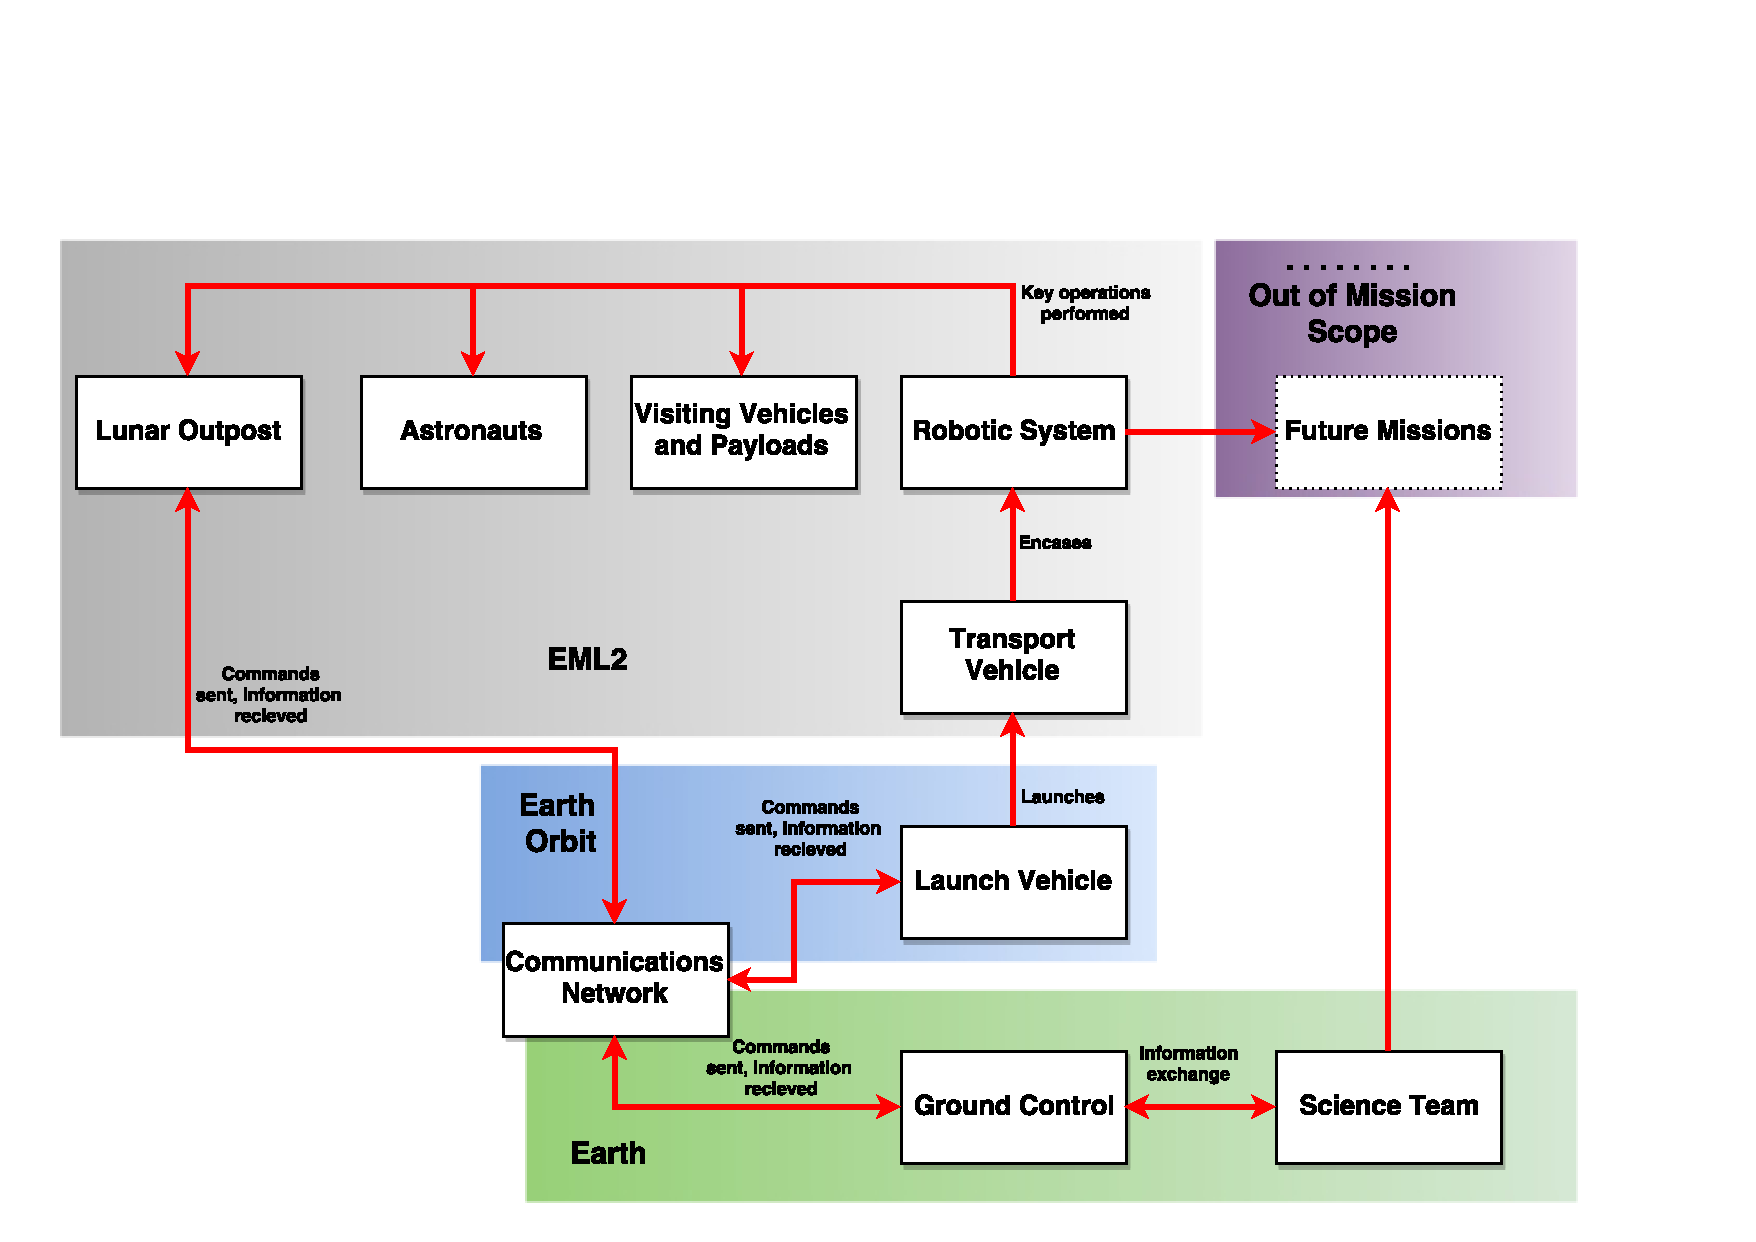
\includegraphics[width=\textwidth, height=\textheight, keepaspectratio]{Figures/MLBD}
\caption{\acrlong{MLBD}}
\label{fig:MLBD}
\end{figure}
			% need description
\newpage
\section{Operational Scenarios}
\label{sect:FFBD}
\vspace{-10pt}
\begin{figure}[H]
\centering
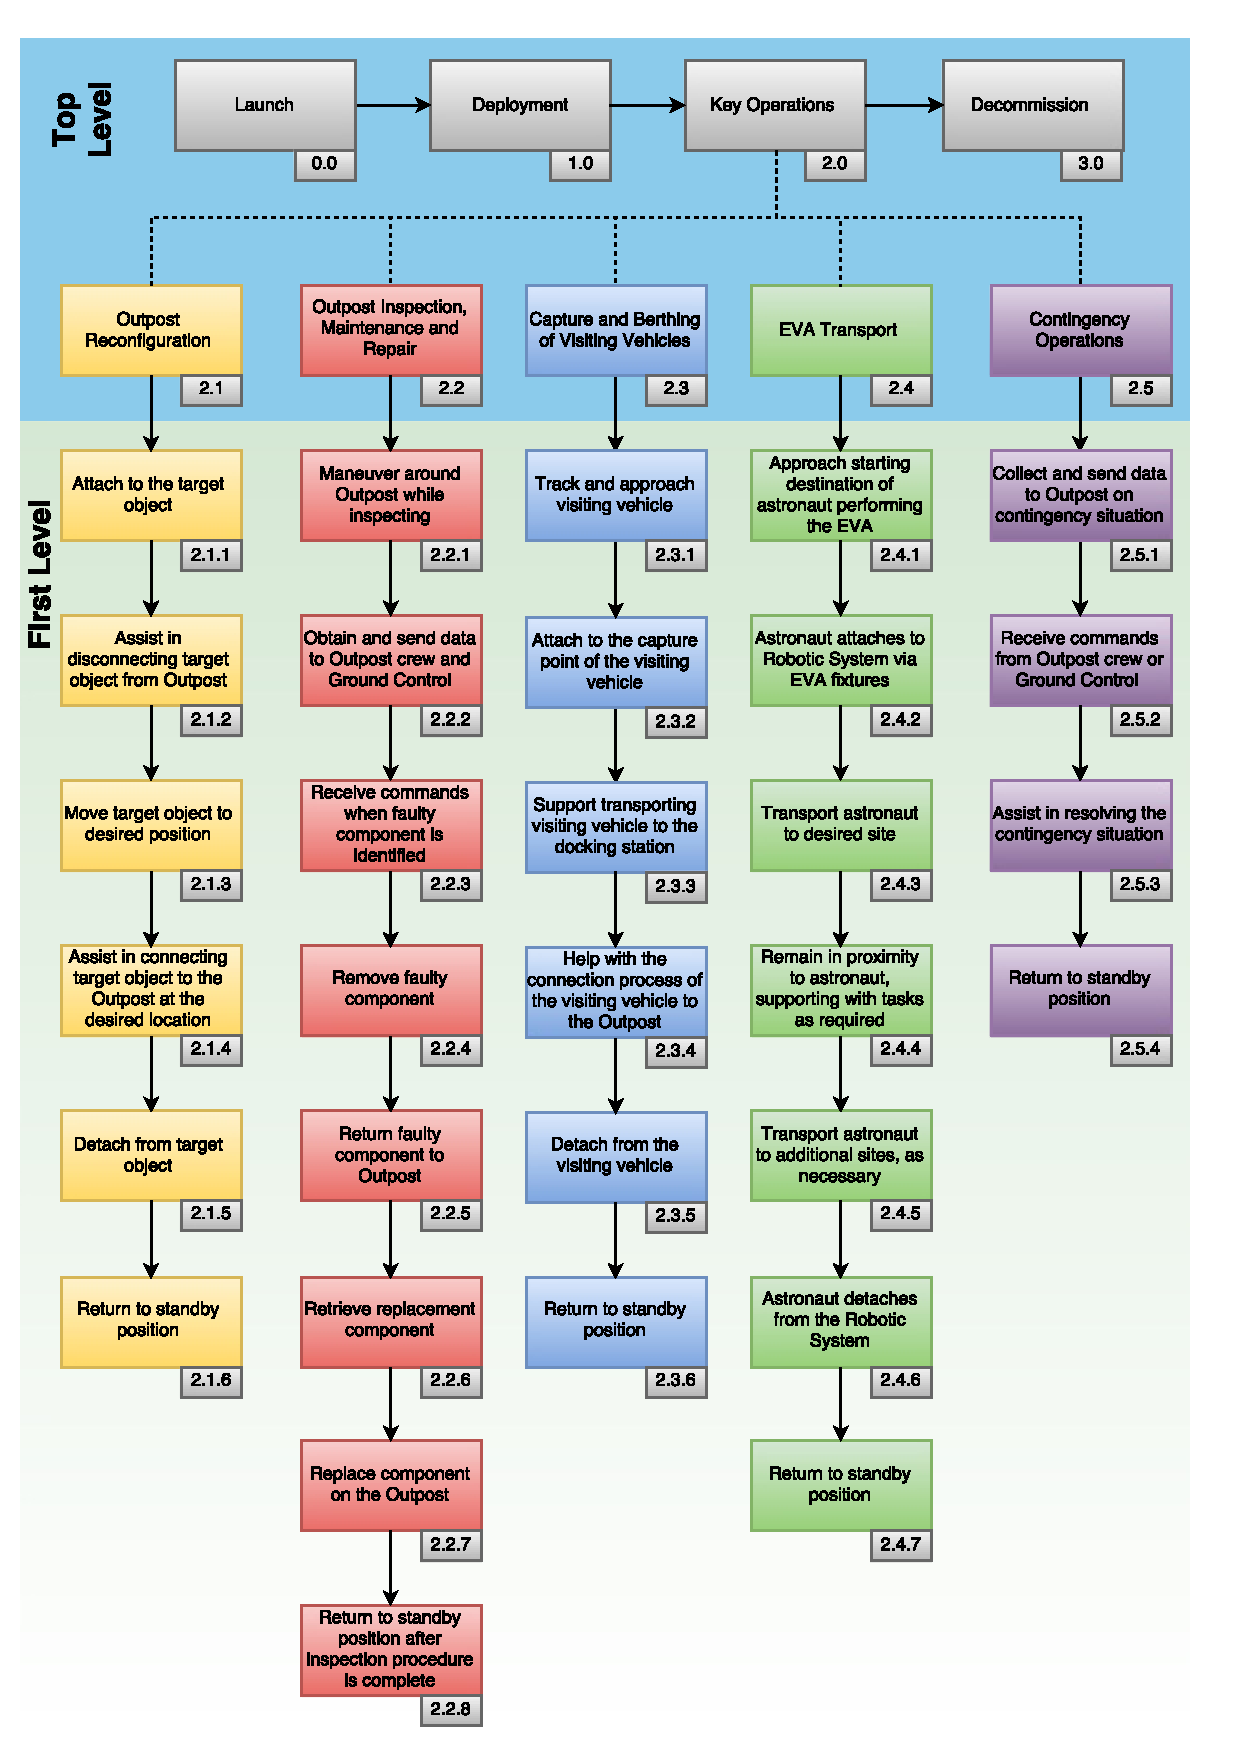
\includegraphics[width=\textwidth, height=0.91\textheight, keepaspectratio]{Figures/FFBD}
\caption{\acrlong{FFBD}}
\label{fig:FFBD}
\end{figure}


\begin{figure}[H]
\centering
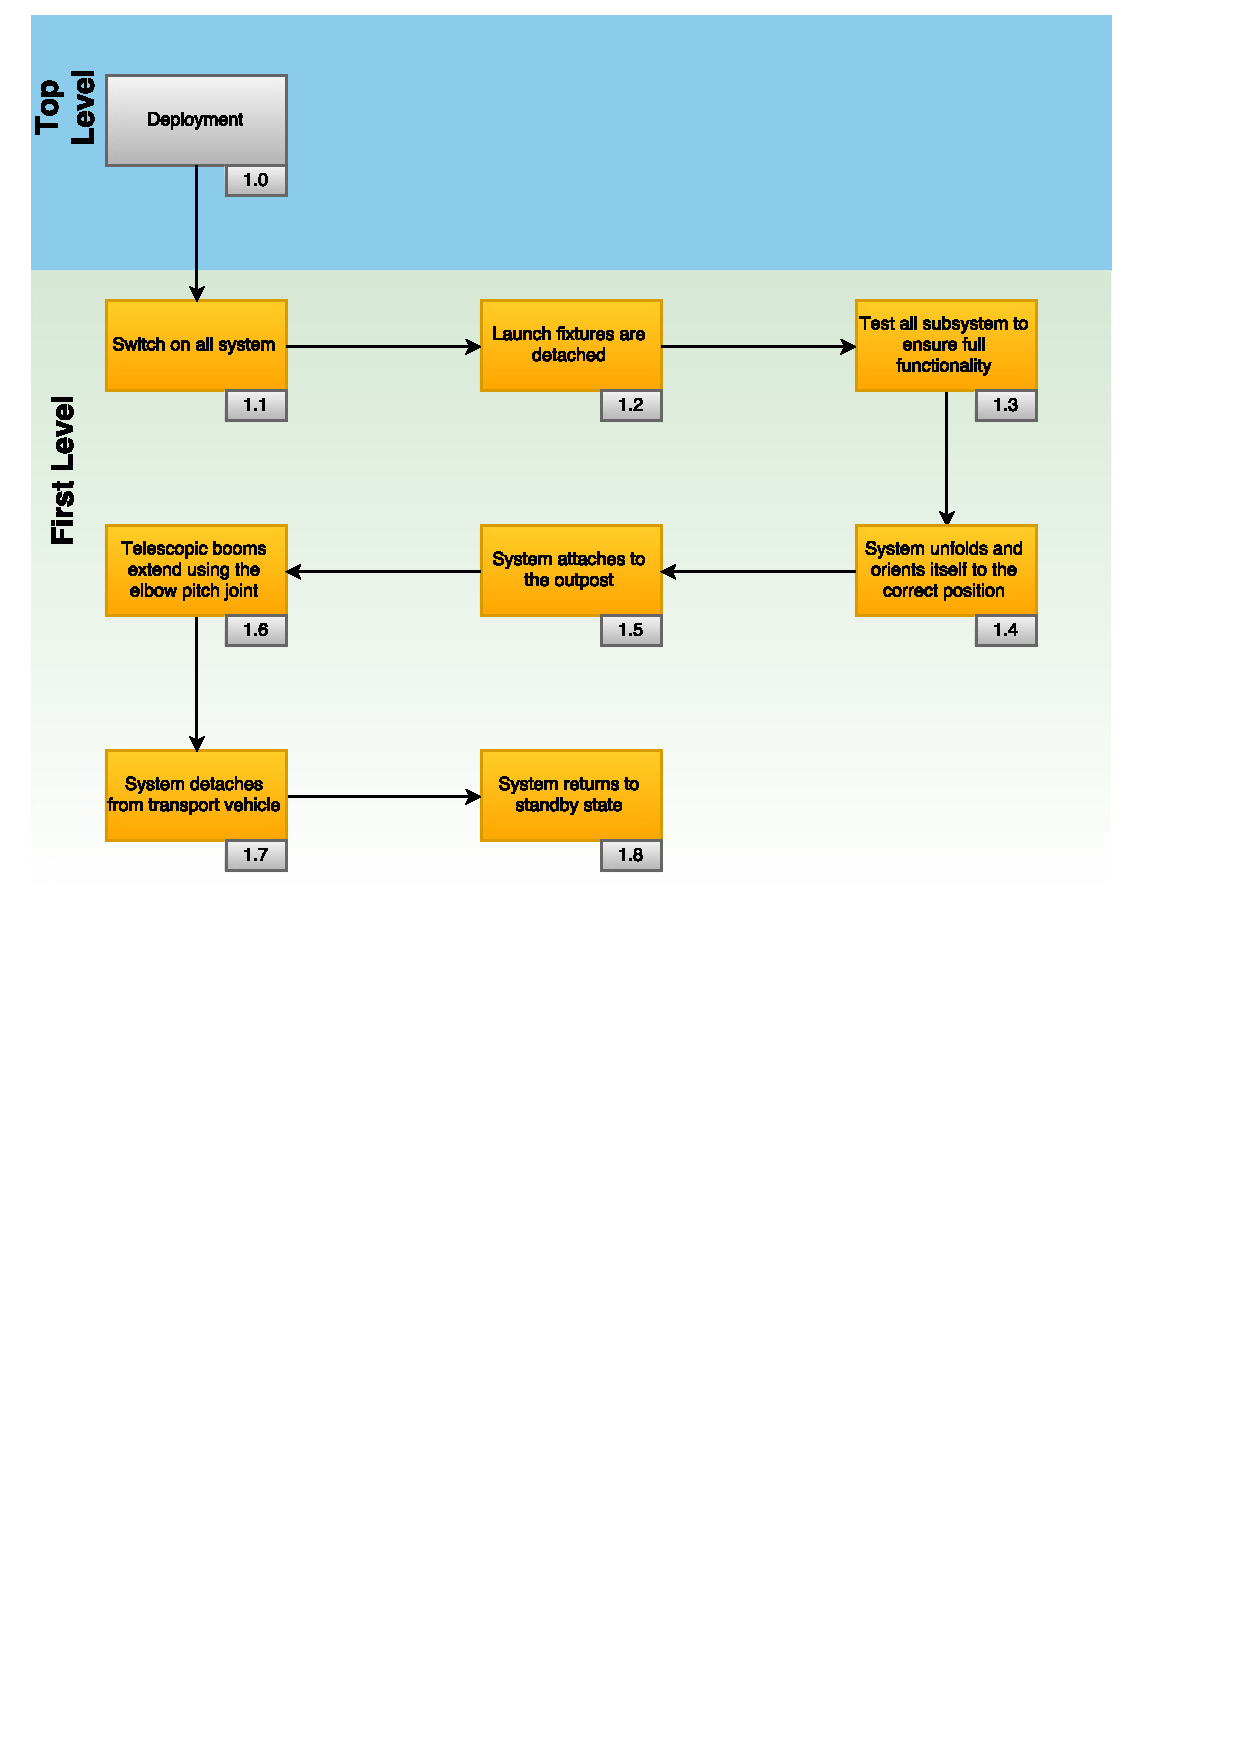
\includegraphics[width=\textwidth, height=0.94\textheight, keepaspectratio]{Figures/FFBD_deploy}
\caption{Deployment \acrshort{FFBD}}
\label{fig:FFBD_deploy}
\end{figure}


\begin{figure}[H]
\centering
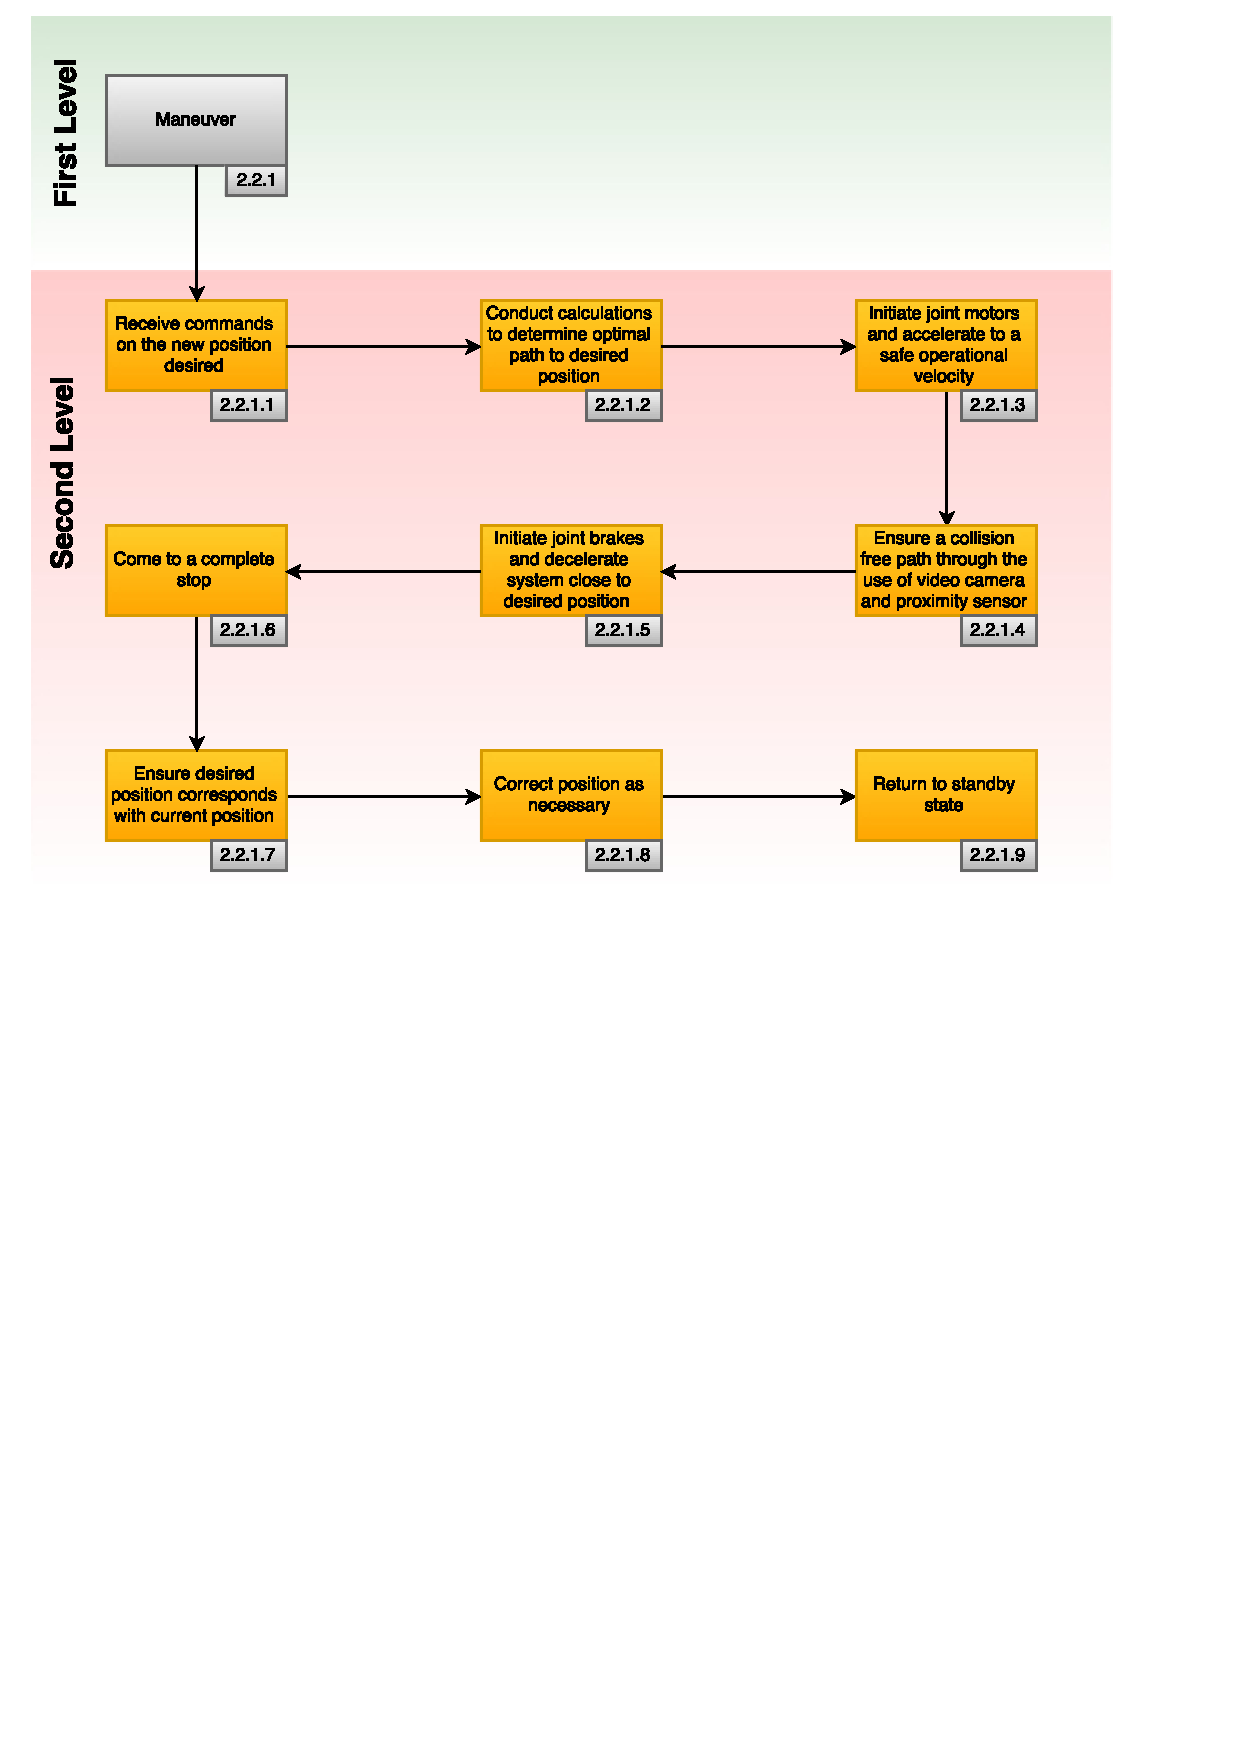
\includegraphics[width=\textwidth, height=0.94\textheight, keepaspectratio]{Figures/FFBD_maneuver}
\caption{Maneuvering \acrshort{FFBD}}
\label{fig:FFBD_manuever}
\end{figure}


\begin{figure}[H]
\centering
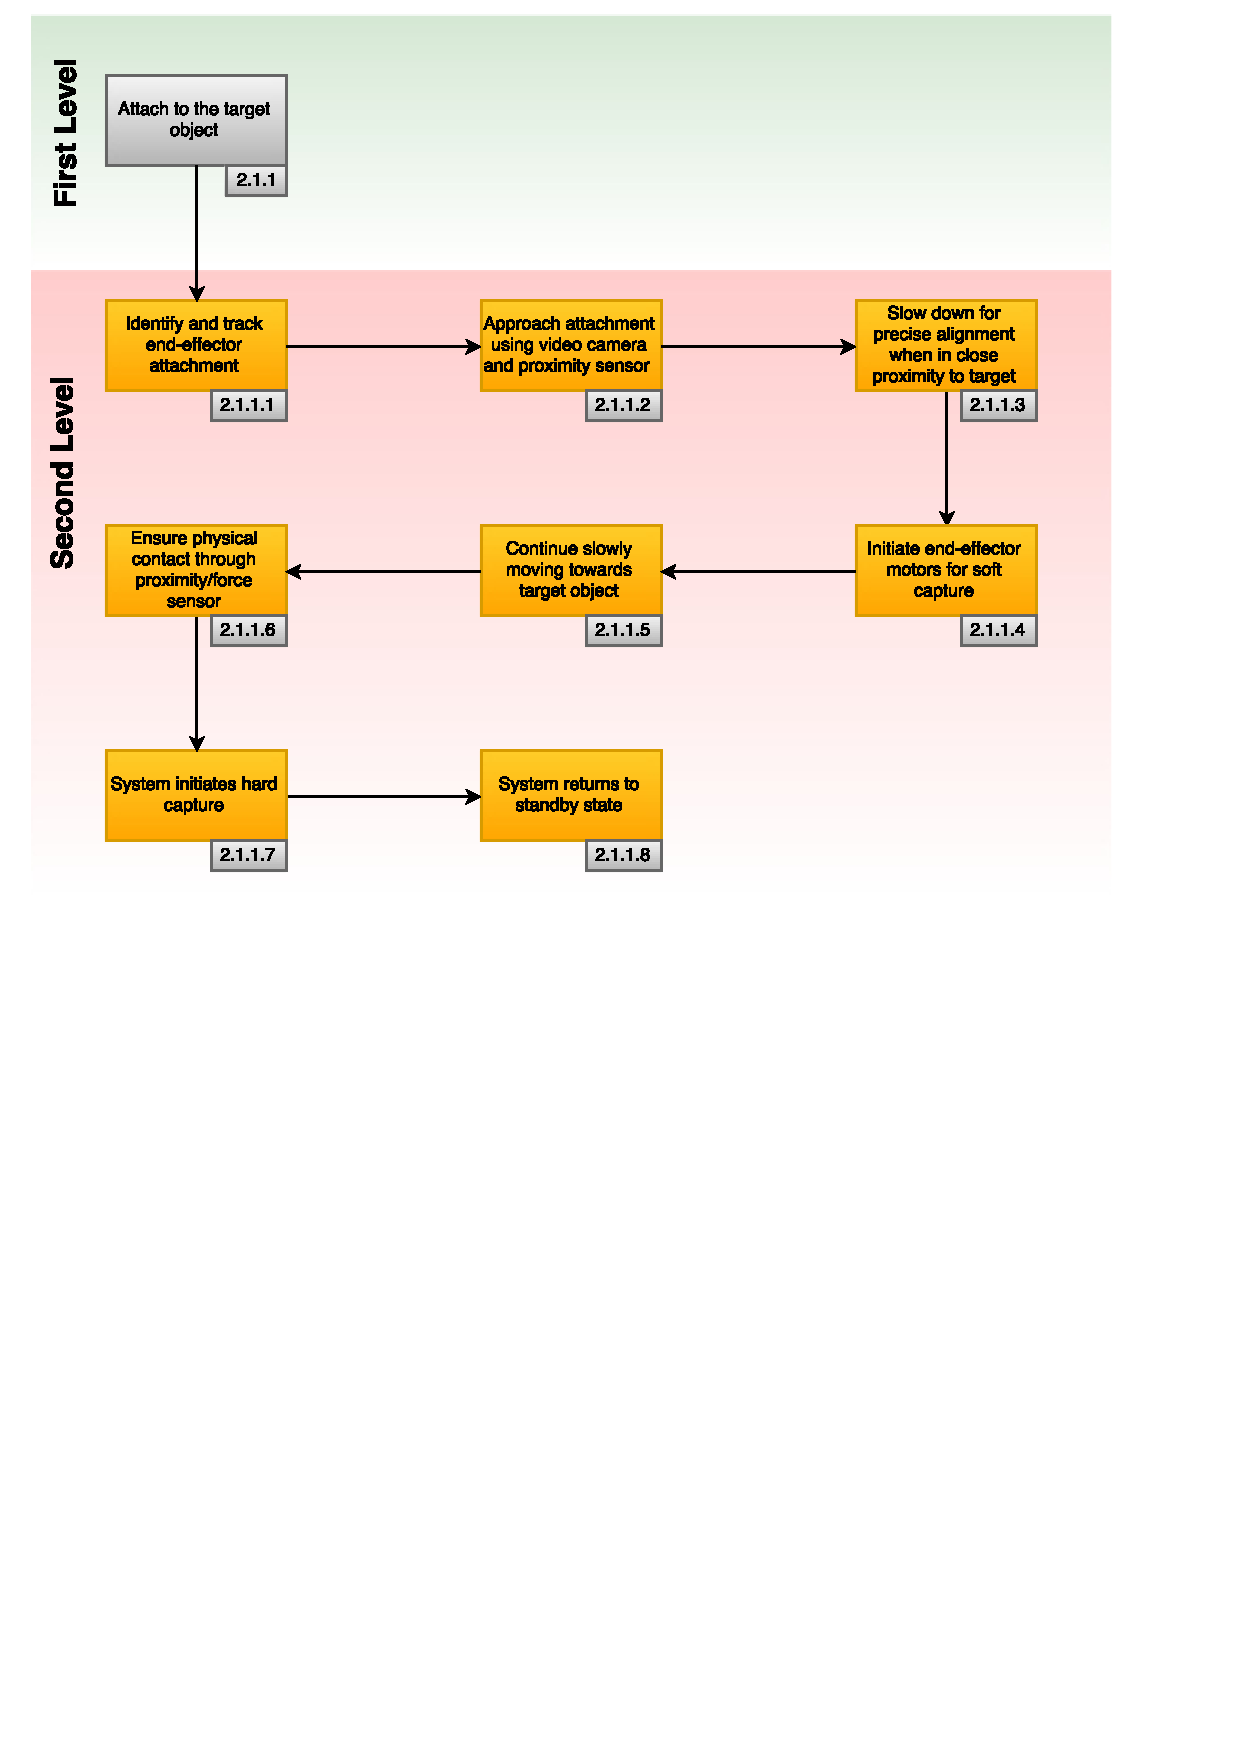
\includegraphics[width=\textwidth, height=0.94\textheight, keepaspectratio]{Figures/FFBD_attach}
\caption{Attaching \acrshort{FFBD}}
\label{fig:FFBD_attach}
\end{figure}


\begin{figure}[H]
\centering
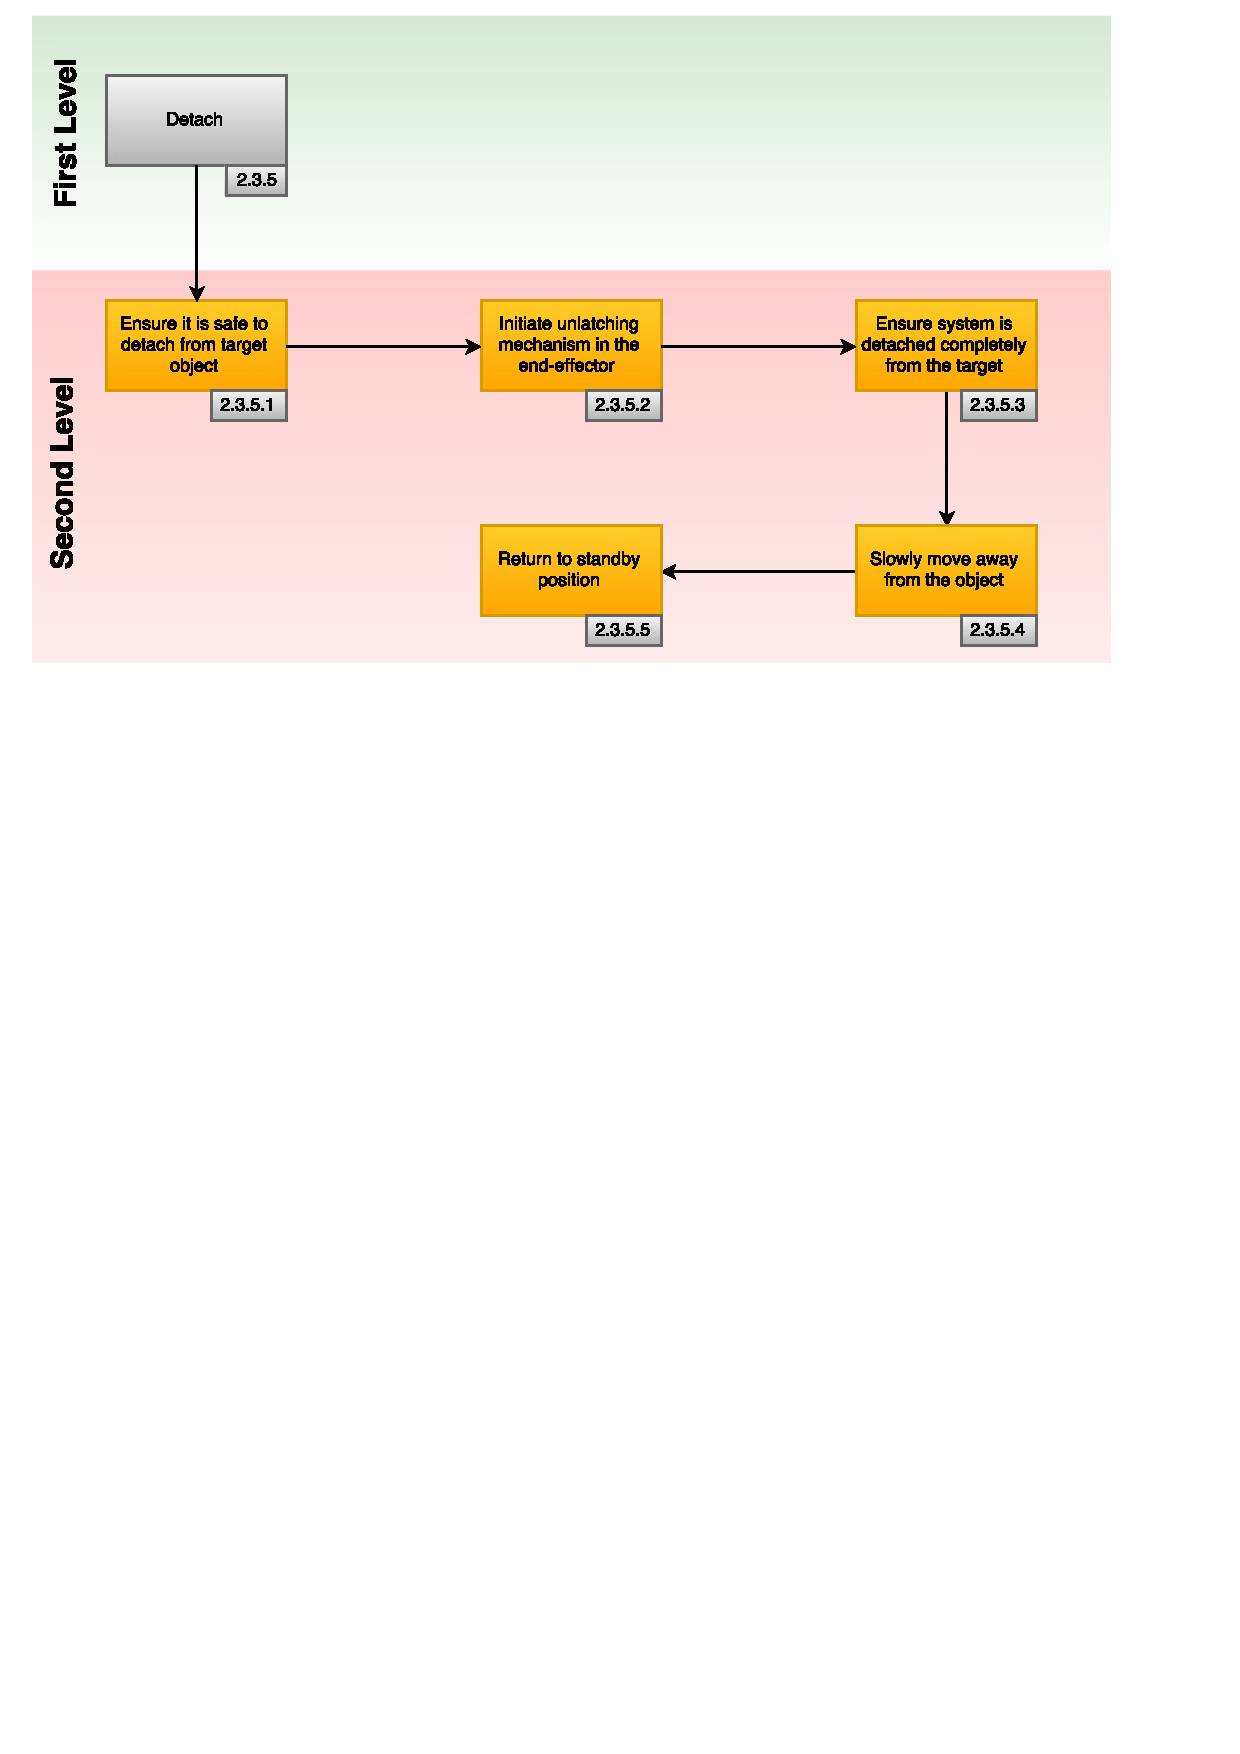
\includegraphics[width=\textwidth, height=0.94\textheight, keepaspectratio]{Figures/FFBD_detach}
\caption{Detaching \acrshort{FFBD}}
\label{fig:FFBD_detach}
\end{figure}			% need description

%--------------System
\begin{landscape}
\section{System Block Diagram}
\label{sect:SBD}
\begin{figure}[H]
\centering
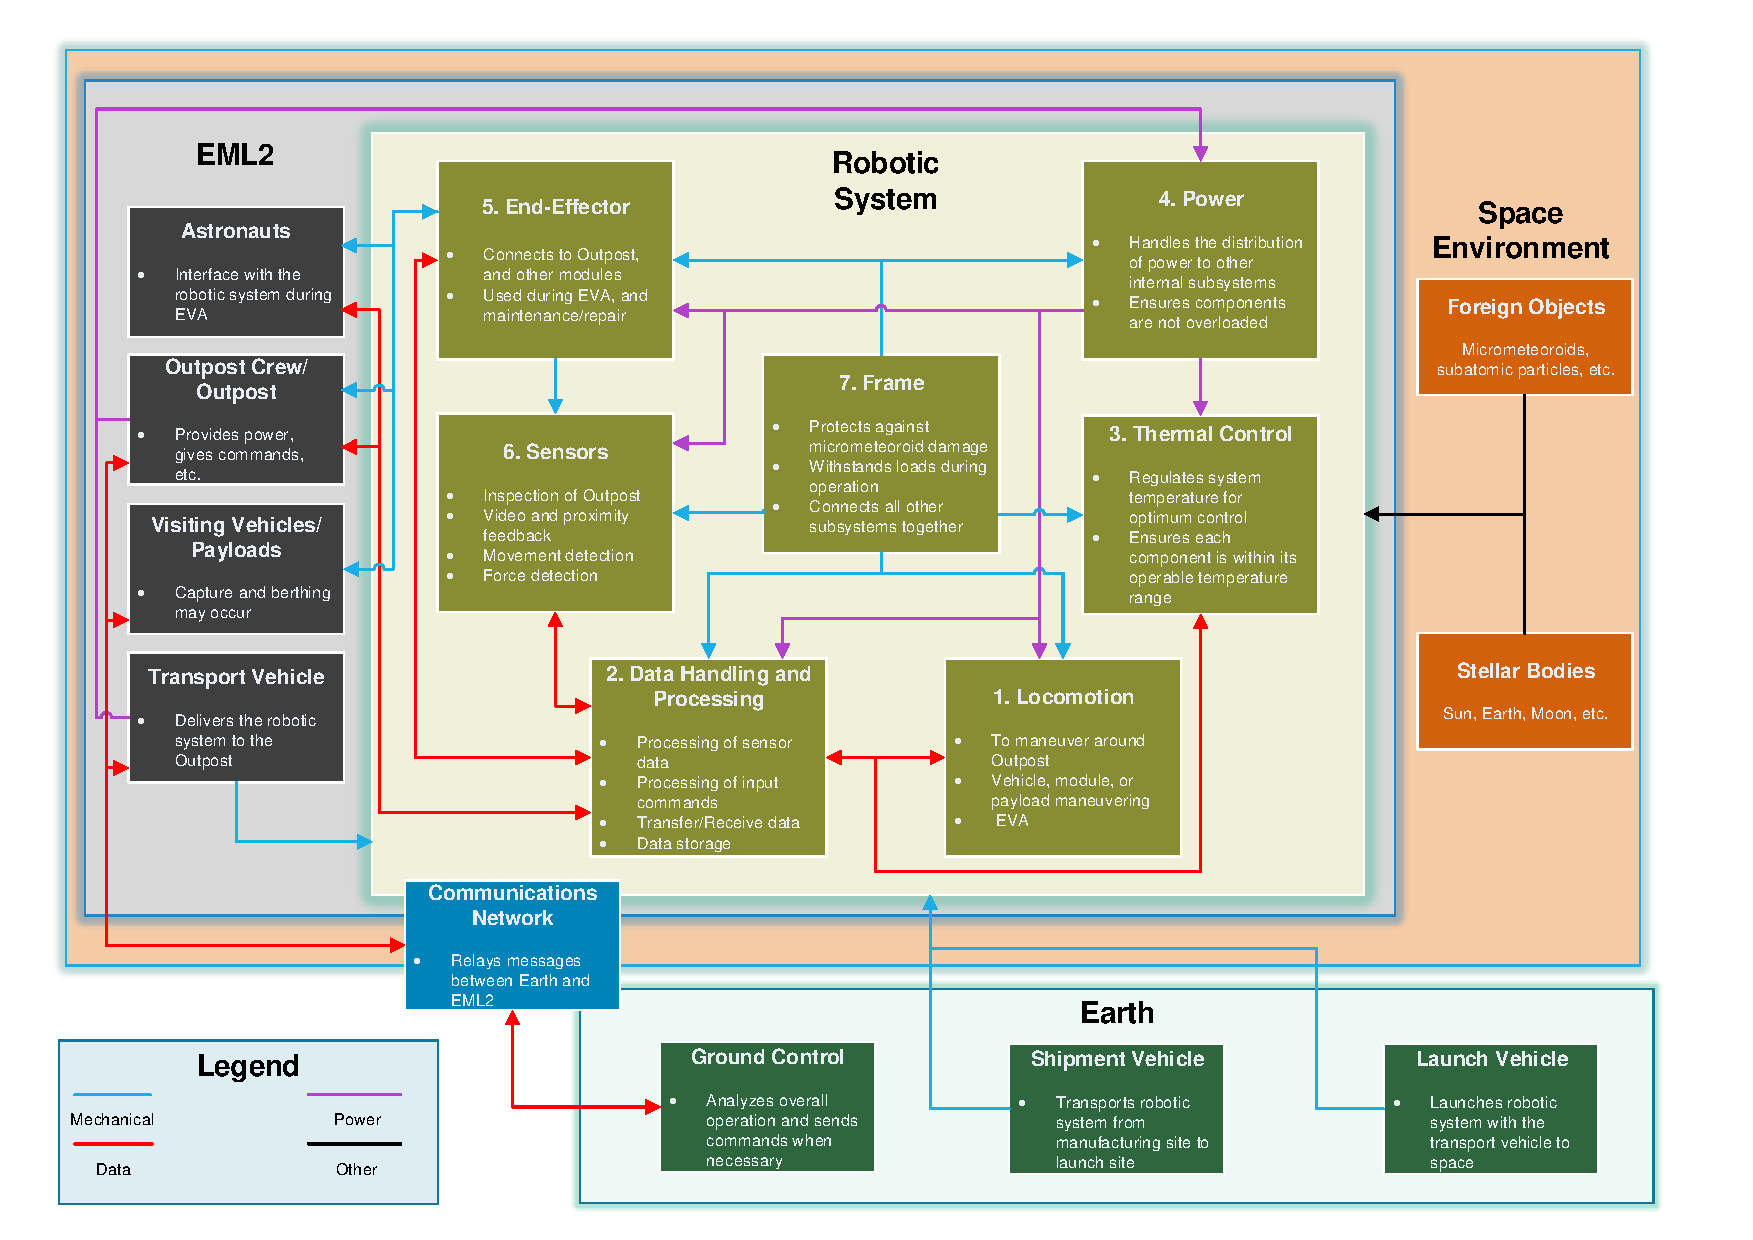
\includegraphics[width=9in, height=5.5in, keepaspectratio]{Figures/SBD}
\caption{\acrlong{SBD}}
\label{fig:SBD}
\end{figure}
				% Done
\newpage
\section{System Hierarchy Diagram}
\label{sect:SHD}
\begin{figure}[H]
\centering
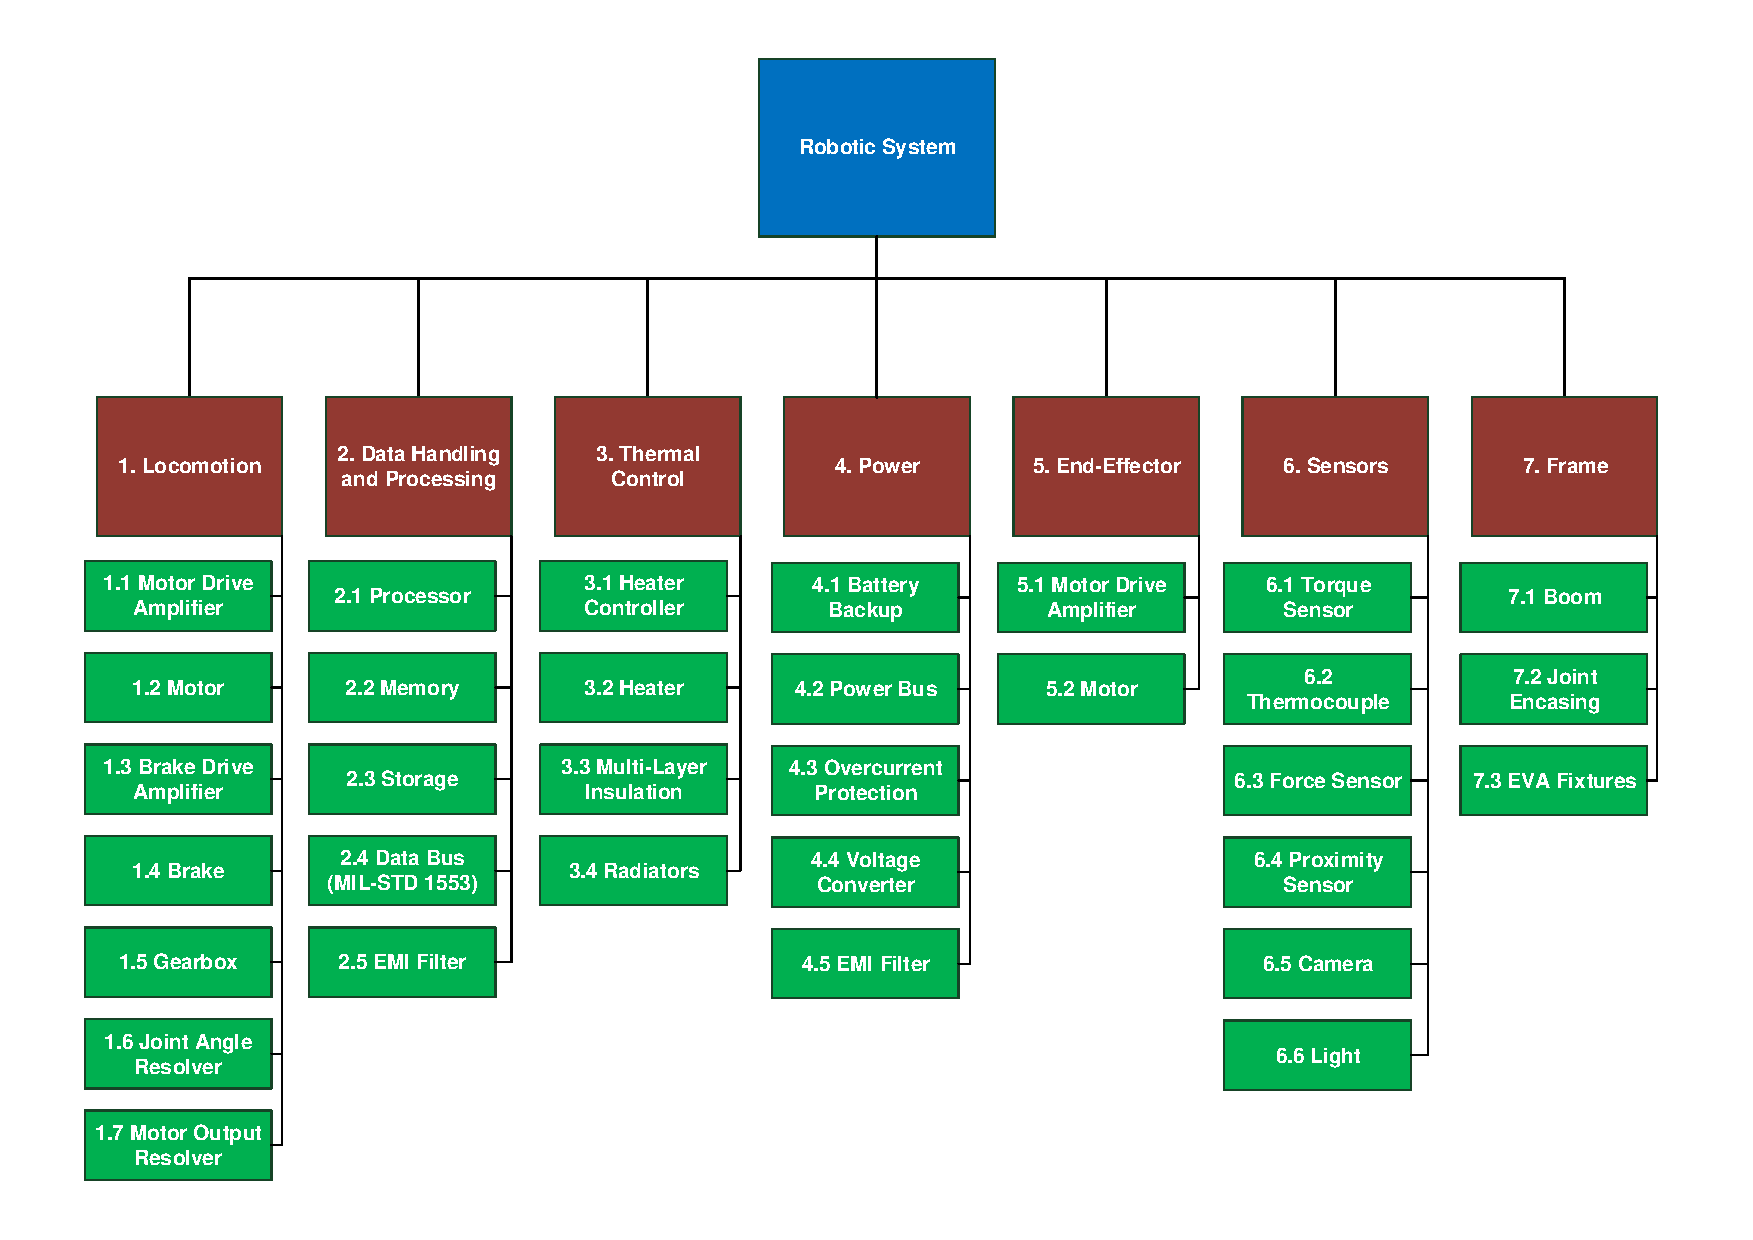
\includegraphics[width=9in, height=5.5in, keepaspectratio]{Figures/SHD}
\caption{\acrlong{SHD}}
\label{fig:SHD}
\end{figure}
				% Done
\end{landscape}

\section{System Requirement}
\captionsetup[table]{list=no}
The following list contains the top-level robotic system requirements. Several of these requirements are drawn from the \gls{RFP} \cite{RFP}. 
%-----------------------------------------------------------------------------------------------------------------------------------------------------------------------------------------------------------------------
\subsection{Functional Requirements}
\begin{longtable}{P{1.5cm}P{14.25cm}}
\vspace{-15pt}
\textbf{S-F-01}	& The system shall be deployable from the transport vehicle. \\
& \textit{Rationale: Derived from \gls{RFP}}	\\
& \textit{Verified by Ground Testing}	\\
\textbf{S-F-02}	& The system shall attach itself to the Outpost. \\
& \textit{Rationale: }	\\
& \textit{Verified by Ground Testing}	\\
\textbf{S-F-03}	& The system shall be able to change the Outpost configuration. \\
& \textit{Rationale: Derived from \gls{RFP}}	\\
& \textit{Verified by Ground Testing}	\\
\textbf{S-F-04}	& The system shall perform inspection of the surface of the Outpost.\\
& \textit{Rationale: }	\\
& \textit{Verified by Ground Testing}	\\
\textbf{S-F-05}	& The system shall perform repairs on the Outpost. \\
& \textit{Rationale: }	\\
& \textit{Verified by Ground Testing}	\\
\textbf{S-F-06}	& The system shall be able to replace faulty components on the Outpost. \\
& \textit{Rationale: }	\\
& \textit{Verified by Ground Testing}	\\
\textbf{S-F-07}	& The system shall send feedback to Outpost crew. \\
& \textit{Rationale: }	\\
& \textit{Verified by Ground Testing}	\\
\textbf{S-F-08}	& The system shall be able to capture visiting vehicles and payloads. \\
& \textit{Rationale: }	\\
& \textit{Verified by Ground Testing}	\\
\textbf{S-F-09}	& The system shall assist in berthing of vehicles and payloads. \\
& \textit{Rationale: }	\\
& \textit{Verified by Ground Testing}	\\
\textbf{S-F-10}	& The system shall operate in \gls{LEO}.\\ 
& \textit{Rationale: }	\\
& \textit{Verified by Ground Testing}	\\
\textbf{S-F-11}	& The system shall operate in Lunar \gls{DRO}. \\
& \textit{Rationale: }	\\
& \textit{Verified by Ground Testing}	\\
\textbf{S-F-12}	& The system shall operate at \gls{EML2}. \\ 
& \textit{Rationale: }	\\
& \textit{Verified by Ground Testing}	\\
\textbf{S-F-13}	& The system shall carry out commands from Ground Control. \\
& \textit{Rationale: }	\\
& \textit{Verified by Ground Testing}	\\
\textbf{S-F-14}	& The system shall carry out commands from the Outpost.\\
& \textit{Rationale: }	\\
& \textit{Verified by Ground Testing}	\\
\textbf{S-F-15}	& The system shall be able to self-manipulate from one spacecraft to another. \\
& \textit{Rationale: }	\\
& \textit{Verified by Ground Testing}	\\
\textbf{S-F-16}	& The system shall be transported from manufacturing facility to launch site.\\
& \textit{Rationale: The robotic system may be manufactured from different site and need to be transported for launch}	\\
& \textit{Verified by Ground Testing}	\\
\end{longtable}
%--------------------------------------------------------------------------------------------------------------------------------------------------------------------------------------------------------------------
\subsection{Performance Requirements}
\vspace{-15pt}
\begin{longtable}{P{1.5cm}P{14.25cm}}
\textbf{S-P-01}	& The system shall manipulate payloads of up to 10000 \gls{kg} \cite{RFP}. \\
& \textit{Rationale: Derived from \gls{RFP}}	\\
& \textit{Verified by Ground Testing}	\\
\textbf{S-P-02}	& The system shall apply holding or reaction forces of 200 \gls{N} in any direction \cite{RFP}. \\
& \textit{Rationale: Derived from \gls{RFP}}	\\
& \textit{Verified by Ground Testing}	\\
\textbf{S-P-03}	& The system shall withstand LOS for up to 30 \gls{min}.\\ & \textit{Rationale: Derived from \gls{RFP}}	\\
& \textit{Verified by Ground Testing}	\\
\textbf{S-P-04}	& The system shall operate for 10 years  \cite{RFP}. \\
& \textit{Rationale:Derived from \gls{RFP}}	\\
& \textit{Verified by Ground Testing and Analysis}	\\
\textbf{S-P-05}	& The working envelope (work area) of the system shall cover TBD \% of the surface area of the Outpost. \\
& \textit{Rationale: Required for maintenance and inspection operation}	\\
& \textit{Verified by Ground Testing and Analysis}	\\
\end{longtable}
%-----------------------------------------------------------------------------------------------------------------------------------------------------------------------------------------------------------------------
\subsection{Constraint Requirements}
\vspace{-15pt}
\begin{longtable}{P{1.5cm}P{14.25cm}}
\textbf{S-C-01}	& The system shall have a mass of less than 450 \gls{kg} \cite{RFP}. \\
& \textit{Rationale: Derived from \gls{RFP} }	\\
& \textit{Verified by analyzing mass of the system before launch}	\\
\textbf{S-C-02}	& The system shall be able to fit into transport vehicle \cite{RFP}. \\
& \textit{Rationale: System needs to be transported inside a vehicle for transportation}	\\
& \textit{Verified by measuring dimensions of the system}\\
\textbf{S-C-03}	& The system shall have an average power usage of 450 \gls{W} \cite{RFP}.\\
& \textit{Rationale: Derived from \gls{RFP}}	\\
& \textit{Verified by Ground Testing}						\\
\textbf{S-C-04}	& The system shall have a peak power usage of 600 \gls{W} at 28 \gls{V} \cite{RFP}. \\
& \textit{Rationale: Derived from \gls{RFP}}	\\
& \textit{Verified by Ground Testing}						\\
\textbf{S-C-06}	& The system shall have single fault tolerance under all operations.\\
& \textit{Rationale: Required for System operation}	\\
& \textit{Verified by Ground Testing \& Simulation}	\\
\end{longtable}
%-----------------------------------------------------------------------------------------------------------------------------------------------------------------------------------------------------------------------
\subsection{Environmental Requirements}
\vspace{-15pt}
\begin{longtable}{P{1.5cm}P{14.25cm}}
\textbf{S-E-01}	& The system shall operate in a vacuum environment.\\
& \textit{Rationale: Operational environment is vacuum}	\\
& \textit{Verified by Ground Testing}\\
\textbf{S-E-02}	& The system shall operate within temperature ranges of -90\gls{degC} to 200\gls{degC} \cite{NASAsysreq_Kumar}.\\
& \textit{Rationale: Derived from temperature range in the operational environment}	\\
& \textit{Verified by Ground Testing and Simulation}\\
\textbf{S-E-03}	& The system shall withstand vibrations sustained during transport to launch site.\\
& \textit{Rationale: Vibration may damage parts in the system}	\\
& \textit{Verified by Ground Testing}\\
\textbf{S-E-04}	& The system shall withstand vibrations sustained during launch.\\
& \textit{Rationale: Vibration may damage parts in the system}	\\
& \textit{Verified by Ground Testing}\\
\textbf{S-E-05}	& The system shall withstand electromagnetic radiation of 1300 \gls{W/m2}(\gls{TBC})  \cite{FAA_radiation}.\\
& \textit{Rationale: Radiation affects the surface of the system, electronics, and communication}	\\
& \textit{Verified by Ground Testing}\\
\textbf{S-E-06}	& The system shall withstand solar flares.\\
& \textit{Rationale: Solar flares affect the surface of the system, electronics, and communication}	\\
& \textit{Verified by Ground Testing}\\
\textbf{S-E-07}	& The system shall withstand cosmic rays.\\  
& \textit{Rationale: Cosmic rays affect the surface of the system, electronics, and communication}	\\
& \textit{Verified by Ground Testing}\\
\textbf{S-E-08}	& The system shall withstand strikes by foreign objects with \gls{TBD} momentum. \\
& \textit{Rationale: Foreign objects may damage the surface of the system and the sensors}	\\
& \textit{Verified by Ground Testing}\\
\end{longtable}
%---------------------------------------------------------------------------------------------------------
\subsection{Drivers}
The following five requirements are identified as the key design drivers, which will heavily influence the outcome of system design.

\textbf{S-P-01: The system shall manipulate payloads of up to 10000 \gls{kg} \cite {RFP}.}

The requirement that the payloads shall be up to 10000 \gls{kg} affects the design of all subsystems. This driver influences the materials chosen for the frame, and end-effector. It also affects the types of sensors used on the robotic system and method of locomotion. In addition, design decisions regarding how the system is able to capture/berthing of visiting vehicles and complete Outpost reconfiguration will be influenced by this driver.

\textbf{S-P-02: The system shall apply holding or reaction forces of 200 \gls{N} in any direction \cite{RFP}.}

The requirement that the system shall apply holding or reaction forces of \SI{200}{\N} in any direction is closely related to the EVA and Outpost Repair operations. The design of the end-effector and types of sensors used on the robotic system will be affected by this driver. It also influence the locomotion subsystem as the design of mobility method is affected. And the design of the frame subsystem is naturally affected by this requirement as all these other subsystems changes.

\textbf{S-P-05: The working envelope (work area) of the system shall cover \gls{TBD} \% of the surface area of the Outpost.}

The requirement that the working envelope (work area) of the system shall cover TBD \% of the surface area of the Outpost influences the locomotion and end-effector design, as well as the positioning of sensors to ensure that the sensor subsystem is able to analyze the Outpost in detail. In addition, design decisions regarding how the system is able to reach to the ends of the working envelope would also have to be decided. Naturally, the frame subsystem is affected as the design of the robotic system changes.

\textbf{S-C-01: The system shall have a mass of less than 450 \gls{kg} \cite{RFP}.}

The constraint on mass affects the design of all subsystems. This driver influences the materials chosen for the frame, and end-effector subsystem. Additionally, the method of power supply, the types and amounts of sensors used on the robotic system is affected, as well as the hardware of the data handling, and thermal control subsystem. All these design decisions need to be made to fulfill the overall mass requirement. Moreover, the weight of the whole system will also have an influence on the method of shipment.

\textbf{S-C-04: The system shall have an average power usage of 450 \gls{W} \cite{RFP}.}

The power constraint influences all electrical components of the robotic system. It affects the types of sensors selected, the method of power supply and power backup, as well as the hardware choice of the data handling and processing, and thermal control subsystems. In order to complete all the operations within the power constraint, the mobility method of locomotion subsystem and electrical hardware of the data handling subsystem will also be influenced.			% Done
\captionsetup[table]{list=yes}
\setcounter{table}{\ref{risktable}}

\section{System Level Trade Studies}
\subsection{Mechanical Tradeoffs}
%----------------------------Autonomy---------------------------
\subsubsection{Level of Autonomy}
The level of autonomy will determine how the operations should be planed and carried out, and will largely influence the design of data handling and control systems. Therefore, it should be discussed here as one of the major trade-offs. Three levels of autonomy are considered and compared, which are listed below and compared in \Cref{tab:auto}. A limited-autonomous system requires Requires manual operations by the Outpost crew to complete all tasks, a semi-autonomous system shall be able to conduct basic tasks automatically, like change positions, but will require manual control by Outpost crew to complete more complex tasks while a fully-autonomous system shall be able to complete both all tasks without human intervention. 

\begin{longtable}{|P{2.5cm}|P{4.1cm}|P{4.1cm}|P{4.0cm}|}
\caption{Trade Study for Level of Autonomy}\label{tab:auto}\\
\hline
&	\textbf{Limited Autonomous}	&	\textbf{Semi Autonomous}	&	\textbf{Fully Autonomous}	\\\hhline{|=|=|=|=|}
\endfirsthead
\hline
&	\textbf{Limited Autonomous}	&	\textbf{Semi Autonomous}	&	\textbf{Fully Autonomous}	\\\hhline{|=|=|=|=|}
\endhead
\textbf{System Complexity}	&	\textcolor{OliveGreen}{Easy to develop\newline Rich technological heritage}	&	\textcolor{OliveGreen}{Existing similar systems}\newline \textcolor{red}{Need software development for the specific operations}	&	\textcolor{red}{Technology is hard to achieve\newline Full software development needed}	\\\hline
\textbf{System Reliability}	&	\textcolor{OliveGreen}{Operation is fully monitored}\newline \textcolor{red}{Human errors may occur}	&	\textcolor{red}{Simple tasks may be affected by software and component malfunctions}\newline \textcolor{orange}{Complex tasks may be affected by human errors}	&	\textcolor{OliveGreen}{Human error is avoided.}\newline \textcolor{red}{Operation could be under software and component malfunctions \cite{malfunction}}	\\\hline
\textbf{Operation Duration}	&	\textcolor{red}{Requires control from the Outpost crew or Astronauts\newline Crew time usage on redundant tasks}	&	\textcolor{OliveGreen}{Short for simple tasks}\newline\textcolor{red}{Longer duration for more complex tasks}	&	\textcolor{OliveGreen}{ No human input required\newline Can operate continuously}	\\\hline
\textbf{Operation Accuracy \& Deviation from plans}	&	\textcolor{OliveGreen}{Deviation from plans is limited by human control}\newline\textcolor{red}{May be affected by human errors}	&	\textcolor{OliveGreen}{Simple Task: not limited by computational resources.
\newline Complex Task: Human errors and robotic malfunctions are limited}	&	\textcolor{red}{Limited by computational and power resources}	\\\hline
\end{longtable}

While a fully autonomous system would be ideal for space exploration because it would have high capabilities and efficiency, there are still technical, computational, safety and managerial challenges to overcome before achieving full autonomy. Therefore, taking current technology availability into consideration, a semi-autonomous system has been selected for this robotic system. This will allow the system to perform with relatively lower risk and higher efficiency.

%----------------------------Thermal---------------------------
\subsubsection{Thermal Control System}
Thermal regulation systems are required in the system to ensure that temperatures of the system's parts are within the operating ranges. There are two main types of such systems, \gls{ATCS} and \gls{PTCS}. 

\gls{ATCS} makes use of various heating and cooling tools, such as electric heaters, fluid loops and thermoelectric coolers to control the temperature within the system while \gls{PTCS} makes use of insulation to reduce heat transfer and surface coatings which modify the thermal or optical properties of the surface. These two systems are compared in \Cref{table:thermal}.
\begin{table}[H]
\caption{Trade Study for Type of Thermal Control System}
\begin{tabular}{|P{2.5cm}|P{6.35cm}|P{6.35cm}|}
\hline
	&	\textbf{\gls{ATCS} \cite{thermal_sys}}	&	\textbf{\gls{PTCS} \cite{thermal_sys}}	\\\hhline{|=|=|=|}
\textbf{System Complexity}	&	\textcolor{red}{Complex control system needed to respond rapidly to temperature fluctuations}	&	\textcolor{OliveGreen}{Only mechanical parts are added}	\\\hline
\textbf{System Reliability}	&	\textcolor{OliveGreen}{Outpost crew can manually control the temperature in case of breakdown in control system}\newline\textcolor{orange}{In case of breakdown of the heating and/or cooling elements, only solution is to repair them}	&	\textcolor{red}{Damage will result in loss of ability to maintain other subsystems at their operational temperature ranges}	\\\hline
\textbf{System Efficiency}	&	\textcolor{OliveGreen}{System can be on Standby mode when temperatures are within operating ranges\newline Only needs to be switched on when temperature is near the limits of operation; Saves power and does its job}	&	\textcolor{OliveGreen}{System can reduce heat transfer without using any power; Very efficient when there is alternating high and low temperatures}\newline\textcolor{orange}{System is unable to regulate temperatures when there is prolonged periods of extreme temperatures}	\\\hline
\end{tabular}
\label{table:thermal}
\end{table}
According to some further research, it is actually possible to combine these two choices to a semi-active thermal control system \cite{comb_thermal}, which is selected to be used on our robotic system. The main system will be the passive system to slow down the rate of heat transfer between internal components and the exterior environment. The active system will activate when there is excessive heat transfer that the passive system is unable to manage, or when there is damage to the passive system. This allows us to achieve the advantages of power saving and single-fault tolerance in the thermal control system, but we would have to accept the consequence of increasing the mass of the system and designing a more complex control architecture for the active system.

\subsection{Electrical Tradeoffs}
%----------------------------Power---------------------------
\subsubsection{Power Generation and Storage System}
Power supply system is required in the system to distributing power to other subsystems and ensuring they function properly. A system level tradeoff on the method of power supply system is discussed in this section. Two options are considered, one is to have an independent power generation system, such as solar panels; the other is to have the robotic system fully powered by the Outpost. \Cref{tab:power} below provides a detailed comparison between these two options.

\begin{table}[H]
\caption{Trade Study for Power Generation and Storage System}
\begin{tabular}{|P{3cm}|P{6.1cm}|P{6.1cm}|}
\hline
	&	\textbf{Independent Power System}	&	\textbf{Powered by Outpost}	\\\hhline{|=|=|=|}
\textbf{System Complexity}	&	\textcolor{red}{Significantly increase the system complexity}	&	\textcolor{OliveGreen}{Simple system}	\\\hline
\textbf{Mass Required}	&	\textcolor{red}{Significantly increase the mass \newline Common option like solar panels typically cost about 0.02 \gls{kg} per \gls{W} \cite{solar_panel}}	&	\textcolor{OliveGreen}{Lower mass, mainly cost by connection cables}	\\\hline
\textbf{System Independence}	&	\textcolor{OliveGreen}{Can operate without connection to the Outpost }	&	\textcolor{red}{Unable to operate  on loss of connection to Outpost \newline If mobile, has to return to the Outpost periodically to recharge}	\\\hline
\end{tabular}
\label{tab:power}
\end{table}

Taking into account the mass constraint, which is one of the main drivers of this project, it is decided that the system will not have its own power generation unit and would instead be powered entirely by the Outpost.\\
However, the system will have a power storage system onboard, which will be charged while the system is connected to the Outpost and can be used in emergency situations when there is a loss in connection between the Outpost and the robotic system. Further details of the power storage system is discussed in \Cref{sect:elec_to}.


\subsection{Control/Software Tradeoffs}
%----------------------------Communication---------------------------
\subsubsection{Communication Link}
For the system level tradeoff on communication link, two options are considered. The first one is to direct communication link with only the Outpost, and the second option is to have direct communication link with both Ground Control and the Outpost. They are compared in \Cref{tab:communication} below.

\begin{table}[H]
\caption{Trade Study for Communication Link}
\begin{tabular}{|P{2.6cm}|P{6.3cm}|P{6.3cm}|}
\hline
	&	\textbf{Direct communication link with only the Outpost}	&	\textbf{Direct communication link with Ground Control \& the Outpost}	\\\hhline{|=|=|=|}
\textbf{System Complexity}	&	\textcolor{OliveGreen}{Relatively Simple control system}	&	\textcolor{red}{Complex control system}	\\\hline
\textbf{Design Constraints}	&	\textcolor{OliveGreen}{Will not increase mass, and low in power comsumption}	&	\textcolor{red}{Will significantly increase the mass and power consumption}	\\\hline
\textbf{Operation Risk}	&	\textcolor{red}{Will completely lose  communication if disconnected from the Outpost}	&	\textcolor{OliveGreen}{Backup communication with Ground System is available if disconnected from the Outpost}	\\\hline
\end{tabular}
\label{tab:communication}
\end{table}

According to \Cref{tab:communication}, having direct communication link with only the Outpost has a significant advantage in mass/power consumption, which matches the main drivers defined. Also, previous space robotic arms like Canadarm2 and \gls{ERA} are both typically operated from the \gls{ISS} \cite{ca_era_communication}. In addition, direct communication with the Ground Control might be impractical because of the time lag in command signals \cite{roboserve}. Hence, it has been decided that our system will contain a communications subsystem to communicate only with the Outpost.
		% Done
%--------------Subsystem Requirement-------------------------------
\newpage
\section{Subsystem Requirements}	% Done
\label{sect:Subsystem Requirements}
\captionsetup[table]{list=no}
\subsection{Subsystem LM: Locomotion}
\label{sect:LM_req}
%---------------------------------------------------------------------------------------------------------
% Mechanical - Rewrite some?
%---------------------------------------------------------------------------------------------------------
\subsubsection*{Functional Requirements}
\captionsetup[table]{list=no}
\vspace{-15pt}
\begin{longtable}{P{2cm}P{13.75cm}}
\textbf{LM-F-01}	&
The locomotion subsystem shall be able to move the robotic system.
\textit{(Derived from S-F-02, S-F-03, S-F-04)}\\
& \textit{Rationale: Required for operation}	\\
& \textit{Verified by ground testing}	\\
\textbf{LM-F-02}	&
The locomotion subsystem shall be functional in a vacuum environment.
\textit{(Derived from S-E-01)}	\\
& \textit{Rationale: Required for operation}	\\
& \textit{Verified by ground testing}	\\
% Electrical ---------------------------------------------------------------------------------------------
\textbf{LM-F-03}	& The locomotion subsystem shall accept electrical power from the power supply subsystem.
\textit{(Derived from S-C-03, S-C-04)}	\\
& \textit{Rationale: subsystem needs power to operate}	\\
& \textit{Verified by ground testing}	\\
\textbf{LM-F-04}	& The locomotion subsystem shall receive commands from the data handling subsystem.
\textit{(Derived from S-F-13, S-F-14)}\\ 
& \textit{Rationale: required for control from ground control or Outpost}\\
& \textit{Verified by ground testing}	\\

\textbf{LM-F-05}	&
The locomotion subsystem shall manipulate the velocities of joints with rates specified by received commands.
\textit{(Derived from S-F-02, S-F-04, S-F-05, LM-F-01)}\\
 &	\textit{Rationale: required for operation} \\
 &	\textit{Verified by ground testing}	\\
 
\textbf{LM-F-06}	&
The locomotion subsystem shall transmit data related to position and angle of the joints to the data handling subsystem. \textit{(Derived from S-F-07)} \\
 &	\textit{Rationale: data handling subsystem will process the data and send necessary information to the Outpost} \\
 &	\textit{Verified by ground testing}
\end{longtable}
%Mechanical------------------------------------------------------------------------------------------------
\vspace{-15pt}
\subsubsection*{Performance Requirements}
\vspace{-15pt}
\begin{longtable}{P{2cm}P{13.75cm}}
\textbf{LM-P-01}	&
The locomotion subsystem shall have at least 6 \gls{DOF}.
\textit{(Derived from S-F-02)}	\\
& \textit{Rationale: Derived from mechanical trade study}	\\
& \textit{(Verified by analysis of the subsystem design)}	\\

\textbf{LM-P-02}	&
The work envelope of the locomotion subsystem shall cover \gls{TBD} \% of the lunar Outpost.
\textit{(Derived from S-P-05)} \\
&	\textit{Rationale: Required for Operation} \\
& \textit{(Verified by ground testing)}	\\

\textbf{LM-P-03}	&
The locomotion subsystem shall move at \gls{TBD} \gls{m/s}.
\textit{(Derived from LM-F-05)}	\\
& \textit{Rationale: Required for Operation} \\
& \textit{(Verified by ground testing)}	\\

\textbf{LM-P-04}	&
The locomotion subsystem shall maintain mechanical integrity between -120\gls{degC} to 180\gls{degC} (\gls{TBC}) \cite{ERAjoint}.
\textit{(Derived from S-E-02)}	\\
& \textit{Rationale: To ensure system operation in the operation temperature range} \\
& \textit{(Verified by ground testing under temperature range)}	\\

\textbf{LM-P-05}	&
The locomotion subsystem shall have a mass less than 141.75 \gls{kg}.
\textit{(Derived from S-C-01 and Mass Budget)}	\\
& \textit{Rationale: To ensure the mass satisfies the constraint requirement} \\
& \textit{Verified by measuring weight of the subsystem}	\\

\textbf{LM-P-06}	&
The locomotion frame subsystem in undeployed state shall have volume less than \gls{TBD}.
\textit{(Derived from S-F-01)}	\\
& \textit{Rationale: To ensure the system fits inside the transport vehicle} \\
& \textit{(Verified by measuring dimensions of the subsystem)}	\\

\textbf{LM-P-07}	&
The subsystem shall be capable of withstanding vibrations up to 270 \gls{Hz} (\gls{TBC}) (\Cref{app:loadcalc}) during launch.
\textit{(Derived from S-E-04 and Load Calculation in the Appendix)}	\\
& \textit{Rationale: Vibration may damage the parts of the system} \\
& \textit{Verified by ground testing}	\\

\textbf{LM-P-08}	&
The locomotion subsystem shall consume a maximum of 36 \gls{W} of electrical power on average.
\textit{(Derived from S-C-03 and power budget)}	\\
& \textit{Rationale: required according to power budget} \\
& \textit{Verified by ground testing}	\\

\textbf{LM-P-09}	&
The locomotion subsystem shall consume a maximum of 140 \gls{W} of electrical power on peak. 
\textit{(Derived from S-C-03 and power budget)}	\\
& \textit{Rationale: required according to power budget} \\
&  \textit{Verified by ground testing}	\\

\textbf{LM-P-10}	&
The locomotion subsystem shall send the data to data handling subsystem at rate of \gls{TBD} \gls{kbps}. 
\textit{(Derived from LM-F-06)}	\\
& \textit{Rationale: to ensure the subsystem and the Outpost receives sufficient amount of data in time} \\
& \textit{Verified by ground testing}	\\

\textbf{LM-P-11}	& The locomotion subsystem shall send data to data handling subsystem with accuracy of \gls{TBD} \%. 
\textit{(Derived from LM-F-06)}	\\
& \textit{Rationale: to ensure system reliability} \\
& \textit{Verified by ground testing and data analysis}	\\
%Controls-----------------------------------------------------------------------------------------------------------------------------------------------------------------------------
\textbf{LM-P-12}	& The locomotion subsystem shall rotate the joints at a velocity up to 0.5 \gls{rad/s} \cite{ERAjoint}. (\gls{TBC}) \textit{(Derived from LM-F-05)} \\
 &	\textit{Rationale: to ensure the system moves to target location in desired amount of time} \\
 &	\textit{Verified by ground testing}	\\

\textbf{LM-P-13}	& The locomotion subsystem shall execute commands within \gls{TBD} \gls{min} of receiving command. \textit{(Derived from LM-F-04, LM-F-05)} \\
 &	\textit{Rationale: required for system responsiveness} \\
 &	\textit{Verified by ground testing}	\\

\textbf{LM-P-14}	& The drive amplifies shall receive commands at frequency of 20 \gls{Hz}. (\textit{\Cref{app:frequencies}}) \textit{(Derived from LM-F-04 and Appendix)} \\
 &	\textit{Rationale: to ensure accuracy in movement of joints} \\
 &	\textit{Verified by ground testing}	\\
 
\textbf{LM-P-15}	& The resolvers shall transmit data at frequency of 300 \gls{Hz}. (\textit{\Cref{app:frequencies}}) \textit{(Derived from LM-F-06 and Appendix)} \\
 &	\textit{Rationale: to ensure accuracy in movement of joints} \\
 &	\textit{Verified by ground testing}
\end{longtable}
\subsection{Subsystem DH: Data Handling and Processing}
\label{req_DH}
\subsubsection*{Functional Requirements}
\vspace{-15pt}
\begin{longtable}{P{2cm}P{13.25cm}}
% Mechanical
\textbf{DH-F-01}	&
The data handling subsystem shall be operational in a vacuum environment. \textit{(Derived from S-E-01)}\\
& \textit{Rationale: Required for operation}	\\
& \textit{Verified by ground testing}	\\
% Electrical

\textbf{DH-F-02}	& The locomotion subsystem shall accept electrical power from the power supply subsystem. 
\textit{(Derived from S-C-03, S-C-04)}	\\
& \textit{Rationale: subsystem needs power to operate}	\\
& \textit{Verified by ground testing}	\\

\textbf{DH-F-03}	& The data handling subsystem shall send commands to the other subsystems (LM, TC, PS, EE, SR). 
\textit{(Derived from S-F-13, S-F-14)}\\ 
& \textit{Rationale: required for subsystem operation} \\
& \textit{Verified by ground testing}	\\

\textbf{DH-F-04}	& The data handling subsystem shall receive data from the other subsystems (LM, TC, PS, EE, SR). \textit{(Derived from S-F-07)} \\
 &	\textit{Rationale: required to process data and relay the information to the Outpost} \\
 &	\textit{Verified by ground testing}			\\

\textbf{DH-F-05}	& The data handling subsystem shall send transmissions to the Outpost. 
\textit{(Derived from S-F-07)}\\
& \textit{Rationale: required for communication with the Outpost} \\
& \textit{Verified by ground testing}	\\

\textbf{DH-F-06}	& The data handling subsystem shall receive commands from the Outpost. 
\textit{(Derived from S-F-13, S-F-14)}\\
& \textit{Rationale: required for manual operation from the Outpost} \\
& \textit{Verified by ground testing}	\\

\textbf{DH-F-07}	& The data handling subsystem shall process the data and perform necessary mathematical computations. 
\textit{(Derived from S-F-13, S-F-14)}\\
& \textit{Rationale: the subsystem shall calculate amount of torque needed by joints to reach the target area, number and location of active heaters to keep desired subsystems at operational temperature range, and power needed by each subsystem during operation} \\
& \textit{Verified by ground testing}	\\

\textbf{DH-F-08}	& The data handling subsystem shall have storage for the received data and commands. \textit{(Derived from S-F-07, S-C-06)} \\
 &	\textit{Rationale: to ensure operation in case of shutdown or failure} \\
& \textit{Verified by ground testing}	\\
\textbf{DH-F-09}	& The data handling subsystem shall have redundant methods for sending and receiving data and commands. \textit{(Derived from S-C-06)} \\
 &	\textit{Rationale: adding a level of tolerance lowers system risk} \\
 &	\textit{Verified by ground testing and design analysis}
\end{longtable}
\vspace{-15pt}
\subsubsection*{Performance Requirements}
\vspace{-15pt}
\begin{longtable}{P{2cm}P{13.25cm}}
% Mechanical
\textbf{DH-P-01}	&
The data handling subsystem shall maintain mechanical integrity between -20\gls{degC} to 65\gls{degC} (\gls{TBC}).
\textit{(Derived from S-E-02)}	\\
& \textit{Rationale: To ensure system operation in the operation temperature range} \\
& \textit{Verified by ground testing under temperature range}	\\	

\textbf{DH-P-02}	&
The CPU processor of the data handling subsystem shall be operational between \gls{TBD}\gls{degC} to \gls{TBD}\gls{degC}.
\textit{(Derived from S-E-02)}	\\
& \textit{Rationale: To ensure system operation in the operation temperature range} \\
& \textit{Verified by ground testing under temperature range}\\

\textbf{DH-P-03}	&
The data handling subsystem shall weigh less than 15.75 \gls{kg}.
\textit{(Derived from S-C-01 and Mass Budget)}	\\
& \textit{Rationale: To ensure the mass satisfies the constraint requirement} \\
& \textit{Verified by measuring weight of the subsystem}	\\

\textbf{DH-P-04}	&
The data handling subsystem shall have volume less than \gls{TBD} \gls{m3}.
\textit{(Derived from S-F-01)}	\\
& \textit{Rationale: To ensure the system fits inside the transport vehicle} \\
& \textit{Verified by measuring dimensions of the subsystem}	\\

\textbf{DH-P-05}	&
The data handling subsystem shall withstand vibrations up to 270 \gls{Hz} (\gls{TBC}) (\Cref{app:loadcalc}) at \gls{TBD} \gls{dB} during the launch.
\textit{(Derived from S-E-04 and Load Calculation in the Appendix)}	\\
& \textit{Rationale: Vibration may damage the parts of the system} \\
& \textit{Verified by ground testing}	\\

% Electrical----------------------------------------
\textbf{DH-P-06}	& The data handling subsystem shall consume a maximum of 8 \gls{W} of electrical power on average. \textit{(Derived from S-C-03 and power budget)}	\\
& \textit{Rationale: required according to power budget} \\
& \textit{Verified by ground testing}	\\

\textbf{DH-P-07}	& The data handling subsystem shall consume a maximum of 13 \gls{W} of electrical power during peak. \textit{(Derived from S-C-03 and power budget)}	\\
& \textit{Rationale: required according to power budget} \\
&  \textit{Verified by ground testing}	\\

\textbf{DH-P-08}	& The data handling subsystem shall transmit data to Outpost at the rate of \gls{TBD} \gls{kbps}.
\textit{(Derived from DH-F-05)} \\
 & \textit{Rationale: to ensure the Outpost receives sufficient amount of data in time} \\
  & \textit{Verified by ground testing}				\\

\textbf{DH-P-09}	& The data handling subsystem shall send data to the Outpost with accuracy of \gls{TBD} \%. 
\textit{(Derived from DH-F-05)} \\
& \textit{Rationale: required for accurate communication with the Outpost} \\
& \textit{Verified by ground testing}	\\

\textbf{DH-P-10}	& The data handling subsystem shall have minimum processing speed of 133 \gls{MHz}. (\gls{TBC})
\textit{(Derived from DH-F-07 and Trade Study for Processors)} \\
 & \textit{Rationale: to ensure the subsystem receives appropriate command in time} \\
  & \textit{Verified by ground testing}		\\

\textbf{DH-P-11}	& The data handling subsystem shall check the data integrity of received commands and data.
\textit{Derived from DH-F-07)} \\
 & \textit{Rationale: to ensure accurate data or command is received} \\
  & \textit{Verified by ground testing and data analysis}	\\

\textbf{DH-P-12}	& The data handling subsystem shall have storage for \gls{TBD} \gls{GB} of data and commands.
\textit{(Derived from DH-F-08)} \\
 & \textit{Rationale: to store information for future operations} \\
 & \textit{Verified by ground testing and data analysis}		 									\\
\textbf{DH-P-08}	&     The data handling subsystem shall store \gls{TBD} \gls{GB} of data and commands for TBD days. \textit{(Derived from DH-F-08, S-C-06)}  \\
 & \textit{Rationale: to maintain the data in case of shutdown or failure} \\
 & \textit{Verified by ground testing and data analysis}	\\
 
\textbf{DH-P-13}	&     The data handling subsystem shall transmit commands or data to other subsystems and the Outpost at frequencies given in \Cref{app:frequencies}.
\textit{(Derived from DH-F-05)} \\
 & \textit{Rationale: to ensure the data handling subsystem transmits commands or data to desired subsystem or the Outpost} \\
 & \textit{Verified by ground testing}	
\end{longtable}
\subsection{Subsystem TC: Thermal Control}
\label{req_TC}
\subsubsection*{Functional Requirements}
\vspace{-15pt}
\begin{longtable}{P{2cm}P{13.25cm}}
\textbf{TC-F-01}	&
The thermal control subsystem shall provide thermal protection to all subsystems during the entire mission.
\textit{(Derived from S-E-02)} \\
& \textit{Rationale: Required for Operation} \\
& \textit{(Verified by ground testing and lifetime simulation)}	\\

\textbf{TC-F-02}	&
The thermal control subsystem shall be operational in a vacuum environment.
\textit{(Derived from S-E-01)}\\
& \textit{Rationale: Required for operation}	\\
& \textit{Verified by ground testing}	\\

\textbf{TC-F-03}	& The thermal control subsystem shall accept electrical power from the power supply subsystem. \textit{(Derived from S-C-03, S-C-04)}	\\
& \textit{Rationale: subsystem needs power to operate}	\\
& \textit{Verified by ground testing}	\\

\textbf{TC-F-04}	& The thermal control subsystem shall receive commands from the data handling subsystem.
\textit{(Derived from S-F-14, S-F-15)} \\
 & \textit{Rationale: required for control from ground control or Outpost} \\
 & \textit{Verified by ground testing}		\\

\textbf{TC-F-05}	& The thermal control subsystem shall transmit temperature data to the data handling subsystem. \textit{(Derived from S-F-07)} \\
 & \textit{Rationale: data handling subsystem will process the data and send necessary information to the Outpost} \\
  & \textit{Verified by ground testing}			\\

\textbf{TC-F-06}	& The thermal control subsystem shall measure temperature of sensitive subsystems (SR, DH, PS). \textit{(Derived from S-E-02)} \\
 & \textit{Rationale: measuring temperature of sensors, data handling, and power subsystem and estimating the temperature of the rest reduces power usage and number of sensors required on the system} \\
 & \textit{Verified by ground testing and thermal analysis}		\\

\textbf{TC-F-07}	& The thermal control subsystem shall adjust the temperature of the subsystems specified by received commands. \textit{(Derived from S-F-14, S-F-15, S-E-02, TC-F-04)} \\
 & \textit{Rationale: required for operation} \\
 & \textit{Verified by ground testing}
\end{longtable}
\vspace{-15pt}
\subsubsection*{Performance Requirements}
\vspace{-15pt}

\begin{longtable}{P{2cm}P{13.25cm}}

\textbf{TC-P-01}	&
The thermal control subsystem shall maintain mechanical integrity between -70\gls{degC} to 135\gls{degC} (\gls{TBC}).
\textit{(Derived from S-E-02)}	\\
& \textit{Rationale: To ensure system operation in the operation temperature range} \\
& \textit{(Verified by ground testing under temperature range)}	\\

\textbf{TC-P-02}	&
The thermal control subsystem shall have mass less than \gls{TBD} \gls{kg}.
\textit{(Derived from S-C-01 and Mass Budget)}	\\
& \textit{Rationale: To ensure the mass satisfies the constraint requirement} \\
& \textit{Verified by measuring weight of the subsystem}	\\

\textbf{TC-P-03}	&
The thermal control subsystem shall have volume less than \gls{TBD} \gls{m3}.
\textit{(Derived from S-F-01)}	\\
& \textit{Rationale: To ensure the system fits inside the transport vehicle} \\
& \textit{(Verified by measuring dimensions of the subsystem)}	\\

\textbf{TC-P-04}	&
The thermal control subsystem shall withstand vibrations up to 270 \gls{Hz} (\gls{TBC}) during the launch.
\textit{(Derived from S-E-04 and Load Calculation in the Appendix)}	\\
& \textit{Rationale: Vibration may damage the parts of the system} \\
& \textit{Verified by ground testing}	\\

\textbf{TC-P-05}	& The thermal control subsystem shall maintain the temperatures of the subsystem at given ranges listed in \Cref{app:optemp}.
\textit{(Derived from TC-F-07)} \\
 & \textit{Rationale: to ensure the subsystem is at operational or survival temperature range} \\
 & \textit{Verified by ground testing under given temperature range}\\
 
\textbf{TC-P-06}	& The electronics of thermal control subsystem shall consume/dissipate a maximum of 140 \gls{W} of electrical power on average. 
\textit{(Derived from S-C-03)} \\
& \textit{Rationale: required according to power budget} \\
& \textit{Verified by ground testing}	\\

\textbf{TC-P-07}	& The electronics of thermal control subsystem shall consume/dissipate a maximum of 140 \gls{W} of electrical power on peak.
\textit{(Derived from S-C-04)} \\
& \textit{Rationale: required according to power budget} \\
&  \textit{Verified by ground testing}	\\

\textbf{TC-P-08}	& The thermal control subsystem shall change the temperature of a subsystem at rate of \gls{TBD} \gls{degC/s}. \textit{(Derived from TC-F-07)} \\
 & \textit{Rationale: to adjust the temperature of subsystem within time for operation} \\
 & \textit{Verified by ground testing under given temperature range}\\

\textbf{TC-P-09}	& The thermal control subsystem shall measure temperatures of the subsystems from -90\gls{degC} to 200\gls{degC}. (\gls{TBC}) \textit{(Derived from TC-F-06 and Operational and Temperature Ranges from \Cref{app:optemp})} \\
 & \textit{Rationale: required for subsystem operation} \\
 &  \textit{Verified by ground testing under given temperature range}	\\

\textbf{TC-P-10}	& The thermal control subsystem shall measure temperatures of the subsystems with accuracy of 1\gls{degC} \cite{temp_sensors}. (\gls{TBC}) \textit{(Derived from TC-F-06)} \\
 & \textit{Rationale: to ensure system reliability} \\
  &  \textit{Verified by ground testing and data analysis}	\\

\textbf{TC-P-11}	& The thermal control subsystem shall measure temperatures of the subsystem at rate of \gls{TBD} \gls{Hz}. \textit{(Derived from TC-F-06)} \\ 
 & \textit{Rationale: to detect temperature change in the system} \\
 &  \textit{Verified by ground testing and data analysis}	\\
 
\textbf{TC-P-12}	& The thermal control subsystem shall transmit temperature data to data handling subsystem at rate of \gls{TBD} \gls{kbps}. \textit{Derived from TC-F-05)} \\
 & \textit{Rationale:to ensure the subsystem and the Outpost receives sufficient amount of data in time} \\
 &  \textit{Verified by ground testing}			\\

\textbf{TC-P-13}	& The thermal control subsystem shall transmit temperature data to data handling subsystem with accuracy of 1\gls{degC} \cite{temp_sensors}. (\gls{TBC}) \textit{(Derived from TC-F-05)} \\
 & \textit{Rationale: to ensure system reliability} \\
 & \textit{Verified by ground testing and data analysis}		\\
 
\textbf{TC-P-14}	& The thermal control subsystem shall execute commands within \gls{TBD} \gls{min} of receiving command. \textit{(Derived from TC-F-07)}\\
 & \textit{Rationale: required for system responsiveness} \\
 &  \textit{Verified by ground testing}								\\
 
\textbf{TC-P-15}	& The thermal control subsystem shall receive commands at a frequency of 35 \gls{Hz}. (\textit{\Cref{app:frequencies}}) \textit{(Derived from TC-F-05)} \\
 & \textit{Rationale: to ensure temperature is maintained accurately} \\
 &  \textit{Verified by ground testing}	\\

\textbf{TC-P-16}	& The thermal control subsystem shall transmit data at frequency of 35 \gls{Hz}. (\textit{\Cref{app:frequencies}})
\textit{(Derived from TC-F-05)} \\
 & \textit{Rationale: to ensure temperature is maintained accurately} \\
 &  \textit{Verified by ground testing}	
\end{longtable}
\subsection{Subsystem PS: Power Supply}
\label{sect:PS_req}
\subsubsection*{Functional Requirements}
\vspace{-15pt}
\begin{longtable}{P{2cm}P{13.25cm}}
\textbf{PS-F-01}	&
The power subsystem shall secure all cables and distribution networks to the other subsystems.
\textit{(Derived from S-E-01, S-E-05, S-E-08)}	\\
& \textit{Rationale: required for operation}	\\
&\textit{Verified by analysis of the subsystem design}	\\

\textbf{PS-F-02}	&
The power subsystem shall be operational in a vacuum environment.
\textit{(Derived from S-E-01)}	\\
& \textit{Rationale: Required for operation}	\\
& \textit{Verified by ground testing}	\\

\textbf{PS-F-03}	& The power subsystem shall mitigate potential power surges. 
\textit{(Derived from S-C-03, S-C-04)} \\
& \textit{Rationale: to ensure system reliability} \\
& \textit{Verified by ground testing}	\\

\textbf{PS-F-04}	& The power subsystem shall supply uninterrupted power to all subsystems that require electric power.
\textit{(Derived from S-C-03, S-C-04)} \\
 & \textit{Rationale: to ensure continuous operation of the system} \\
 & \textit{Verified by ground testing}		\\

\textbf{PS-F-05}	& The power subsystem shall transmit power usage data to the data handling subsystem.
\textit{(Derived from S-F-07)} \\
 & \textit{Rationale: data handling subsystem will process the data and send necessary information to the Outpost} \\
 &  \textit{Verified by ground testing}		\\

\textbf{PS-F-06}	& The power subsystem shall supply voltage to subsystems based on required voltages of each subsystem. \textit{(Derived from S-C-04, S-C-05)} \\
 & \textit{Rationale: required for operation} \\
 & \textit{Verified by ground testing}		\\

\textbf{PS-F-07}	& The power subsystem shall have redundant methods for distributing power. \textit{(Derived from S-C-06)} \\
 & \textit{Rationale: adding a level of tolerance lowers system risk} \\
 & \textit{Verified by ground testing and design analysis}	
\end{longtable}
\vspace{-15pt}
\subsubsection*{Performance Requirements}
\vspace{-15pt}
\begin{longtable}{P{2cm}P{13.25cm}}
\textbf{PS-P-01}	& The power subsystem shall convert power to specific voltages (TBD) with accuracy of 1 \gls{V}. (\gls{TBC} for sensors, refer to \Cref{app:sensorpower})\\
& \textit{Rationale: required for subsystem operation and ensure system reliability} \\
& \textit{Verified by ground testing and voltage analysis}	\\

\textbf{PS-P-02}	& The power subsystem shall transmit data to data handling subsystem at rate of \gls{TBD} \gls{kbps}. \textit{(Derived from PS-F-05)} \\
 & \textit{Rationale: to ensure the subsystem and the Outpost receives sufficient amount of data in time} \\
 & \textit{Verified by ground testing}				\\
 
\textbf{PS-P-03}	& The power subsystem shall transmit data to data handling subsystem with accuracy of \gls{TBD} \%. \textit{(Derived from PS-F-05)} \\
 & \textit{Rationale: to ensure system reliability} \\
 & \textit{Verified by ground testing and data analysis}	\\
 
\textbf{PS-P-04}	& The power subsystem shall provide output voltages to each component to within $\pm$ \gls{TBD} \gls{V}. \textit{(Derived from PS-F-01)} \\
 & \textit{Rationale: to ensure each component receives correct voltage} \\
 & \textit{Verified by ground testing and power analysis}	\\
 
\textbf{PS-P-05}	& The power subsystem shall execute commands within \gls{TBD} \gls{min} of receiving command. \textit{(Derived from PS-F-06)} \\
 & \textit{Rationale: required for system responsiveness} \\
 & \textit{Verified by ground testing}	\\
 
\textbf{PS-P-06}	& The power subsystem shall transmit data at frequency of \gls{TBD} \gls{Hz}. \textit{(Derived from PS-F-05)} \\
 & \textit{Rationale: to ensure the data handling subsystem correctly identifies the source of transmission} \\
 & \textit{Verified by ground testing}	
\end{longtable}
\subsection{Subsystem EE: End Effector}
\label{sect:EE_req}
\subsubsection*{Functional Requirements}
\vspace{-15pt}
\begin{longtable}{P{2cm}P{13.25cm}}
\textbf{EE-F-01}	&
The end effector subsystem shall be able to attach to astronauts for \gls{EVA}.
\textit{(Derived from S-F-05,S-F-09)}	\\
& \textit{Rationale: Required for Operation}\\
& \textit{Verified by ground testing}	\\

\textbf{EE-F-02}	& The end effector subsystem shall be able to capture visiting vehicles and payloads.
\textit{(Derived from S-F-09)}	\\
& \textit{Rationale: Required for Operation}\\
& \textit{Verified by ground testing}	\\

\textbf{EE-F-03}	&
The end effector subsystem shall be able to detach faulty components.
\textit{(Derived from S-F-06)}	\\
& \textit{Rationale: Required for Operation}\\
& \textit{Verified by ground testing}	\\

\textbf{EE-F-04}	&
The end effector subsystem shall be operational in a vacuum environment.
\textit{(Derived from S-E-01)}	\\
& \textit{Rationale: Required for operation}	\\
& \textit{Verified by ground testing}	\\

\textbf{EE-F-05}	& The end effector subsystem shall accept electrical power from the power supply subsystem. 
\textit{(Derived from S-C-03, S-C-04)}	\\
& \textit{Rationale: subsystem needs power to operate}	\\
& \textit{Verified by ground testing}	\\

\textbf{EE-F-06}	& The end effector subsystem shall receive commands from the data handling subsystem. 
\textit{(Derived from S-F-13, S-F-14)}\\ 
& \textit{Rationale: required for control from ground control or Outpost}\\
& \textit{Verified by ground testing}	\\

\textbf{EE-F-07}	& The end effector subsystem shall manipulate the position of the end effector from the received commands. 
\textit{(Derived from EE-F-01, EE-F-02, EE-F-03, EE-F-06)}\\
 &	\textit{Rationale: required for operation} \\
 &	\textit{Verified by ground testing}	\\
 
\textbf{EE-F-08}	& The end effector subsystem shall send data related to the end effectors to the data handling subsystem. 
\textit{(Derived from S-F-07)} \\
 &	\textit{Rationale: data handling subsystem will process the data and send necessary information to the Outpost} \\
 &	\textit{Verified by ground testing}	
\end{longtable}
\vspace{-15pt}
\subsubsection*{Performance Requirements}
\vspace{-15pt}
\begin{longtable}{P{2cm}P{13.25cm}}
\textbf{EE-P-01}	&
The end effector subsystem shall manipulate payloads of up to 10000 \gls{kg} (\gls{TBC}).
\textit{(Derived from S-P-01)} \\
&	\textit{Rationale: required for operation} \\
& \textit{Verified by ground testing}	\\

\textbf{EE-P-02}	&
The end effector subsystem shall apply holding or reaction forces of 200 \gls{N} in any direction.
\textit{(Derived from S-P-02)} \\
&	\textit{Rationale: required for operation} \\
& \textit{Verified by ground testing}	\\

\textbf{EE-P-03}	&
The end effector subsystem shall accommodate for 0 \gls{m} to 0.1 \gls{m} (\gls{TBC}) of linear misalignment in axial direction \cite{NASAsysreq_Kumar}. 
\textit{(Derived from EE-F-07)} \\
&	\textit{Rationale: To ensure system accuracy} \\
&\textit{Verified by ground testing and analysis of the subsystem}	\\

\textbf{EE-P-04}	&
The end effector subsystem shall accommodate for 0.1 \gls{m} (\gls{TBC}) of linear misalignment in radial direction \cite{NASAsysreq_Kumar}. 
 \textit{(Derived from EE-F-07)} \\
&	\textit{Rationale: To ensure system accuracy} \\
& \textit{Verified by ground testing and analysis of the subsystem design}\\

\textbf{EE-P-05}	&
The end effector subsystem shall accommodate for 10\gls{deg} (\gls{TBC}) roll of angular misalignment \cite{NASAsysreq_Kumar}.
 \textit{(Derived from EE-F-07)} \\
&	\textit{Rationale: To ensure system accuracy} \\
& \textit{Verified by ground testing and analysis of the subsystem design}\\

\textbf{EE-P-06}	&
The end effector subsystem shall accommodate for 15\gls{deg} (\gls{TBC}) pitch and yaw of angular misalignment \cite{NASAsysreq_Kumar}.
\textit{(Derived from EE-F-07)} \\
&	\textit{Rationale: To ensure system accuracy} \\
& \textit{Verified by ground testing and analysis of the subsystem design}\\

\textbf{EE-P-07}	&
The end effector subsystem shall maintain mechanical integrity between -70\gls{degC} to 180\gls{degC}(\gls{TBC}).
\textit{(Derived from S-E-02)}	\\
& \textit{Rationale: To ensure system operation in the operation temperature range} \\
& \textit{Verified by ground testing under temperature range}	\\

\textbf{EE-P-08}	&
The end effector subsystem shall have mass less than \gls{TBD} \gls{kg}.
\textit{(Derived from S-C-01 and Mass Budget)}	\\
& \textit{Rationale: To ensure the mass satisfies the constraint requirement} \\
& \textit{Verified by measuring weight of the subsystem}	\\

\textbf{EE-P-09}	&
The end effector subsystem shall have volume less than \gls{TBD} \gls{m3}.
\textit{(Derived from S-F-01)}	\\
& \textit{Rationale: To ensure the system fits inside the transport vehicle} \\
& \textit{Verified by measuring dimensions of the subsystem}	\\

\textbf{EE-P-10}	&
The end effector subsystem shall withstand vibrations up to 270 \gls{Hz} (\gls{TBC}) (\Cref{app:loadcalc}) at \gls{TBD} \gls{dB} during the launch. 
\textit{(Derived from S-E-04 and Load Calculation in the Appendix)}	\\
& \textit{Rationale: Vibration may damage the parts of the system} \\
& \textit{Verified by ground testing}	\\


\textbf{EE-P-11}	& The end effector subsystem shall consume a maximum of 15.4 \gls{W} of electrical power on average.
\textit{(Derived from S-C-03 and power budget)}	\\
& \textit{Rationale: required according to power budget} \\
& \textit{Verified by ground testing}	\\

\textbf{EE-P-12}	& The end effector subsystem shall consume a maximum of 100 \gls{W} of electrical power on peak. 
\textit{(Derived from S-C-03 and power budget)}	\\
& \textit{Rationale: required according to power budget} \\
&  \textit{Verified by ground testing}	\\

\textbf{EE-P-13}	& The end effector subsystem shall send the data to data handling subsystem at rate of \gls{TBD} \gls{kbps}. 
\textit{(Derived from EE-F-08)} \\
 & \textit{Rationale: to ensure the Outpost receives sufficient amount of data in time} \\
  & \textit{Verified by ground testing}				\\

\textbf{EE-P-14}	& The end effector subsystem shall send data to data handling subsystem with accuracy of 1\gls{deg}. 
\textit{(Derived from EE-F-08)} \\
& \textit{Rationale: required for accurate communication with the Outpost} \\
& \textit{Verified by ground testing}	
\end{longtable}
\subsection{Subsystem SR: Sensors}
\label{sect:SR_req}
\subsubsection*{Functional Requirements}
\vspace{-15pt}
\begin{longtable}{P{2cm}P{13.25cm}}
\textbf{SR-F-01}	&
The sensors subsystem shall be operational in a vacuum environment.
\textit{(Derived from S-E-01)}	\\
& \textit{Rationale: Required for operation}	\\
& \textit{Verified by ground testing}	\\

\textbf{SR-F-02}	& The sensors subsystem shall accept electrical power from the power supply subsystem. 
\textit{(Derived from S-C-03, S-C-04)}	\\
& \textit{Rationale: subsystem needs power to operate}	\\
& \textit{Verified by ground testing}	\\

\textbf{SR-F-03}	& The sensors subsystem shall receive commands from the data handling subsystem. \textit{(Derived from S-F-14, S-F-15)} \\
 & \textit{Rationale: required for control from ground control or the Outpost} \\
 & \textit{Verified by ground testing}	\\

\textbf{SR-F-04}	& The sensors subsystem shall send the graphic data to the data handling subsystem. \textit{(Derived from S-F-07)} \\
 & \textit{Rationale: data handling subsystem will process the data and send necessary information to the Outpost} \\
 & \textit{Verified by ground testing}		\\

\textbf{SR-F-05}	& The sensors subsystem shall search for physical damage on the surface of the outpost. \textit{(Derived from S-F-04)} \\
 & \textit{Rationale: required for operation} \\
 & \textit{Verified by ground testing and simulation}	
\end{longtable}
\vspace{-15pt}
\subsubsection*{Performance Requirements}
\vspace{-15pt}
\begin{longtable}{P{2cm}P{13.25cm}}
\textbf{SR-P-01}	&
The sensor subsystem shall maintain mechanical integrity between -20\gls{degC} to 65\gls{degC} (\gls{TBC}).
\textit{(Derived from S-E-02 and Appendix)}\\
& \textit{Rationale: To ensure system operation in the operation temperature range} \\
& \textit{Verified by ground testing under temperature range}	\\

\textbf{SR-P-02}	& The sensor subsystem shall have mass less than \gls{TBD} \gls{kg}.
\textit{(Derived from S-C-01 and Mass Budget)}	\\
& \textit{Rationale: To ensure the mass satisfies the constraint requirement} \\
& \textit{Verified by measuring weight of the subsystem}	\\

\textbf{SR-P-03}	&
The sensor subsystem shall have volume less than \gls{TBD} \gls{m3}.
\textit{(Derived from S-F-01)}	\\
& \textit{Rationale: To ensure the system fits inside the transport vehicle} \\
& \textit{Verified by measuring dimensions of the subsystem}	\\

\textbf{SR-P-04}	&
The sensor subsystem shall withstand vibrations up to 270 \gls{Hz} (\gls{TBC}) at \gls{TBD} \gls{dB} during the launch.
\textit{(Derived from S-E-04 and Load Calculation in the Appendix)}	\\
& \textit{Rationale: Vibration may damage the parts of the system} \\
& \textit{Verified by ground testing}	\\

\textbf{SR-P-05}	& The sensors subsystem shall consume a maximum of 52.5 \gls{W} of electrical power on average. 
\textit{(Derived from S-C-03 and power budget)}	\\
& \textit{Rationale: required according to power budget} \\
& \textit{Verified by ground testing}	\\

\textbf{SR-P-06}	& The sensors subsystem shall consume a maximum of 60 \gls{W} of electrical power on peak. 
\textit{(Derived from S-C-03 and power budget)}	\\
& \textit{Rationale: required according to power budget} \\
&  \textit{Verified by ground testing}	\\

\textbf{SR-P-07}	& The sensors subsystem shall send the data to data handling subsystem at rate of \gls{TBD} \gls{kbps}. \textit{(Derived from SR-F-02)} \\
 & \textit{Rationale: to ensure the subsystem and the Outpost receives sufficient amount of data in time} \\
  & \textit{Verified by ground testing}		\\
  
\textbf{SR-P-08}	& The sensors subsystem shall send data to data handling subsystem with accuracy of \gls{TBD} \%. \textit{(Derived from SR-F-02)} \\
 & \textit{Rationale: to ensure system reliability} \\
 & \textit{Verified by ground testing and data analysis}	\\
 
\textbf{SR-P-09}	& The sensors subsystem shall perform \gls{TBD} full scans per day. \textit{(Derived from SF-F-03)} \\
 & \textit{Rationale: to detect changes on the surface of the Outpost} \\
 & \textit{Verified by ground testing and data analysis}			\\
 
\textbf{SR-P-10}	& The sensors subsystem shall detect physical damage with size larger than \gls{TBD} \gls{mm} on the surface of the Outpost. \textit{(Derived from SF-F-03)} \\
 & \textit{Rationale: required for operation} \\
 & \textit{Verified by ground testing and simulation}	\\
 
\textbf{SR-P-11}	& The sensors subsystem shall detect location of physical damage on the Outpost within \gls{TBD} \gls{cm}. \textit{(Derived from SF-F-03)} \\
 & \textit{Rationale: required for operation} \\
 & \textit{Verified by ground testing and simulation}	\\
 
\textbf{SR-P-12}	& The sensors subsystem shall receive commands at frequencies given in \Cref{app:frequencies}. \textit{(Derived from SR-F-01)} \\
 & \textit{Rationale: to ensure accuracy in measurement of required data} \\
 & \textit{Verified by ground testing}	\\
 
\textbf{SR-P-13}	& The sensors subsystem shall transmit data at frequencies given in \Cref{app:frequencies}. \textit{(Derived from SR-F-02)} \\
 & \textit{Rationale: to ensure accuracy in measurement of required data} \\
 & \textit{Verified by ground testing}	
\end{longtable}

\subsection{Subsystem FR: Frame}
\label{sect:FR_req}
\subsubsection*{Functional Requirements}
\vspace{-15pt}
\begin{longtable}{P{2cm}P{13.25cm}}
\textbf{FR-F-01}	&
The frame subsystem shall provide supporting structure to the robotic system.
\textit{(Derived from S-E-01, S-E-05, S-E-08)}	\\
& \textit{Rationale: required for operation}	\\
& \textit{Verified by ground testing}	\\

\textbf{FR-F-02}	&
The frame subsystem shall protect the inner components from physical environmental hazards.
\textit{(Derived from S-E-01, S-E-05, S-E-08)}	\\
& \textit{Rationale: required for operation}	\\
& \textit{Verified by ground testing}	\\

\textbf{FR-F-03}	&
The frame subsystem shall be operational in a vacuum environment.
\textit{(Derived from S-E-01)}\\
& \textit{Rationale: Required for operation}	\\
& \textit{Verified by ground testing}	\\

\textbf{FR-F-04}	& The frame subsystem shall house the all subsystems and cables and distribution channels that connect to the subsystems. \\
& \textit{(Derived from FR-F-01)}	\\
& \textit{Rationale: to ensure all subsystems are placed in the system and connected accordingly} \\
& \textit{Verified by design inspection}
\end{longtable}
\vspace{-15pt}
\subsubsection*{Performance Requirements}
\vspace{-15pt}
\begin{longtable}{P{2cm}P{13.25cm}}
\textbf{FR-P-01}	&
The frame subsystem shall maintain mechanical integrity between -70\gls{degC} to 180\gls{degC}(\gls{TBC}).
\textit{(Derived from S-E-02 and Appendix)}	\\
& \textit{Rationale: To ensure system operation in the operation temperature range} \\
& \textit{Verified by ground testing under temperature range}	\\

\textbf{FR-P-02}	&
The frame subsystem shall have mass less than \gls{TBD} \gls{kg}.
\textit{(Derived from S-C-01 and Mass Budget)}	\\
& \textit{Rationale: To ensure the mass satisfies the constraint requirement} \\
& \textit{Verified by measuring weight of the subsystem}	\\

\textbf{FR-P-03}	&
The frame subsystem shall have volume less than \gls{TBD} \gls{m3}.
\textit{(Derived from S-F-01)}	\\
& \textit{Rationale: To ensure the system fits inside the transport vehicle} \\
& \textit{Verified by measuring dimensions of the subsystem}	\\

\textbf{FR-P-04}	& The frame subsystem shall withstand vibrations up to 270 \gls{Hz} (\gls{TBC}) (\Cref{app:loadcalc}) during the launch.
\textit{(Derived from S-E-04 and Load Calculation in the Appendix)}	\\
& \textit{Rationale: Vibration may damage the parts of the system} \\
& \textit{Verified by ground testing}	\\

\textbf{FR-P-05}	&
The frame subsystem shall prevent other subsystems from displacing more than \gls{TBD} \gls{cm} due to vibration during the launch.
\textit{(Derived from FR-P-04)}	\\
& \textit{Rationale: To ensure system reliability} \\
& \textit{Verified by ground testing under specific frequency}	\\

\textbf{FR-P-06}	&
The frame subsystem shall have minimum yield safety factor of 1.1 (\gls{TBC}).
\textit{(Derived from FR-F-02, FR-F-03, and the Appendix)}	\\
& \textit{Rationale: To ensure system reliability} \\
& \textit{Verified by load testing}	\\

\textbf{FR-P-07}	&
The frame subsystem shall be minimum ultimate safety factor of 1.5 (\gls{TBC}).
\textit{(Derived from FR-F-02, FR-F-03, and the Appendix)}	\\
& \textit{(Derived from FR-F-02, FR-F-03, and the Appendix)}	\\
& \textit{(Verified by load testing)}		
\end{longtable}
\captionsetup[table]{list=yes}
\setcounter{table}{\ref{tab:communication}}

%--------------Tradeoffs
\section{Trade Studies}
\subsection{Mechanical Trade Studies}
\label{sect:mech_to}
\subsection{Mechanical Trade Studies}
%----------------------------Architecture----------------------
\subsubsection{Architecture}
\label{sect:architectureto}
To perform operations such as Outpost reconfiguration, and capturing and berthing of free flyer, the robotic system needs to have wide workspace range. The arm design that was used for Canadarm and Canadarm2 is capable of these operations. Using this design as reference, three alternative architectures are proposed. 

\begin{enumerate}
\item{\textbf{4 DOF robotic arm with 4 booms and 3 end effector}\\
The first design has 14 joints as shown in \Cref{fig:14dof} below. The two booms at the bottom act as legs to maneuver around the Outpost. The end effectors connected to each legs can grapple to the Outpost and to the free flyer vehicles. There is a smaller arm connects to the elbow joints of the legs, which has 7 DOF to perform inspection, maintenance and repair of the Outpost.
\begin{figure}[H]
\centering
%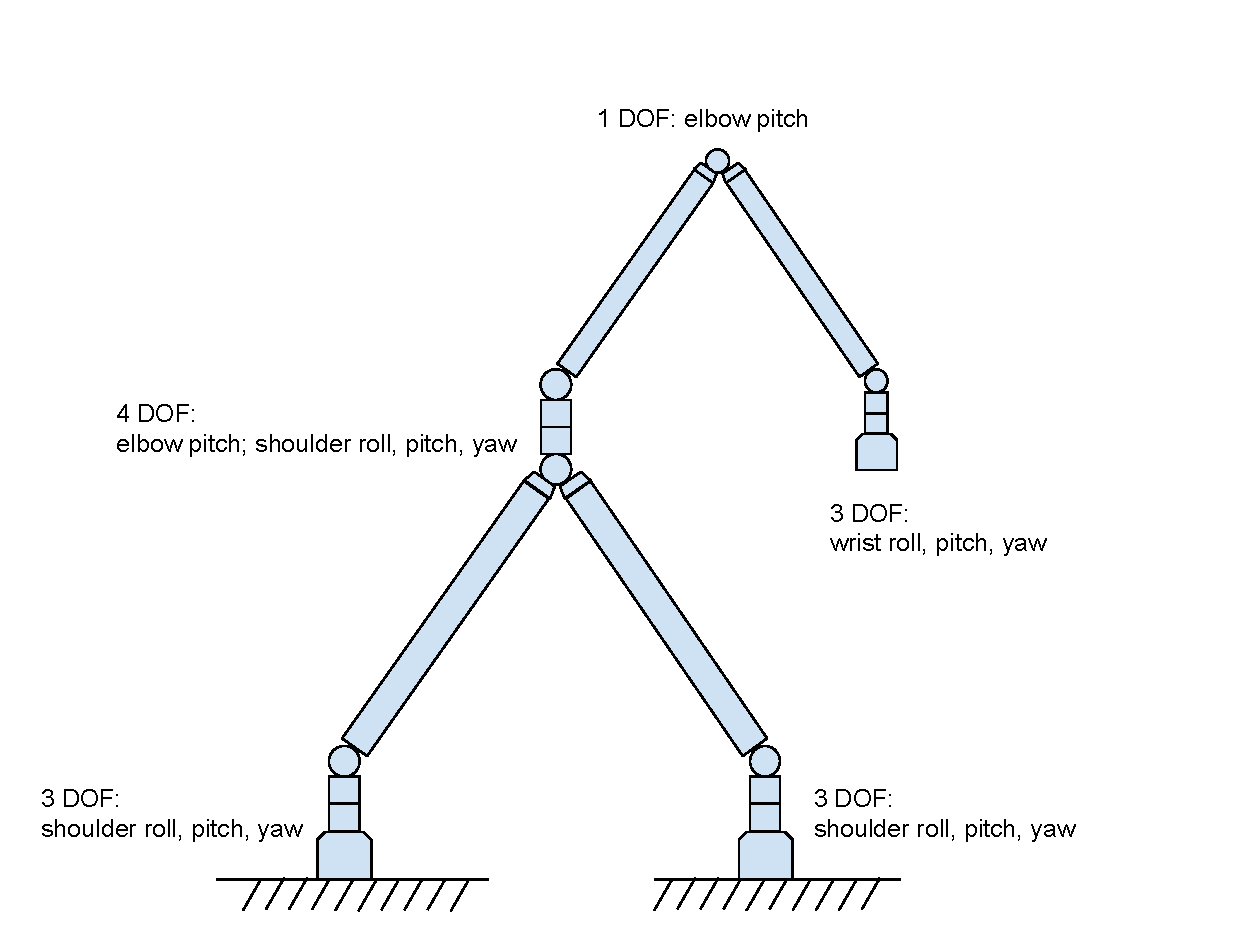
\includegraphics[width=0.5\textwidth]{14dof}
\caption{Sketch of 14DOF arm}
\label{fig:14dof}
\end{figure}
}
\item{\textbf{7 DOF robotic arm with 2 telescopic booms and 2 end effectors}\\
This architecture has two telescopic booms that would be extended once the robotic system is unstowed. The telescopic booms are extended by first connecting both end effectors on the Outpost and allowing the shoulder joint to freely rotate. Then, the elbow joint will rotate and extend the telescopic boom and two booms will extend separately.

The end effectors can grapple to Outpost to perform Outpost reconfiguration as well as free flying vehicles for capture and berthing. The end effectors can also connect to tools that are used for Outpost inspection and maintenance. The sketch of the architecture is shown in \Cref{fig:7dof} below.
\begin{figure}[H]
\centering
%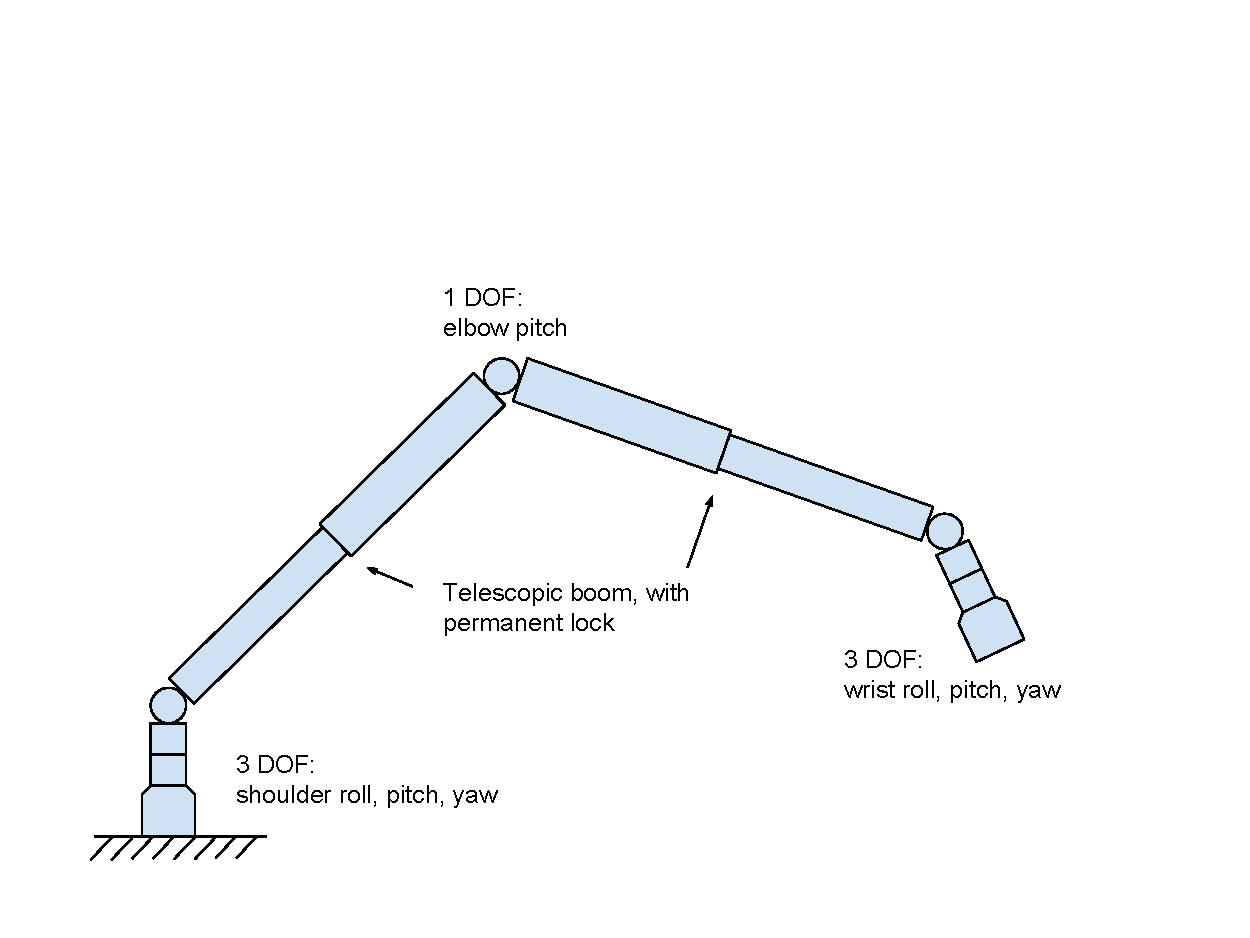
\includegraphics[width=0.55\textwidth]{7dof}
\caption{Sketch of 7DOF arm}
\label{fig:7dof}
\end{figure}
}
\item{\textbf{14 DOF robotic arm with truss rail, 2 booms and 2 end effectors}\\
As shown in \Cref{fig:14dof_truss} below, this design is composed of two parts. The first part is a 8 DOF arm with a truss rail and two booms. The end effectors can grapple to the Outpost to maneuver the robotic arm around the Outpost and perform Outpost reconfiguration. The end effectors can also grapple to free flyingr vehicles for capture and berthing operations. For inspection, maintenance and repair operations, two end effectors will be fixed on the Outpost and the truss rail between two elbow joints will act as guides for the fine arm.

The fine arm has 6 DOF and can move on the truss rail to perform inspection, maintenance and repair operations. Different tools can be attached to the end of the fine arm for specific tasks.
\begin{figure}[H]
\centering
%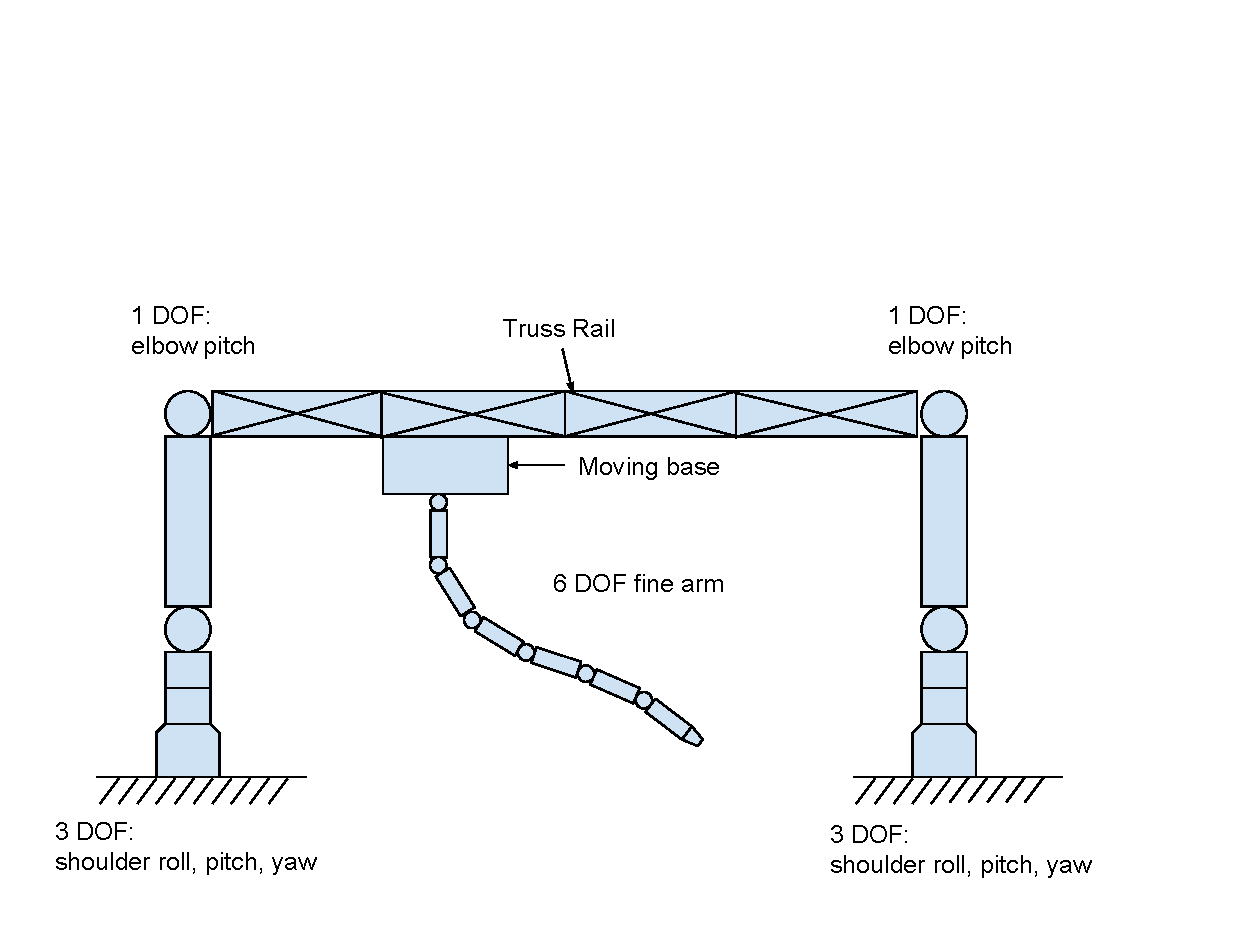
\includegraphics[width=0.6\textwidth]{14dof_truss}
\caption{Sketch of 14DOF arm with truss}
\label{fig:14dof_truss}
\end{figure}
}
\end{enumerate}

\begin{table}[H]
\centering
\caption{Trade Study of Architecture}
\begin{tabular}{|P{2.5cm}|P{4.1cm}|P{4.1cm}|P{4.0cm}|}
\hline
	&	\textbf{Architecture \#1}	&	\textbf{Architecture \#2}	&	\textbf{Architecture \#3}	\\\hhline{|=|=|=|=|}
\textbf{Structure Stability}	&
\textcolor{OliveGreen}{Robot has two fixed points on the Outpost, providing more stability}	&
\textcolor{red}{Robot has only one point fixed to the Outpost, arm will vibrate easily}	&
\textcolor{OliveGreen}{Robot has two fixed points on the Outpost, providing more stability}	\\\hline
\textbf{System Complexity}	&
\textcolor{red}{High complexity due to 14 degrees of freedom [Fund Robo]}	&
\textcolor{OliveGreen}{Lower complexity due to less degrees of freedom, heritage from Canadarm2}	&
\textcolor{red}{High complexity due to 14 degrees of freedom [Fund Robo]}	\\\hline
\textbf{Mass Required}	&
\textcolor{red}{Heaviest out of three due to 14 joints in total [That ERA thing]}	&
\textcolor{OliveGreen}{Lightest out of three\newline Least number of joints}	&
\textcolor{orange}{Medium: Has 8 joints and mechanical parts related to fine arm}	\\\hline
\textbf{Volume Occupied}	&
\textcolor{red}{Large volume due to more booms in the system}	&
\textcolor{OliveGreen}{Least volume out of three: 2 telescopic booms that are retracted in launch position}	&
\textcolor{red}{Large volume due to addition of truss and a fine arm}	\\\hline
\textbf{System Range}	&
\textcolor{orange}{Short range due to relatively shorter boom}	&
\textcolor{OliveGreen}{Long range due to telescopic boom that will extend}	&
\textcolor{orange}{Short range due to relatively shorter boom}	\\\hline
\textbf{Dexterous Tasks}	&
\textcolor{OliveGreen}{High stability due to smaller dexterous arm}	&
\textcolor{orange}{System can attach to tool for dexterous task\newline Low stability}	&
\textcolor{OliveGreen}{System has small dexterous arm\newline High stability}	\\\hline
\end{tabular}
\label{table:architectureto}
\end{table}

%----------------------------Material---------------------------
\subsubsection{Material of Frame}
\label{sect:materialto}
The material of the frame is directly related to the mass and shape of the system. Certain materials are too brittle to manufacture in desired shapes, and will aect the architecture of the system. As the material heavily aects mechanical aspects of the design, trade study on the material of frame was conducted. Material with low density, low coecient of thermal expansion, and high strength are desired for the frame of the system. Commonly used materials in the space industry include carbon bre, aluminum, stainless steel, and titanium. Each material has numerous variations with dierent properties and name. A trade study between four materials were conducted in table below.

\begin{table}[H]
\centering
\caption{Trade Study for type of Thermal Control System}
\begin{tabular}{|P{3.6cm}|P{3.1cm}|P{2.4cm}|P{2.3cm}|P{2.5cm}|}
\hline
	&	\textbf{PAN (Polyacrylonitrile) Carbon Fiber, Aerospace \cite{carbonfibreprop}}	&\textbf{Aluminium 7075 \cite{alumniumprop}}	&	\textbf{Stainless Steel 304 \cite{steelprop}}	&	\textbf{Titanium (Ti-6A/4V) \cite{titaniumprop}}	\\\hhline{|=|=|=|=|=|}
\textbf{Density (\si{\kilo\gram\per\metre\cubed})}	&	
1.8	&	2.81	&	8	&	4.43	\\\hline
\textbf{Ultimate Tensile Strength (\si{\mega\pascal})}	&
3450 to 5520	&	572	&	505	&	900 to 100	\\\hline
\textbf{Thermal Coefficient of Expansion (\si{\micro\metre\per\metre\per\kelvin})}	&	
-0.4 to -0.75	&	23.6	&	17.3	&	8.6	\\\hline
\textbf{Young's Modulus (\si{\giga\pascal})}	&
220 to 448	&	71.7	&	193 to 200	&	113.8	\\\hline
\end{tabular}
\label{table:materialto}
\end{table}

The specific properties of carbon fiber will vary with orientation and volume of the fibers and type of resin used. Aerospace grade carbon fiber, which has high stiffness to weight ratio, were selected for comparison. Other space robotic arms, such as Canadarm, Canadarm2, and ERA are made of carbon fiber as well. In general, carbon fiber is much lighter than titanium and stainless steel, have lower magnitude of thermal coefficient of expansion, and higher young’s modulus and tensile strength. Overall, aerospace grade carbon fiber is the most desirable option out of the four.

%----------------------------End Effector---------------------------
\subsubsection{End Effector}
\label{sect:endeffectorto}
In order to interact with the external subsystems situated around EML2, including the Outpost, astronauts and other modules during various operations, an end effector subsystem is required to build connections with the Outpost and other modules. And the interface established by the end effector shall capable of providing power and data connections to and from the robotic system.

As a result of those criteria, two potential end effector models are listed and compared below:

\textbf{Three fingers-three petals End Effector}: There are two main subassemblies of this end effector: an active mechanism, which consists of a motor driven lead screw that would accurate the linkages between the three finger and three petals; a passive structure, whose geometry will allow it to be constrained by the linkages and therefore establishing a rigid interface.	\\
\textbf{Steel cable-snared End Effector}: This end effector system consists of the snaring and rigidizing subassembly inside the shell, and four latch/umbilical subassemblies outside the shell, which are responsible for the rigidizing loop and the connecting loop after the fine positioning for latching and connecting operation is reached.

\begin{longtable}{|P{2.5cm}|P{6.35cm}|P{6.35cm}|}
\caption{Trade Study for type of End Effector}\\
\hline
&	\textbf{Steel cable-snared End Effector}	&	\textbf{Steel cable-snared End Effector}\\\hhline{|=|=|=|}
\endfirsthead
\hline
&	\textbf{Steel cable-snared End Effector}	&	\textbf{Steel cable-snared End Effector}\\\hhline{|=|=|=|}
\endhead
\label{longtable:endeffector}
\textbf{System Complexity}	&
\textcolor{OliveGreen}{Two main subassemblies\newline Can accomplish capturing, rigidizing and connection by only one actuator. \cite{CJME_EE}}	&
\textcolor{OliveGreen}{Two main subassemblies\newline An orbit replaceable unit, end effector can be easily replaced or repaired on orbit \cite{CJME_EE}}	\\\hline
\textbf{Operation Accuracy}	&
\textcolor{OliveGreen}{Capable of misalignment tolerance}\newline\textcolor{red}{Not suitable for soft capture \cite{CJME_EE}}	&
\textcolor{OliveGreen}{Has a strong capability of misalignment tolerance\newline Has enormous capability of soft capture \cite{CJME_EE}}	\\\hline
\textbf{Mass Required}	&
\textcolor{orange}{Maximum \SI{50}{\kilo\gram} \cite{orbital_capture}}	&
\textcolor{orange}{Maximum \SI{50}{\kilo\gram} \cite{orbital_capture}}	\\\hline
\textbf{Volume Occupied}	&
\textcolor{red}{Relatively large: maximum circumradius \SI{350}{\milli\metre} to \SI{500}{\milli\metre} \cite{CJME_EE}\cite{orbital_capture}}	&
\textcolor{OliveGreen}{Small: maximum circumradius \SI{280}{\milli\metre} \cite{CJME_EE}}	\\\hline
\textbf{Power Required}	&
\textcolor{OliveGreen}{Low, only one actuator required \cite{CJME_EE}}	&
\textcolor{OliveGreen}{Low, maximum \SI{100}{\watt} \cite{ERA_EE}}	\\\hline
\textbf{Maximum Payload}	&
\textcolor{red}{Relatively small \cite{orbital_capture}}	&
\textcolor{orange}{Large at a low speed \cite{ERA_EE}}	\\\hline
\end{longtable}

According to this comparison, the second design - Steel cable-snared End Effector is more suitable for our project. And in addition to those advantages listed, the Steel cable-snared End Effector is a proven technology, which has been applied on existing projects like the European Robotic Arm (ERA)\cite{orbital_capture}.

%----------------------------Motor---------------------------
\subsubsection{Locomotion - Motor type}
\label{motorto}
In order to efficiently navigate around the Outpost and move astronauts as well as other modules to their desired destination, a proper types of motors need to be selected for the locomotion subsystem. The chosen motor shall be able to fit in the mass/volume constraints, and shall capable of providing enough torque to the system. Three models have been considered – Stepper Motor, Brushless DC Motor and Brush DC Motor, which are compared in \Cref{table:motorto}:

\begin{table}[H]
\caption{Trade Study for Type of Motor}
\begin{tabular}{|P{2.5cm}|P{4.1cm}|P{4.1cm}|P{4.1cm}|}
\hline
	&
\textbf{Stepper Motor}	&	
\textbf{Brushless DC Motor}	&
\textbf{Brush DC Motor}	\\\hhline{|=|=|=|=|}
\textbf{Torque Capability}	&
\textcolor{orange}{High torque/power ratio at low speed and low power \cite{ESA_motor}}\newline\textcolor{red}{Short term-peak torque capability is limited by magnetic saturation\newline Low angular torque stiffness\newline  Noisy, creating significant speed ripple and microgravity disturbances \cite{ESA_motor}}	&
\textcolor{OliveGreen}{Torque/power is  high\newline Given torque can be obtained at any working speed, if power allows\newline Significant short-term peak torque capability, with a peak value which can be more than five times the nominal demand\newline Less noise\cite{ESA_motor}}	& 
\textcolor{OliveGreen}{Similar to the Brushless DC Motor, with lower power consumption \cite{ESA_motor}}\newline\textcolor{red}{Brushes have major drawbacks in space environments (i.e. disruptive voltages after a dormant period) \cite{ESA_motor}}   \\\hline
\textbf{Electric Driver Complexity}	&
\textcolor{OliveGreen}{Simplest\newline Resulting incremental stepping motion matches with many mechanisms requirements \cite{ESA_motor}}	&
\textcolor{red}{More complex than “simplest” stepper motor driver \cite{ESA_motor}}\newline\textcolor{orange}{Complexity will be reduced if a position exists in system  \cite{ESA_motor}}  & 
\textcolor{red}{Similar to the brushless DC motor \cite{ESA_motor}} 	\\\hline
\textbf{Mass/ Volume Required}	&
\textcolor{OliveGreen}{Usually does not require a dedicated position sensor \cite{ESA_motor}}	&
\textcolor{red}{Always needs a position sensor \cite{ESA_motor}}   & 
\textcolor{OliveGreen}{Mass/size is relatively smaller than brushless DC Motor\cite{ESA_motor}}	\\\hline

\textbf{Life Expectancy}	&
\textcolor{OliveGreen}{\textgreater10000 hours \cite{Pittman_motor}}	&
\textcolor{OliveGreen}{\textgreater10000 hours \cite{Pittman_motor}}   & 
\textcolor{red}{2000 to 5000 hours \cite{Pittman_motor}}	\\\hline
\end{tabular}
\label{table:motorto}
\end{table}
From the trade study, the brushless DC motor has a better performance than the other two compared models, and has a significant advantage at the torque capability. Also, brushless DC motor has been considered for previous space arm robot project \cite{ERA_motor}, which will decrease its development risk. Therefore, a brushless DC motor is chosen to be used on the locomotion subsystem.

%----------------------------Joint---------------------------
\subsubsection{Locomotion - Joint type}
\label{sect:jointto}
As a major part of the locomotion subsystem, the joints utilize rotation of the motors to accomplish the motion of robotic arm. Two different joint structures that used in reference designs are inline joint and offset joint. Inline joint is used in European Robotic Arm and offset joint is used in Canadarm2. Depend on the tasks that two arms need to perform, both joint structures have advantages and disadvantages.
\begin{table}[H]
\caption{Trade Study for type of Joint}
\begin{tabular}{|P{2.5cm}|P{6.35cm}|P{6.35cm}|}
\hline
	&	\textbf{Inline Joint}	&
	\textbf{Offset Joint}	\\\hhline{|=|=|=|}
\textbf{Operation Complexity}	&
\textcolor{OliveGreen}{No joint collision risk, components are in the same plane.}	&
\textcolor{red}{Add complexity to task due to possibility of joint collision [comp]}	\\\hline
\textbf{Operation Range}	&
\textcolor{red}{Limited mobility; limited motor rotational range.}	&
\textcolor{OliveGreen}{The arm can maneuver more readily over large areas by “stepping over the elbow”; large motor rotational range[comp]}	\\\hline
\end{tabular}
\label{table:jointto}
\end{table}

The major task for Canadarm2 was to assemble the ISS. By having offset joints, the joint can rotate in larger range and enable the arm to have more flexible motion. \Cref{tab:jointrange} in \Cref{app:jointrange} shows the joint motion range for Canadarm2 and ERA \cite{arm_comp}. As the robotic system on the Outpost needs to perform reconfiguration operation, it is important to have large range of motion to maneuver the Outpost module. Therefore the offset joint structure is chosen for the locomotion subsystem.

\subsection{Electrical Trade Studies}
\label{sect:elec_to}
% Done
\subsection{Electrical Trade Studies}
\label{subsec:Electrical Trade Studies}
%----------------------------Power Storage------------------------------
\subsubsection{Power Storage}
\label{sect:powerto}
In order to provide the robotic system with power to run during contingencies, a power storage subsystem is required. A trade study of the two most commonly used rechargeable batteries in space, Li-ion and NiH$_2$ batteries,
 is conducted in \Cref{table:powerto}.
\begin{table}[H]
\centering
\caption{Trade Study for type of Power Storage}
\begin{tabular}{|P{6cm}|P{4.2cm}|P{4.2cm}|}
\hline
	&	\textbf{Li-ion}	&	\textbf{Ni-H}	\\\hhline{|=|=|=|}
\textbf{Used in}	&
Mars Rovers: Spirit \& Opportunity \cite{Liion_Mars}	&
International Space Station \cite{ISS_power}	\\\hline
\textbf{Specific Energy (Wh/kg)}	&
\textcolor{OliveGreen}{150 \cite{batt_primer}}	&	
\textcolor{red}{65 \cite{NiH_se}}	\\\hline
\textbf{Energy Density (Wh/L)}	&
\textcolor{OliveGreen}{400 \cite{batt_primer}}	&	
\textcolor{red}{10-80 \cite{NASA_energy}}	\\\hline
\textbf{Cycle Durability}	&
\textcolor{red}{1000 \cite{batt_primer}}	&	
\textcolor{OliveGreen}{\textgreater50000 \cite{NASA_energy}}	\\\hline
\textbf{Operable Temperature (\si{\degreeCelsius})}	&
\textcolor{OliveGreen}{-20 to 60 \cite{batt_primer}}	&	
\textcolor{red}{-5 to 30 \cite{NASA_energy}}	\\\hline
\textbf{Lifespan (years)}	&
\textcolor{red}{\textgreater2 \cite{NASA_energy}}	&	
\textcolor{OliveGreen}{\textgreater10 \cite{NASA_energy}}	\\\hline
\end{tabular}
\label{table:powerto}
\end{table}
Li-ion batteries are choosen since they are able to provide much more energy with a smaller mass and volume than NiH$_2$ batteries. Li-ion batteries are also operable over a much larger temperature range than NiH$_2$ batteries. Although Li-ion batteries can endure much less charge cycles than NiH$_2$, this would not be a huge problem as the batteries will only be used in contingencies, and will not be subjected to discharging and recharging on a frequent basis. The most major drawback related to the use of Li-ion batteries is the short life span, which would mean that it has to be replaced fairly frequently.

%----------------------------Thermal Control------------------------------
\subsubsection{Type of Thermal Control System}
\label{sect:thermal_to}
A trade study on the type of active thermal control system (ACTS) is made for the thermal control subsystem. Types of ATCS include electrically controlled patch heaters, fluid loop system, and louvers: patch heaters consists of an electrical-resistance material between two insulating materials; fluid loop system consists of multiple pipes and pumps and liquid material; and louvers are window shutters with adjustable angle to control heat transfer on the surface.  A trade study was conducted between the three options in \Cref{tab:thermalto}.

\begin{table}[H]
\centering
\caption{Trade Study on type of ATCS}
\begin{tabular}{|P{3.3cm}|P{3.8cm}|P{3.8cm}|P{3.8cm}|}
\hline
	&	\textbf{Patch Heater\cite{heater_design}\cite{flex_heater}}	&
\textbf{Fluid Loop\cite{mech_fluidloop}\cite{hightemp_fluidloop}}	&
\textbf{Louvers \cite{tc_tech}}	\\\hhline{|=|=|=|=|}
\textbf{Implementation}	&	
\textcolor{OliveGreen}{Only require cables to transmit electricity and patch heaters to be placed at various positions to heat the system}	&	
\textcolor{red}{Very difficult to store cables, pumps and valves for moving parts}	&	
\textcolor{OliveGreen}{Easy to install on surface}	\\\hline
\textbf{System Complexity}	&	
\textcolor{OliveGreen}{Each patch heater is a thin foil\newline Little to no mechanical parts}	&	
\textcolor{red}{Various pumps, valves and pipes to carry fluid are needed}	&
\textcolor{orange}{Located on the surface of the system\newline Physically alters shape of system}	\\\hline
\textbf{Power Consumption}	&	
\textcolor{orange}{Dependent on area needed to be heated, approximately \SI{5}{\watt\per\square{in}}}	&
\textcolor{red}{\textless\SI{150}{\watt} for CFC-11 (Exact numbers can vary to up to \SI{14}{\kilo\watt} depending on fluids used)}	&
\textcolor{orange}{Medium power consumption used to drive the movement of the louvers}	\\\hline
\textbf{System Reliability}	&	
\textcolor{orange}{Large operational range, area is limited to number of active units}	&
\textcolor{OliveGreen}{Fluid loop covers larger region of the system}	&
\textcolor{red}{System heats up from exposure to sunlight\newline Louvers do not heat up system when there is no sunlight}	\\\hline
\textbf{System Mass}	&
\textcolor{OliveGreen}{\textless\SI{0.1}{\kilo\gram} for standard patch heaters}	&
\textcolor{red}{\textless\SI{25}{\kilo\gram}, excluding fluid and radiators}	&
\textcolor{orange}{Medium, mostly mass of motors needed to drive louvers}	\\\hline
\end{tabular}
\label{tab:thermalto}
\end{table}
The main drivers behind the decision were reliability and implementation of the ACTS. Louvers, by itself, does not control the temperature of the system. It only adjusts amount of sunlight exposed to the system, and cannot control the temperature when the system is not exposed to sunlight\cite{tc_tech}. Therefore, two other systems are more reliable.

Out of three options, the fluid loop is most difficult to implement. Furthermore, the mass budget of the thermal control system is \SI{12.6}{\kilo\gram} with 30\% mass margin. Trying to implement fluid loop heater with this constraint would be time consuming and costly.

By comparison, patch heaters are much lighter and simpler. The level of tolerance can be increased simply by increasing number of patches and wires, which does not have significant impact on mass or power budget.

While the exact numbers vary, patch heaters consume approximately \SI{5}{\watt\per\square{in}} of patch and fluid loops consume more than \SI{150}{\watt}. The total power consumption is dependent on the size of the area of interest. 

Based on our power budget in \Cref{sect:power}, up to 28 patch heaters can be active during peak. Therefore, at all times, the heating area on the surface is limited to \SI{28}{\square{in}}, or \SI{180.645}{\square\centi\metre}. By selectively heating colder areas, it is possible to maintain the temperature of subsystems in operable range.  Assuming passive thermal blanket covers the system, the heat generated from patches will remain in the system. The combination of patches and radiator can maintain the temperature of subsystems by selectively and cyclically heating colder areas. Moreover, it is possible to heat wider surface at cost of less voltage. Further research needs to be done on choosing which units to activate and calculating optimum duration of heating per unit. Polyamide patch heaters have temperature range of \SI{-200}{\degreeCelsius} to \SI{150}{\degreeCelsius}, which covers operational range of all subsystems \cite{heater_design}.

%----------------------------Network Topology------------------------------
\subsubsection{Type of Network Topology}
\label{sect:network_to}
The network topology used is directly related to the transfer of data across the different subsystems. A trade study on four common network topologies that can be used (bus, mesh, ring and star) was conducted in \Cref{tab:networkto}.

A bus topology uses a common backbone to connect all nodes in the system. There is a direct link between the backbone and each node. 

A mesh topology has every node connected to each other in a complex network of cables. Data can take one of several different paths between two nodes.

A ring topology has every node connected to two other nodes. All data travels in one direction in a ring.

A star topology has every node connected directly to a central hub, with no connections between individual nodes.
\begin{table}[H]
\centering
\caption[Trade Study on type of Network Topology]{Trade Study on type of Network Topology\cite{studytopology}\cite{topology_intro}}
\begin{tabular}{|P{2.5cm}|P{3cm}|P{3cm}|P{3cm}|P{2.9cm}|}
\hline
	&	\textbf{Bus}	&	\textbf{Mesh}	&	\textbf{Ring}	&	\textbf{Star}	\\\hhline{|=|=|=|=|=|}
\textbf{Mass of System}	&
\textcolor{OliveGreen}{Only main backbone and a cable connecting backbone to each node}	&
\textcolor{red}{Many cables required to connect all nodes to each other}	&
\textcolor{orange}{Requires cables to form a ring around all nodes}	&
\textcolor{orange}{Requires cables to run across entire distance between central hub and nodes}	\\\hline
\textbf{Single Fault Tolerance}	&
\textcolor{orange}{Network fails if failure happens on backbone}	&
\textcolor{OliveGreen}{Even if one connection fails, other connections remain intact}	&
\textcolor{red}{Entire network fails if a single node or connection fails}	&
\textcolor{orange}{Network fails if central hub fails}	\\\hline
\textbf{System Complexity}	&
\textcolor{OliveGreen}{Main connection is single backbone with single connections to each node}	&
\textcolor{red}{Every node needs to connect to every other node}	&
\textcolor{OliveGreen}{Each node only connects to following and previous node}	&
\textcolor{OliveGreen}{Each node is only connected to a central hub directly}	\\\hline
\textbf{Ease of debugging}	&
\textcolor{red}{Difficult to pinpoint location of faults in system}	&
\textcolor{red}{Difficult to pinpoint location of faults in system}	&	
\textcolor{OliveGreen}{Easy to pinpoint location of faults in system}	&	
\textcolor{OliveGreen}{Easy to pinpoint location of faults in system}	\\\hline
\textbf{Ease of adding new nodes}	&
\textcolor{OliveGreen}{Easy to add new nodes to backbone, only one connection to backbone required}	&
\textcolor{red}{Needs to add connections from new node to every other node, can be complicated for large systems}	&
\textcolor{red}{Difficult to add new nodes, need to remove and add connections to two nodes}	&
\textcolor{OliveGreen}{Easy to add new nodes as only a single connection to central hub needs to be made}	\\\hline
\end{tabular}
\label{tab:networkto}
\end{table}
Since the mass of the system is one of our drivers and the system is required to be single fault tolerant, these are the two most important considerations in our trade study. A bus topology will minimize the mass spent on cables due to needing only a single backbone while star topology is slightly higher as cables are needed to be laid for the entire length between different subsystems. Although both topologies are not single fault tolerant, it is relatively simple to implement a duplicate bus to allow for single fault tolerance in a bus topology whereas adding an additional set of cables as redundancy would result in excessive cables in the system, adding to system complexity. There is also relatively low complexity in a bus topology, although debugging would take a longer time due to the relatively higher difficulty in locating faults in the bus. However, time spent in debugging could easily be traded off as the bus topology will best satisfy our drivers and requirements.

%----------------------------Data Comm------------------------------
\subsubsection{Type of Data Communication System - Wired vs. Wireless}
\label{sect:datacomm_to}
For communication between the robot system and the Outpost, a trade-off study comparing a wire-based communication system and a wireless communication system is shown in \Cref{tab:datacommto}.
\begin{table}[H]
\caption{Trade Study for Type of Thermal Control System}
\begin{tabular}{|P{3.5cm}|P{5.8cm}|P{5.8cm}|}
\hline
	&	\textbf{Wire-based Communication System}	&	\textbf{Wireless Communication System}	\\\hhline{|=|=|=|}
\textbf{Communication speed}	&
\textcolor{OliveGreen}{Can provide both low and high-speed communication (between 2 and 400 \si{\mega bps}) \cite{spacewire_comm}}	&
\textcolor{OliveGreen}{Capable of providing high-speed data transformation \cite{CCSDS_design}}	\\\hline
\textbf{System Complexity}	&
\textcolor{red}{Entire system consists of connectors, cables, cable assemblies and printed circuit board tracks \cite{spacewire_comm}}	&
\textcolor{OliveGreen}{No need for cable planning and assembly \cite{CCSDS_design}}	\\\hline
\textbf{Mass/Volume Occupation}	&
\textcolor{red}{Connectors and cable assemblies will add to the weight and volume of the whole system \cite{spacewire_comm}}	&
\textcolor{OliveGreen}{Does not require components like cable assemblies}	\\\hline
\textbf{Technology Availability}	&
\textcolor{OliveGreen}{Do not require much technological support. For example, SpaceWire has been used on many previous space missions \cite{spacewire_uses}}	&
\textcolor{OliveGreen}{Has been previously used on ISS, for example, Space-to-Space Station Radio (SSSR) \cite{commtracksys}}	\\\hline
\end{tabular}
\label{tab:datacommto}
\end{table}
According to the table, a wireless communication system has more advantages compared to a wire-based communication system. It requires less mass and volume, which satisfies the major drivers of this project.

%----------------------------Redundancy------------------------------
\subsubsection{Type of Redundancy in System}
\label{sect:redundancy_to}
In the RFP, the system is required to be single fault tolerant. This requires the system to have redundancy built in. Similar to the Canadarm2 and ERA, the robotic system will has a redundant electrical systems to assure single fault tolerance. Each sub-unit in the electrical system has a redundant backup unit, and the primary/redundant systems are both fully capable of performing the electrical functions \cite{ISS_robotcompare}. The redundancy in the electrical system will increase the mass; however, the mass of electrical system is relatively light \cite{AER407_Mech}, justifying the use of such redundancy.

There are two ways to implement the redundant system: cross strapped architecture and separate architecture. Cross strapped architecture has a unit that connects to both primary and redundant systems, whereas in a separate architecture , there is no connection between primary and redundant system. The architectures are shown in \Cref{fig:redundancy}. The trade study for these two architectures is shown in \Cref{tab:redundancyto}.

\begin{figure}[H]
\centering
\begin{subfigure}[H]{0.5\textwidth}
%\includegraphics[height=115pt]{nocrossstrap}
\end{subfigure}
\hfill
\begin{subfigure}[H]{0.45\textwidth}
%\includegraphics[height=115pt]{yescrossstrap}
\end{subfigure}
\caption[Separate Architecture and Cross-strapped Architecture]{Separate Architecture and Cross-strapped Architecture \cite{AER407_ElectricalPresentation}}
\label{fig:redundancy}
\end{figure}

\begin{table}[H]
\centering
\caption{Trade Study for Type of Redundancy Architecture}
\begin{tabular}{|P{3cm}|P{5.5cm}|P{5.5cm}|}
\hline
	&	\textbf{Cross Strapped}	&	\textbf{Separate}	\\\hhline{|=|=|=|}
\textbf{System Reliability}	&
\textcolor{red}{Used in both primary and redundancy systems, leading to lower mean time to failure of entire system \cite{AER407_electricalnotes}}	&
\textcolor{OliveGreen}{Redundant system is separate and used only when primary system fails, leading to higher reliability}	\\\hline
\textbf{System Availability}	&
\textcolor{OliveGreen}{Can operate in both primary and redundancy systems without reconfiguration \cite{ISS_robotcompare}}	&
\textcolor{red}{Time gap to switch to redundant system when primary system fails}	\\\hline
\textbf{System Complexity}	&
\textcolor{red}{High complexity with complex failure mode analysis \cite{spacecraftdesign}}	&
\textcolor{OliveGreen}{Low complexity}	\\\hline
\textbf{Single Fault Point}	&
\textcolor{red}{Adds single point failure modes \cite{AER407_electricalnotes}}	&
\textcolor{OliveGreen}{No single point failure mode}	\\\hline
\end{tabular}
\label{tab:redundancyto}
\end{table}
The separate architecture has the advantage of higher reliability and no single point failure mode; the cross strapped architecture has the advantage of higher reliability. For the thermal control units, which include heaters and heater controllers, the cross strapped architecture is used to keep the robotic system at survival temperature range during the system switching if the primary system is failed. However, to achieve single fault tolerance, there are redundancies built within the thermal control units. There are four heaters connected in parallel so that if one fails the other will continue working, and the thermal controller will also have redundancy.

Another unit that is cross strapped is the Camera and Lighting Unit (CLU) that includes camera, video frame grabber and light. The cameras are used to assist free flyer capture and berthing, the positions of the cameras are fixed for video reference. Thus there will be no redundancy for the cameras and the CLU is cross strapped to both primary and redundant system. However, CLU has built in redundancy for video frame grabbers.

The rest of the system has separate architecture redundancy since it has lower complexity, higher reliability and no single point failure mode. 


\subsection{Controls Trade Studies}
\label{sect:ctrl_to}
\subsection{Control Trade Studies}


%--------------Architecture
\newpage
\section{System Architecture}
\subsection{Mechanical Architecture}
\subsection{Electrical Architecture}
\subsection{Control Architecture}

%--------------Detailed Design
\newpage
\section{Detailed Design}
\subsection{Mechanical Design}
\subsection{Electrical Design}
\subsection{Control Design}

%--------------Budget
\newpage
\section{Budget}
\label{sect:budgets}
\subsection{Mass Budget}
\label{sect:massbudget}
Mass budget comes here
%\begin{table}[H]
%\centering
%\caption{Mass Budget}
%\begin{tabular}{C{4cm}C{2cm}C{2cm}C{2cm}C{2cm}}
%\toprule
%\textbf{Subsystem}	&	\textbf{Allowed Mass(kg)}	&	\textbf{Percentage}	&	\textbf{Margin}	&	\textbf{Allocated Mass(kg)}\\\midrule
%\textbf{Locomotion}						
%&	146.6	&	42.5\%	&	30\%	&	190.58	\\
%\textbf{Data Handling \& Processing}	
%&	13.8	&	4\%		&	30\%	&	17.94	\\
%\textbf{Thermal Control}				
%&	3.5		&	1\%		&	30\%	&	4.55	\\
%\textbf{Power}							
%&	6.9		&	2\%		&	30\%	&	8.97	\\
%\textbf{End Effector}					
%&	100		&	29\%	&	30\%	&	130	\\
%\textbf{Sensors}						
%&	5.2		&	1.5\%	&	30\%	&	6.76	\\
%\textbf{Frame}							
%&	34.5	&	10\%	&	30\%	&	44.85	\\
%\textbf{Cables}							
%&	34.5	&	10\%	&	30\%	&	44.85	\\\hline
%\textbf{Total}	&	\textbf{345}	&	\textbf{100\%}	&	\textbf{30\%}	&	\textbf{448.5}\\\bottomrule
%\end{tabular}
%\label{tab:mass}
%\end{table}
\subsection{Power Budget}
\label{sect:powerbudget}
\subsubsection{Average Power Budget}
Average Power Budget

\subsubsection{Peak Power Budget}
Peak Power Budget


%--------------Conclusion
\newpage
\section{Conclusion}
\label{sect:Conclusion}

%--------------------------------------------------------------------------------------------------------------------------------------------------------------------------------
\newpage
\bibliographystyle{unsrt}
\bibliography{reportbib}

\newpage
\appendix
\section{Load Calculations}
\label{app:loadcalc}
\setcounter{equation}{0}
At \gls{EML2}, the gravitational acceleration is nearly zero, the force acting on the arm is coming from external contact like \gls{EVA} or the acceleration of payload.

\large \textbf{Payload reaction force/torque}\\
\normalsize There is no moving speed and stopping distance requirement proposed by customer. However, we can use the performance of reference design such as Canadarm and Canadarm2 to calculate a reference loading requirement. 

Tip velocity of Canadarm with full payload:$v=\SI{0.06}{\metre/\second}$\\
Canadarm stopping distance with full payload: $b=\SI{0.6}{\metre}$\\
Leaving a 30\% margin, Stopping Distance: $b=\SI{0.42}{\metre}$\\
Maximum payload mass from \gls{RFP}: $m=\SI{10000}{\kilo\gram}$

Assume payload acceleration is constant, the following two equations are used to calculate acceleration:
\begin{equation}
b=v_it+\frac{1}{2}at^2
\end{equation}
\begin{equation}
a=\frac{v_f-v_i}{t}
\end{equation}
where:\\
$v_i=v$ is the initial velocity of payload\\
$v_f=0$ is the final velocity of payload\\
This gives us a result of $$t=\SI{14}{\second}, a=\SI{0.0043}{\metre/\square\second}$$

The reaction force applied by the payload is 
$$F=ma=\SI{10000}{\kilo\gram}\times\SI{0.0043}{\metre/\square\second}=\SI{43}{\newton}$$

This reaction force will apply a bending moment to the robotic arm. Another type of load applied by the payload is torque due to the rotational motion. Canadarm2's rotational velocity and stopping angle are used. 

Rotational Velocity: $\omega=\SI{0.24}{\degree/\second}=\SI{0.0042}{rad/\second}$ \cite{NASAsysreq_Kumar}\\
Rotational Stopping Distance: $\theta=\SI{3.8}{\degree}$
Leaving a 30\% margin, Stopping Distance: $\theta=\SI{2.9}{\degree}=\SI{0.051}{\radian}$

These two performance characteristics of Canadarm2 are associated with payload that has mass of 209000 \gls{kg} and size of 4.5 \gls{m} in diameter and 17 \gls{m} in length. This mass is twice of the maximum required in \gls{RFP} and the size of the payload was not specified in the \gls{RFP}. The size of the payload handled by the robotic system is assumed half the length of Canadarm2 payload. This size is also a close resemblance of a service module on \gls{ISS} \cite{ISS_Harmony}.

Maximum payload mass from \gls{RFP}: $m=\SI{10000}{\kilo\gram}$
Payload size: diameter $d=\SI{4.5}{\metre}$; length $l=\SI{8.5}{\metre}$
Assume payload has uniform density, payload moment of inertia:
$$I=\frac{1}{4}m(\frac{d}{2})^2+\frac{1}{2}ml^2=\SI{253490}{\kilo\gram\square\metre}$$
The axis for the moment of inertia is chosen according to the location of the grapple fixture on the \gls{ISS} module\cite{ISS_Harmony}. The axis is marked as a black dotted line in \Cref{fig:harmony_axis}.

\begin{figure}[H]
\centering
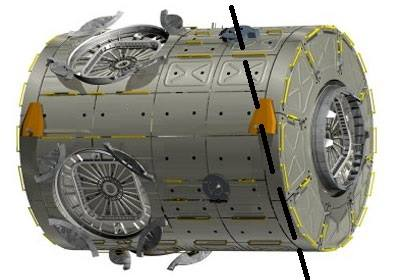
\includegraphics[width=0.4\textwidth]{Apppic/harmony}
\caption{Axis used to calculate moment of inertia}
\label{fig:harmony_axis}
\end{figure}

Assuming payload rotational acceleration is constant, the following two equations are used to calculate rotational acceleration.
\begin{equation}
\theta=\omega_it+\frac{1}{2}\alpha t^2
\end{equation}
\begin{equation}
\alpha=\frac{(\omega_f-\omega_i)}{t}
\end{equation}
where:\\
$\omega_i=\omega$ is the initial rotational velocity of payload\\
$\omega_f=0$ is the final rotational velocity of payload

This gives us the result of $$t=\SI{24}{\second}, \alpha=\SI{0.00177}{\radian/\square\second}$$
The reaction torque applied by the payload is then
$$\tau=I\alpha=\SI{253490}{\kilo\gram\square\metre}\times \SI{0.00177}{\radian/\square\second}=\SI{448.7}{\newton\metre}$$

\large \textbf{Holding/Reaction forces}\\
\normalsize Requirement \textbf{EE-P-02} states that the end effector subsystem shall apply holding or reaction forces of \SI{200}{\newton} in any direction.

\large \textbf{Holding/Reaction forces}\\
\normalsize The robotic arm can be modeled as a cantilever beam and the highest load occurs when the arm is straight as shown in \Cref{fig:loading} below. The holding and reaction force is higher than the payload reaction force, therefore the force of 200 \gls{N} from holding and reaction is used.

\begin{figure}[H]
\centering
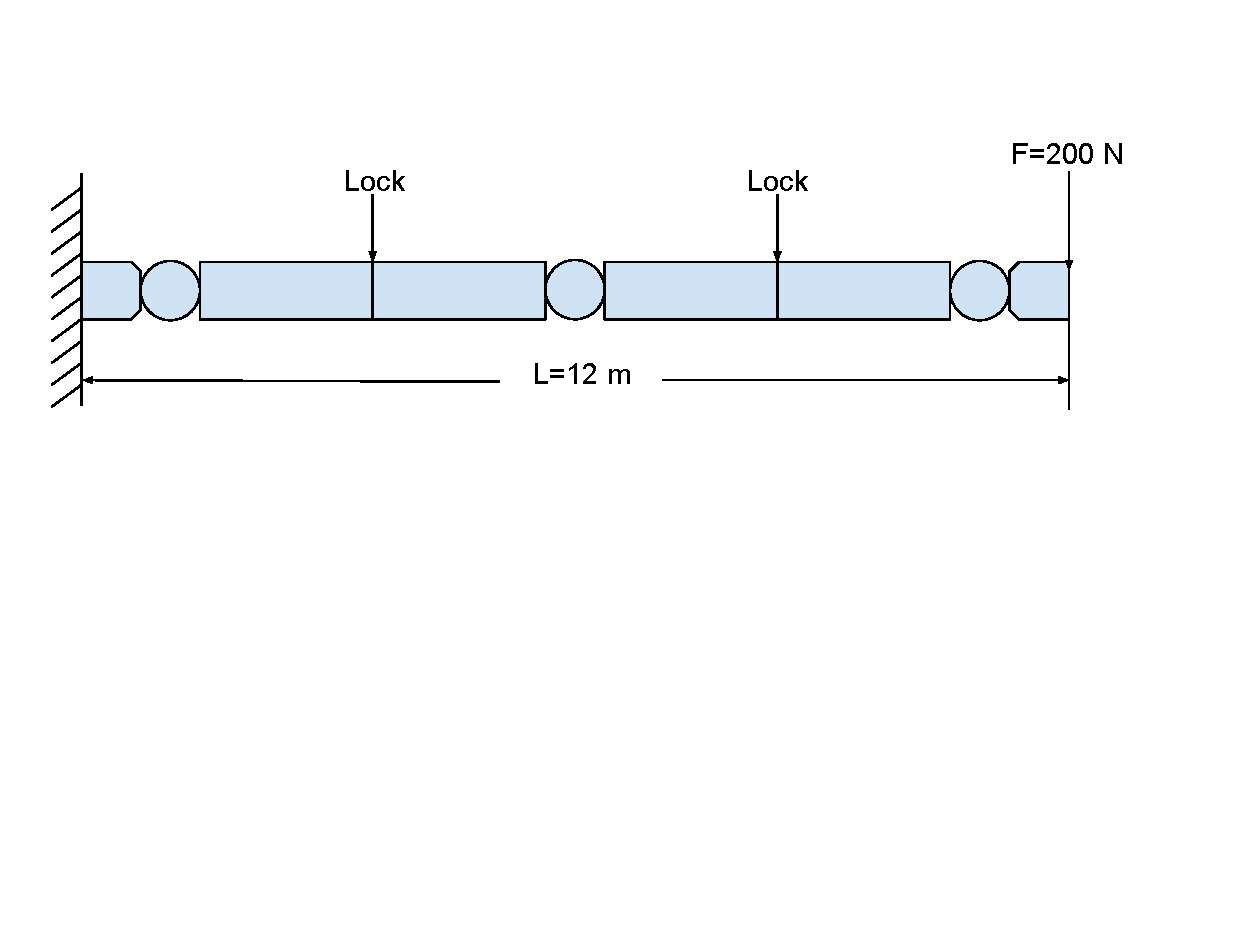
\includegraphics[width=0.6\textwidth]{Apppic/loading}
\caption{Maximum loading configuration of system}
\label{fig:loading}
\end{figure}

The maximum moment is at the end effector and shoulder joint.
$$M=FL=\SI{2400}{\newton\metre}$$
The moment at the lock where the telescopic boom is locked is:
$$M_{Lock} = FL_{Lock} = \SI{1800}{\newton\metre}$$
The moment at the elbow joint is:
$$M_{elbow} = FL_{elbow} = \SI{1200}{\newton\metre}$$
Given factor of safety of 1.5, the final bending moments on the arm are:
$$M=\SI{3600}{\newton\metre}, M_{Lock}=\SI{2700}{\newton\metre}, M_{elbow}=\SI{1800}{\newton\metre}$$
The rotational torque load on the arm is:
$$T = \SI{448.7}{\newton\metre}\cdot1.5=\SI{673.05}{\newton\metre}$$

\large \textbf{Other reference load requirement}\\
\normalsize \textbf{End Effector}\\
The end effectors of Canadarm2 need to perform snare, rigidize and latch mechanism, the load transfer capability of the end effector are \cite{NASAsysreq_Kumar}:\\
i) ``950 \gls{Nm} torque and 1220 \gls{Nm} bending moment when snared and rigidized, allowing \SI{3}{\degree} separation at the interface."\\
ii) ``3210 \gls{Nm} moment about any axis and 1110 \gls{Nm} axial/shear force when snared, rigidized and latched and no separation at the interface"

\textbf{Vibrational Load}\\
During the launch of the aircraft, the robotic system will experience vibrational load and shock load due to engine firing and engine cut off. While the type of the launch vehicle is specified in \gls{RFP}, the common launch vehicles used are Atlas V and Delta IV, and design characteristics use these vehicles. The vibration design, shock design and testing characteristics are presented in \Cref{delta_launch,atlas_launch} below

\begin{table}[H]
\centering
\caption[Vibration design, shock design and testing characteristics of Delta IV]{Vibration design, shock design and testing characteristics of Delta IV \cite{delta_launch}}
\begin{tabular}{|c|c|c|c|}
\hline
	&	\textbf{Frequency (\gls{Hz})}	&	\textbf{Test Level}	&	\textbf{Sweep Rate}	\\\hhline{|=|=|=|=|}
{\textbf{Sinusoidal Vibration}}	&	5 to 7.4	&	1.27 \gls{cm} double amplitude	&	\multirow{2}{*}{2 octaves/min}	\\\cline{2-3}
{\textbf{Axial}}	&	7.4 to 100	&	1.4 \gls{g} (zero to peak)	&	\\\hline
{\textbf{Sinusoidal Vibration}}	&	5 to 6.2	&	1.27 \gls{cm} double amplitude	&	\multirow{2}{*}{2 octaves/min}	\\\cline{2-3}
{\textbf{Lateral}}	&	6.2 to 100	&	1.0 \gls{g} (zero to peak)	&	\\\hline
\textbf{Shock}	&	150	&	120 \gls{g}	&	N/A	\\\hline

\end{tabular}
\label{delta_launch}
\end{table}

\begin{table}[H]
\centering
\caption[Vibration design, shock design and testing characteristics of Atlas V]{Vibration design, shock design and testing characteristics of Atlas V \cite{atlas_launch}}
\begin{tabular}{|c|c|c|c|}
\hline
	&	\textbf{Frequency (Hz)}	&	\textbf{Test Level}	&	\textbf{Sweep Rate}	\\\hhline{|=|=|=|=|}
{\textbf{Sinusoidal Vibration}}	&	\multirow{2}{*}{5 to 100}	&	\multirow{2}{*}{1.125 \gls{g} (zero to peak)}	&	\multirow{2}{*}{2 octaves/min}	\\
{\textbf{Axial}}	&		&		&	\\\hline
{\textbf{Sinusoidal Vibration}}	&	\multirow{2}{*}{5 to 100}	&	\multirow{2}{*}{0.75 \gls{g} (zero to peak)}	&	\multirow{2}{*}{2 octaves/min}	\\
{\textbf{Axial}}	&		&		&	\\\hline
\textbf{Shock}	&	270	&	120 \gls{g}	&	N/A	\\\hline
\end{tabular}
\label{atlas_launch}
\end{table}




\section{Transmitting Frequencies of Subsystems}
\label{app:frequencies}
\begin{table}[H]
\caption{Frequencies of Subsystems}
\centering
\begin{tabular}{cc}
\toprule
\textbf{Component}	&	\textbf{Frequency of communication with DH (\si{\hertz})}	\\
\midrule
\textbf{Motor/Brake Drive Amplifier}	&	20 \cite{ERA_jointctrl}			\\
\textbf{Resolvers}						&	300 \cite{ERA_jointctrl}		\\
\textbf{Camera}							&	20 \cite{MSSS_cameras}			\\
\textbf{Proximity Sensor}				&	16500 \cite{highres_proxsensor}	\\
\textbf{Force Sensor}					&	1000 \cite{ATI_forcesensor}		\\
\textbf{Torque Sensor}					&	1000\cite{Honeywell_torquesensor}\\
\textbf{Thermocouple}					&	35 \cite{temp_sensors}			\\
\bottomrule
\end{tabular}
\end{table}
The rate of data transfer between DH and Outpost/Transport Vehicle is typically between \SI{1}{\hertz} to \SI{12.5}{\hertz}. For this robotic system, it can be reasonably assumed that data will be recorded at a rate of \SI{1}{\hertz}, with the possibility of obtaining the most updated data from DH when desired \cite{ERA_collisionprevent}\cite{Space_teleop_robot}. The only exception is the \gls{CLU}, where the video feedback to the outpost will be about \SI{20}{\hertz} \cite{MSSS_cameras}.

\section{Temperature Range of Components}
\label{app:optemp}
\begin{table}[H]
\caption[Operational and Survival Temperature Ranges of various Components]{Operational and Survival Temperature Ranges of various Components \cite{NASAsysreq_Kumar}}
\centering
\begin{tabular}{|l|l|l|}
\hline
\textbf{Component}	&	\textbf{Operational (\si{\degreeCelsius})}	&	\textbf{Survival (\si{\degreeCelsius})}\\\hhline{|=|=|=|}
\textbf{Gears \& Bearings}		&	-25 to 135	&	-50 to 155	\\\hline
\textbf{Motor Windings}			&	-25 to 180	&	-50 to 200	\\\hline
\textbf{Brakes}					&	-25 to 99	&	-50 to 120	\\\hline
\textbf{Cables \& Connectors}	&	-70 to 135	&	-90 to 155	\\\hline
\textbf{Electronics}			&	-20 to 65	&	-50 to 85	\\\hline
\end{tabular}
\end{table}

\subsection*{Data from External Documents}
\begin{figure}[H]
\centering
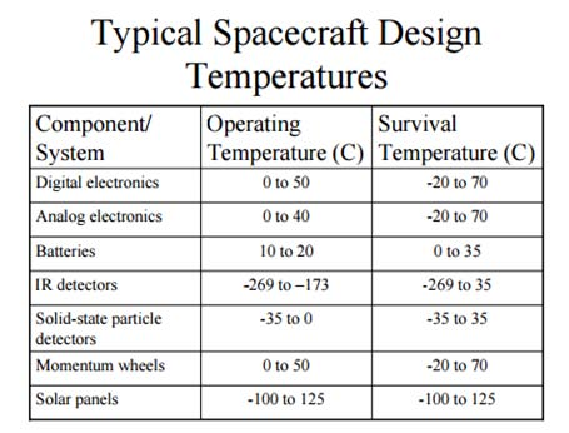
\includegraphics[scale=0.6]{Apppic/designtemp}
\caption[Typical Spacecraft Design Temperatures]{Typical Spacecraft Design Temperatures \cite{spacedesigntemp}}
\end{figure}
\begin{figure}[H]
\centering
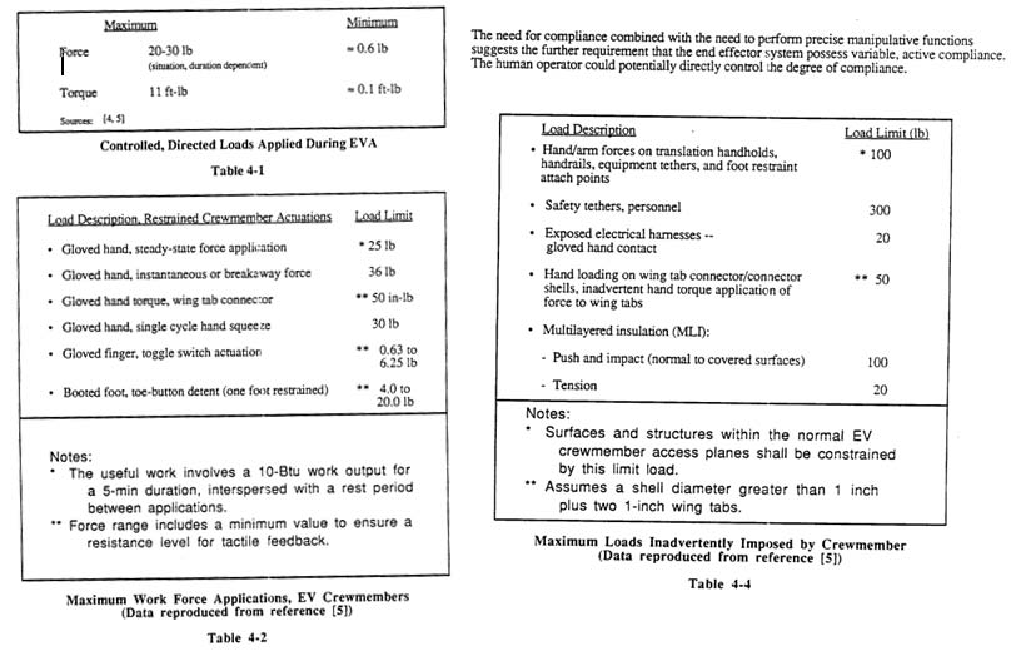
\includegraphics[scale=0.6]{Apppic/eeloads}
\caption[End Effector Load Limits]{End Effector Load Limits \cite{NASAEE_Mishkin}}
\end{figure}
\begin{figure}[H]
\centering
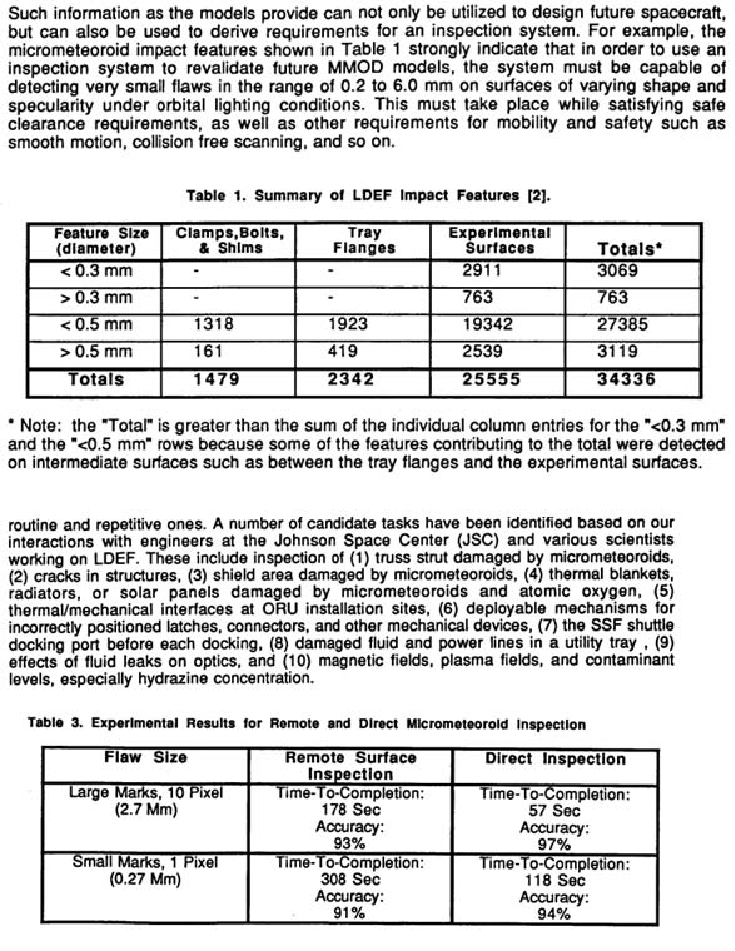
\includegraphics[scale=1]{Apppic/inspect}
\caption[Requirements for Inspection Systems]{Requirements for Inspection Systems \cite{NASAinspect_Hayati}}
\end{figure}
\newpage
\section{Power Consumption of various sensor types}
\label{app:sensorpower}
\begin{table}[H]
\centering
\caption{Power consumption of sensors}
\begin{tabular}{ccC{3cm}C{3cm}c}
\toprule
\textbf{Part}	&	\textbf{Count}	&	\textbf{Average Power (W)}	&	\textbf{Peak Power (W)}	&	\textbf{Voltage (V)}	\\\midrule
\textbf{Camera}	&	
3	&	1.75	&	2.5	&	5	\\
\textbf{Proximity Sensor}	&	
3	&	1.5	&	1.5	&	15	\\
\textbf{Force Sensor}	&	
2	&	1	&	1	&	5	\\
\textbf{Resolver}	&	
14	&	0.6	&	2	&	7	\\
\textbf{Torque Sensor}	&	
7	&	1	&	1	&	18	\\
\textbf{Lights}	&	
-	&	0	&	10	&	24	\\
\hline
\textbf{Total}	&	
-	&	27.15	&	59	&	-	\\\bottomrule
\end{tabular}
\label{tab:sensorpower}
\end{table}
\section{Joint Motion Range for Canadarm2 and ERA}
\label{app:jointrange}
\begin{table}[H]
\centering
\caption{Joint motion range for Canadarm2 and ERA}
\begin{tabular}{|c|c|c|}
\hline
	&	\textbf{Canadarm2 (Degree)}	&	\textbf{ERA(Degree)}	\\\hhline{|=|=|=|}
\textbf{Shoulder Roll}	&	$\pm$270	&	$\pm$270	\\
\textbf{Shoulder Yaw}	&	$\pm$270	&	$\pm$120	\\
\textbf{Shoulder Pitch}	&	$\pm$270	&	$\pm$120	\\
\textbf{Elbow Pitch}	&	$\pm$270	&	+30 to -176	\\
\textbf{Wrist Pitch}	&	$\pm$270	&	$\pm$120	\\
\textbf{Wrist Yaw}	&	$\pm$270	&	$\pm$120	\\
\textbf{Wrist Roll}	&	$\pm$270	&	$\pm$185	\\\hline
\end{tabular}
\label{tab:jointrange}
\end{table}

\end{document}
